% The original source files were:
% uiucthesis2009.dtx  (with options: `example')
\def\fileversion{v2.25a} \def\filedate{2009/10/10}
% Package and Class "uiucthesis2009" for use with LaTeX2e.
\documentclass[edeposit,fullpage]{latex/uiucthesis2009}

\usepackage{notoccite} % Avoid references in captions causing numbering issues due to TOC
\usepackage{amsmath} % Need for subequations
\usepackage{mathrsfs} %https://ctan.org/pkg/mathrsfs
\usepackage{amssymb} % amssymb-telda and math symbols
\usepackage{booktabs} % Allows fancy Tables
\usepackage{boxedminipage} % Boxes around figures
\usepackage{changepage} % Allows one to temporarily change right and left margins
\usepackage{cite} % Allows improved handling of numeric citations including automatic ordering and ranges of multiple cites
\usepackage{enumitem} % Allows one to easily change the labels for enumerate list
\usepackage[flushleft]{threeparttable} % This package allows for notes under tables.  Flushleft option flushes the note left margin of table (center is default)
% Load tabularx and xcolor before adjustbox to avoid conflict
\usepackage{tabularx} % Package which allows paragraphs in Tables
\usepackage[table]{xcolor} % Allows coloring of tables
\usepackage{graphicx} % Extends graphics package for figures. Provides optional arguments to the \includegraphics command
\graphicspath{{figures/}}
\usepackage[export]{adjustbox} % Extends the graphicx package to do trimming and other adjustments.
\usepackage{epstopdf} % Converts eps images to PDF to use in graphicx package.  Must be loaded after graphicx package
\usepackage[list=true,listformat=simple]{subcaption} % Allow for subfigures with captions in table of contents
\usepackage{bm}
\usepackage{commath}
\usepackage{multirow}

\usepackage{xspace} % Allows dynamic space in global text variables. This can allow you to just use \newCommandName rather than \newCommandName{}.
%%\usepackage[bookmarks=true,backref=page, hyperfigures=true, pdfpagelabels=false]{hyperref}
\usepackage[bookmarks=true,backref=page,hyperfigures=true,pdfpagelabels=false,hidelinks]{hyperref}

\usepackage{bookmark} % Eliminates Warning Bookmark level greater than one. Must be loaded after hyperref
\usepackage[capitalize]{cleveref}% https://ctan.org/pkg/cleveref % Must be loaded after hyperref
\creflabelformat{equation}{#2\textup{#1}#3}% Equation references don't have parentheses
\usepackage[utf8]{inputenc}
\usepackage[nogroupskip,toc,acronym]{glossaries} % place AFTER hyperref for hyperlinked glossary

\usepackage{lineno} % Provide line numbers for drafts

% User defined
% Add you own definitions here (file ANA-STDM-2018-27-INT1-defs.sty).
\usepackage{ANA-STDM-2018-27-INT1-defs}
\usepackage{siunitx} % A units package to format your units properly
\usepackage{atlasparticle}
\usepackage{atlasunit}
%%\usepackage{subfig} % Maybe removed later



% \linenumbers % uncomment if want draft printing

\begin{document}

\title{Thesis Title}
\author{Thesis Author}
\department{Physics}
\schools{Previous Degrees}
\phdthesis
\advisor{Ph.D Mark Neubauer}
\degreeyear{Current Year}
\committee{Committee Chair, Chair\\
           Theis Advisor, Director of Research\\
           Third Member of Committee\\
           Fourth Member of Committee}
\maketitle

\frontmatter

% Create an abstract that can also be used for the ProQuest abstract.
% Note that ProQuest truncates their abstracts at 350 words.
\begin{abstract}
The analysis searches for electroweak diboson ($WW/WZ/ZZ$) production in association with a high-mass dijet system, using data from proton-proton collisions at a center-of-mass energy of $\sqrt{s} = 13 TeV$. The analysis is performed in the semi-leptonic final states which include a hadronic decay boson and a leptonic decay one. The analysis is split into three channels according to the number of electrically charged leptons from the leptonic boson decay: 0-lepton channel, 1-lepton channel, and 2-lepton channel.
The focus of this thesis is an approach to enhance the separation between the VBS signal and the backgrounds in the 1-lepton channel using artificial neural network models. This approach is developed using Monte Carlo simulated events in the semi-leptonic VBS analysis and tested using ATLAS data for improving the sensitivity of the analysis to the target signal.
\end{abstract}

% Create a dedication in italics with no heading, centered vertically
% on the page.
\begin{dedication}
Write Dedication Here
\end{dedication}

% Create an Acknowledgements page, many departments require you to
% include funding support in this.
\chapter*{Acknowledgments}
This work was supported by the U.S. Department of Energy, Office of Science, High Energy Physics, under contract number DE-SC0023365.

Mark Neubauer, Viviana Cavelier, Matthew Feickert

Also, I would like to say thank you to my late grandparents. Though you might not have fully understood my work, I am grateful for every memory we shared. Finally, to my parents, Meizhen Zhu and Yuesong Zeng, who moved across continents to allow me to fulfill my dream of becoming a physicist: It has been a long journey, and I cannot thank you enough for your unwavering support and patience. There is still a long journey ahead of me, and I am determined to make you proud with every step I take.


% The thesis format requires the Table of Contents to come
% before any other major sections, all of these sections after
% the Table of Contents must be listed therein (i.e., use \chapter,
% not \chapter*).  Common sections to have between the Table of
% Contents and the main text are:
%
% List of Tables
% List of Figures
% List Symbols and/or Abbreviations
% etc.


\tableofcontents
\listoftables
\listoffigures
%% Create a List of Abbreviations. The left column
%% is 1 inch wide and left-justified
\chapter{List of Abbreviations}

%% List of Abbreviations, edit as needed
\begin{symbollist*}
\item[2HDM] Two-Higgs Doublet Model.
\item[AK4] An anti-$k_t$ jet with $R = 0.4$.
\item[ALICE] A Large Ion Collider Experiment.
\item[AM] Associated Memory.
\item[AMB] Associated Memory Board.
\item[ATCA] Advanced Telecommunications Computing Architecture.
\item[ATLAS] A Toroidal LHC ApparatuS.
\item[AUX] Auxiliary Board.
\item[AXW] AUX Wrapper.
\item[BR] Branching Ratio.
\item[CA12] A Cambridge/Aachen jet with $R = 1.2$.
\item[CC] Clock Correction.
\item[CERN] European Organization for Nuclear Research.
\item[CL] Confidence Level.
\item[CMS] Compact Muon Solenoid.
\item[CP] Combined Performance.
\item[CR] Control Region.
\item[DF] Data Formatter.
\item[DFW] DF Wrapper.
\item[DRAM] Dynamic Random Access Memory.
\item[DSP] Digital Signal Processing Block.
\item[ECAL] Electromagnetic Calorimeter.
\item[ECR] Event Count Reset.
\item[EGM] Extended Gauge Model.
\item[EF] Event Filter.
\item[ELID] Extended Level 1 Identifier.
\item[EXP] Extrapolator.
\item[EXTF] Extrapolator / Track Fitter.
\item[FC] Flow Control.
\item[FCAL] Forward Calorimeter.
\item[FE] Front End.
\item[FF] Flip Flop.
\item[FIFO] First In First Out.
\item[FLIC] FTK Level-2 Interface Crate.
\item[FPGA] Field Programmable Gate Array.
\item[FSR] Final State Radiation
\item[fSSB] Final Second Stage Board.
\item[FTK] Fast TracKer.
\item[GTX] Gigabit Transceiver.
\item[ggF] gluon Fusion.
\item[HEP] High Energy Physics.
\item[HLT] High Level Trigger.
\item[HP] High Purity.
\item[HVT] Heavy Vector Triplet.
\item[HW] Hit Warrior.
\item[HXMPP] Hit Memory++.
\item[IBL] Insertable B Layer.
\item[ID] Inner Detector.
\item[IM] Input Mezzanine.
\item[ISR] Initial State Radiation.
\item[JVF] Jet Vertex Fraction.
\item[JER] Jet Energy Resolution.
\item[JES] Jet Energy Scale.
\item[KK] Kaluza-Klein.
\item[L1] Level 1 Hardware Trigger.
\item[L2] Level 2 Hardware Trigger.
\item[LAMB] Local Associated Memory Board.
\item[LDC] Link Destination Card.
\item[LED] Light Emitting Diode.
\item[LFSR] Linear Feedback Shift Register.
\item[LHC] Large Hadron Collider.
\item[LHCb] Large Hadron Collider beauty.
\item[LINAC2] Linear Accelerator 2.
\item[LP] Low Purity.
\item[LSC] Link Source Card.
\item[LUT] Look Up Table.
\item[MC] Monte Carlo.
\item[MET] Missing Transverse Energy.
\item[MIG] Memory Interface.
\item[ML] Maximum Likelihood.
\item[MS] Muon Spectrometer.
\item[NLO] Next to Leading Order.
\item[NNLO] Next to Next to Leading Order.
\item[PDF] Parton Distribution Function.
\item[PIX] Pixel Detector.
\item[PU] Processing Units.
\item[PS] Proton Synchrotron.
\item[pSSB] Preliminary Second Stage Board.
\item[QCD] Quantum Chromo Dynamics.
\item[QSFP] Quad Small Form-factor Pluggable.
\item[RAM] Read Access Memory.
\item[RLDRAM] Reduced Latency DRAM.
\item[ROD] Read Out Driver.
\item[ROI] Region of Interest.
\item[ROM] Read Only Memory.
\item[ROS] Read Out System.
\item[RS] Randall-Sundrum.
\item[RTM] Rear Transmission Module.
\item[RX] Receiver.
\item[SCT] Semiconductor Tracker.
\item[SE] Sync Engine.
\item[SF] Scale Factor.
\item[SFP] Small Form-factor Pluggable.
\item[SLink] Super Link.
\item[SM] Standard Model.
\item[SPS] Super Proton Synchrotron.
\item[SR] Signal Region.
\item[SSB] Second Stage Board.
\item[SSID] Super Strip Identifier.
\item[TDAQ] Trigger and Data Acquisition.
\item[TF] Track Fitter.
\item[TFW] Track Fitter Wrapper.
\item[TileCAL] Hadronic Calorimeter.
\item[TRT] Transition Radiation Tracker.
\item[TX] Transmitter.
\item[VBF] Vector Boson Fusion.
\item[VME] VERSA-Module Euro.
\item[VR] Validation Region.
\end{symbollist*}

%% Symbol defs
\def\met{\ensuremath{E_{\mathrm{T}}^{\mathrm{miss}}}}

%% Create a List of Symbols. The left column
%% is 0.7 inch wide and centered
%% Edit as needed

\chapter{List of Symbols}

\begin{symbollist}[0.7in]
    \item[$\ell$] lepton.
    \item[$e$] electron.
    \item[$\mu$] muon.
    \item[$\tau$] tau.
    \item[$\nu_{e}$] electron neutrino.
    \item[$\nu_{\mu}$] muon neutrino.
    \item[$\nu_{\tau}$] tau neutrino.
    \item[$q$] quark, also used for charge.
    \item[$u$] up quark.
    \item[$d$] down quark.
    \item[$s$] strange quark.
    \item[$c$] charm quark.
    \item[$b$] bottom quark.
    \item[$t$] top quark.
    \item[$g$] gluon.
    \item[$\gamma$] photon.
    \item[$W$] $W$ boson.
    \item[$Z$] $Z$ boson.
    \item[$H$] Higgs boson.
    \item[$V$] Vector boson.
    \item[$p$] proton.
    \item[$n$] neutron.
    \item[$G^*$] RS graviton.
    \item[$G_{KK}$] KK graviton.
    \item[$W'$] Heavy $W$ boson.
    \item[$Z'$] Heavy $Z$ boson.
    \item[$V'$] Heavy Vector Boson.
    \item[$E_T^{miss}$] Missing transverse energy.
    \item[$E_T$] Transverse energy.
    \item[$p_T$] Transverse momentum.
    \item[$\eta$] pseudo rapidity.
    \item[$\theta$] polar angle.
    \item[$\phi$] azimuthal angle.
    \item[$d_0$] the distance to the $z$-axis at the perigee point.
    \item[$z_0$] the $z$-coordinate at the perigee point.
    \item[$\phi_0$] the azimuthal angle at the perigee point.
    \item[$\chi^2$] statistic that measures how good the data fits the track.
    \item[$R$] distance in $\eta-\phi$ space.
    \item[$j$] small-$R$ jet.
    \item[$J$] large-$R$ jet.
    \item[$g_f$] fermion coupling.
    \item[$g_H$] Higgs and vector boson coupling.
    \item[$g_\ell$] lepton coupling.
    \item[$g_q$] quark coupling.
    \item[$\sigma$] cross section.
    \item[$m$] mass.
    \item[fb] femto barn $= 10^{-43}~\mathrm{m}^2$.
    \item[eV] electron Volt $= 1.602 \times 10^{-19}~\mathrm{J}$.
\end{symbollist}


\mainmatter

\chapter*{Preface}\label{chapter:preface}
% c.f. https://tex.stackexchange.com/a/222961/152544
\addcontentsline{toc}{chapter}{\protect\numberline{}Preface}

The following is a summary of useful concepts in high energy particle physics.

\section{Units}\label{section:units}

Discussion of units

\section{Coordinates}\label{section:coordinates}

LHC coordinate systems

\section{Statistics}\label{section:statistics}

Statistics in particle physics


\chapter{Introduction}\label{chapter:introduction}

This is the first chapter of the dissertation.~\cite{PERF-2007-01}

\section{Creating Figures}\label{sec:figures}
\begin{figure}[htpb]
 \centering
 \includegraphics{introduction/example.pdf}
 \caption[Example placeholder figure with a citation~\cite{Higgs:1964ia} and shorter List of Figures caption.
  The List of Figures is protected from first use of glossary entries or acronyms like LHC.]{%
  This is a placeholder figure to act as an example.
  Here we cite a new reference in the caption to demonstrate that given the package configuration our order of references will not be distributed by the table of contents~\cite{Higgs:1964ia}.}\label{fig:test_figure}
\end{figure}

As can be seen in \Cref{fig:subfigure_example}, the subfigures are independent of each other such that \Cref{fig:subfigure_1} and \Cref{fig:subfigure_2} can be accessed separately.

\begin{figure}[htbp]
 \centering
 \begin{subfigure}[t]{0.48\textwidth}
  \centering
  \includegraphics[width=0.3\textwidth]{introduction/example.pdf}
  \caption[Short List of Figures captions work with subfigures too.]{%
   This is the first figure of two, in this example, and its own independent subfigure.}
  \label{fig:subfigure_1}
 \end{subfigure}%
 \quad
 \begin{subfigure}[t]{0.48\textwidth}
  \centering
  \includegraphics[width=0.3\textwidth]{introduction/example.pdf}
  \caption[Which makes the List of Figures readable and actually helpful.]{%
   As the \texttt{t} alignment option was chosen for the subfigures, they are still properly aligned vertically even though this caption is longer.}
  \label{fig:subfigure_2}
 \end{subfigure}
 \caption{An example of a figure that consists of two subfigures.}
 \label{fig:subfigure_example}
\end{figure}

As an example of an equation formatted in ``\href{https://www.overleaf.com/learn/latex/Display_style_in_math_mode}{display style}'' the equation for the fiducial cross section from~\cite{STDM-2015-05} is reproduced as \Cref{eq:fiducial_cross_section}:
\begin{equation}
 \sigma_{\mathrm{inel}}^{\mathrm{fid}} \left(\zeta > 10^{-6}\right) = \frac{N - N_{\mathrm{BG}}}{\epsilon_{\mathrm{trig}} \times \mathcal{L}} \times \frac{1 - f_{\zeta < 10^{-6}}}{\epsilon_{\mathrm{sel}}}
 \label{eq:fiducial_cross_section}
\end{equation}

\section{Creating Tables}\label{sec:tables}

To create tables in \LaTeX{} it is highly recommended to use the \href{https://www.ctan.org/pkg/booktabs}{\texttt{booktabs}} package.
It allows for very elegant and clean table creation, such as \Cref{table:natural_units}.
If you want to create a table quickly, or have a CSV file that you'd like to quickly turn into a table there are various \href{https://www.tablesgenerator.com/}{online \LaTeX{} table generators}.

\begin{table}[htpb]
 \centering
 \caption[Common quantities in particle physics in natural and SI units.]{%
  Common quantities in particle physics given in both natural units and SI units.}
 \begin{tabular}{@{}llll@{}} \toprule
  Quantity         & Natural Units                 & Natural Units (dimensionful)            & SI Units                                              \\ \midrule
  Speed            & $1$                           & $c$                                     & $3.0\times 10^{8}~\mathrm{m}/\mathrm{s}$              \\
  Angular Momentum & $1$                           & $\hbar$                                 & $10^{34}~\mathrm{m}^2 \,\mathrm{kg}/\mathrm{s}$       \\
  Energy           & $\mathrm{GeV}$                & $\mathrm{GeV}$                          & $1.6\times 10^{-10}~\mathrm{J}$                       \\
  Momentum         & $\mathrm{GeV}$                & $\mathrm{GeV}/c$                        & $1\times 10^{-19}~\mathrm{kg}\,\mathrm{m}/\mathrm{s}$ \\
  Mass             & $\mathrm{GeV}$                & $\mathrm{GeV}/c^{2}$                    & $1.8\times 10^{-27}~\mathrm{kg}$                      \\
  Time             & $1/\mathrm{GeV}$              & $\hbar/\mathrm{GeV}$                    & $6.6\time 10^{-25}~\mathrm{s}$                        \\
  Length           & $1/\mathrm{GeV}$              & $\hbar c/\mathrm{GeV}$                  & $2\times 10^{-16}~\mathrm{m}$                         \\
  Electric Charge  & $1$                           & $e/\sqrt{4\pi \alpha_{\mathrm{em}}}$    & $5.3\times 10^{-19}~\mathrm{C}$                       \\
  Magnetic Field   & $\left(\mathrm{GeV}\right)^2$ & $\left(\mathrm{GeV}\right)^2/\hbar c^2$ & $5\times 10^{16}~\mathrm{T}$                          \\
  \bottomrule
 \end{tabular}\label{table:natural_units}%
\end{table}

Good table design requires some thought and work, so it may be worth a look through some examples:
\begin{itemize}
 \item \href{https://tex.stackexchange.com/questions/238503/tip-on-how-to-make-a-visually-good-table}{TeX StackExchange: Tip on how to make a visually good table}
 \item \href{https://twitter.com/edwardtufte/status/451820483109847040?lang=en}{Edward Tufte endorsed} example from \href{http://static1.squarespace.com/static/56713bf4dc5cb41142f28d1f/t/56fd4c83746fb9261146eed5/1459440776291/ClearOffTheTableMd.gif}{Darkhorse Analytics}
\end{itemize}

\section{Dealing with Widows and Orphans}\label{sec:widos_and_orphans}

To reduce the difficulty of dealing with widowed text (the last line of a paragraph at the start of a page) and orphaned text (the first line of paragraph at the end of a page) the \href{https://ctan.org/pkg/nowidow?lang=en}{\texttt{nowidow}} package is used.
However, that doesn't solve the issue of orphaned section titles.
The user must manually do this, but the following \href{https://texfaq.org/FAQ-widows}{simple advice from \TeX{} FAQ} is recommended:

\begin{quote}
 Once you've exhausted the automatic measures, and have a final draft you want to ``polish'', you should proceed to manual measures.
 To get rid of an orphan is simple: precede the paragraph with \texttt{\textbackslash clearpage} and the paragraph can’t start in the wrong place.
\end{quote}


%1-lep DNN ML
%Motivations and Architecture
\section{Motivations and Architecture}
\label{sec:motivations_and_architecture}

Within the analysis framework, I have adopted a machine learning strategy, termed the Deep Neural Network (DNN) approach, to improve sensitivity to the VBS signal. This method utilizes neural network models implemented using Keras~\cite{chollet2015keras}, with TensorFlow serving as the backend~\cite{tensorflow2015-whitepaper}. Figure~\ref{fig:DNNArchitecturePic} illustrates the architecture of the DNN, which features multiple dense layers. The configuration of these layers, including the number of nodes and the specific setup, is detailed in Table~\ref{tab:1lepDNN layers}.
The hidden layers of the DNN employ the ReLU (rectified linear unit) function for activation. Alongside, L2 regularization is incorporated to minimize the risk of overfitting by penalizing the magnitude of the coefficients, thus maintaining model simplicity and robustness. The output layer utilizes a sigmoid activation function, ideal for binary classification tasks as it maps predictions to a probability scale, generating DNN scores that span a continuous range from zero to one.

\begin{figure}[ht]
       \centering
       \subfloat[]{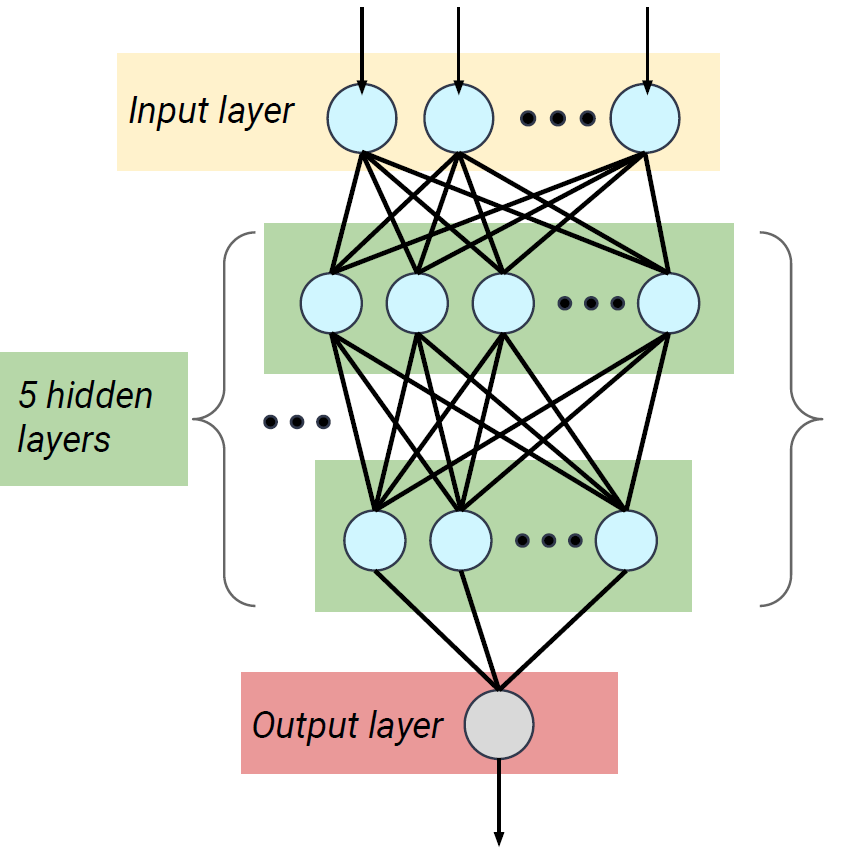
\includegraphics[width=0.55\textwidth]{figures/ml_dnn/DNNArchitecture.png}}
       \caption{Simplified DNN architecture visualisation.}
       \label{fig:DNNArchitecturePic}
\end{figure}

\begin{table}[ht]
    \centering
    \begin{tabular}{c|c|c|c}
     Layer(type) & Number of Neurons & Activation Functions & Regularizers\\
     \hline
     \hline
     Layer1(dense) & 64 & ReLu & L2\\
     Layer2(dense) & 32 & ReLu & L2\\
     Layer3(dense) & 32 & ReLu & L2\\
     Layer4(dense) & 32 & ReLu & L2\\
     Layer5(dense) & 16 & ReLu & L2\\
     Layer Out(dense) & 1 & Sigmoid & -\\
    \end{tabular}
    \caption{1-lepton DNN structure in merged and resolved signal regions.}
    \label{tab:1lepDNN layers}
\end{table}

\section{Input Variables and Feature Engineering}
\label{input_variables}

We assess the impact of input features on our DNNs using SHAP (SHapley Additive exPlanations), as introduced by Lundberg and Lee~\cite{LundbergLee2017}. SHAP quantifies the contribution of each feature to the deviation of a particular prediction from the average outcome across the dataset. This method provides a game theory-based interpretable approximation of complex neural networks, facilitating a deeper understanding of how individual features influence the model's predictions (DNN scores) for specific events. Employing SHAP values helps create a simplified yet faithful model that mirrors the original network's performance, making the decision-making process transparent and easier to interpret.

To optimize the DNN models, we use a backward feature elimination method, guided by SHAP value rankings, which is a recognized technique in feature selection. This approach involves systematically removing the least important input features, as determined by SHAP values, and then retraining the DNN models after each round to assess the impact of these eliminations on model performance. SHAP values are recalculated after each training session to ensure that the feature rankings are continuously updated. In the end, we retain 15 input features for the merged category and 17 for the resolved category, demonstrating tailored optimizations for each.
The final selection of input features for both categories is documented in Table~\ref{tab:1lepNN}, and their corresponding SHAP value rankings are illustrated in Figure~\ref{fig:1lepDNN_shap_rank}.

The term ``full system'' refers to variables associated with the entire set of signal jet(s), lepton(s), and tagging jets.
The boson centrality, $\xi(V)$, is defined as :  
\begin{equation} \label{eq:centr} \xi(V)  = min(\Delta\eta_{-},\Delta\eta_{+}) \end{equation} where $$\Delta\eta_{-} = min(\eta_{\Vlep},\eta_{\Vhad}) - min(\etajo,\etajt)$$ and  $$\Delta\eta_{+} = max(\etajo,\etajt) - max(\eta_{\Vlep},\eta_{\Vhad}) $$
Figures~\ref{fig:mer_inputs-part1}, \ref{fig:mer_inputs-part2}, \ref{fig:res_inputs-part1}, and \ref{fig:res_inputs-part2} display the distributions of input features within the SRs. The noticeable differences in distribution shapes between the signal and background MC samples, as shown in these figures, highlight the effectiveness of our feature selection process.

Figure~\ref{fig:ROCChecks} presents a comparison of the performance metrics for the initial and final DNN models in both the merged and resolved categories, demonstrating that both models achieve comparable levels of effectiveness. To better understand this comparison, 
we define signal efficiency and background rejection as follows:

\begin{equation}
\text{Signal Efficiency} = \frac{\text{Number of Signal events with DNN} > X}{\text{Total Number of Signal events}}
\end{equation}

\begin{equation}
\text{Background Rejection} = \frac{\text{Number of Background events with DNN} < X}{\text{Total Number of Background events}}.
\end{equation}

\begin{figure}[ht]
      \centering
       \subfloat[\emph{ROC Curve}]{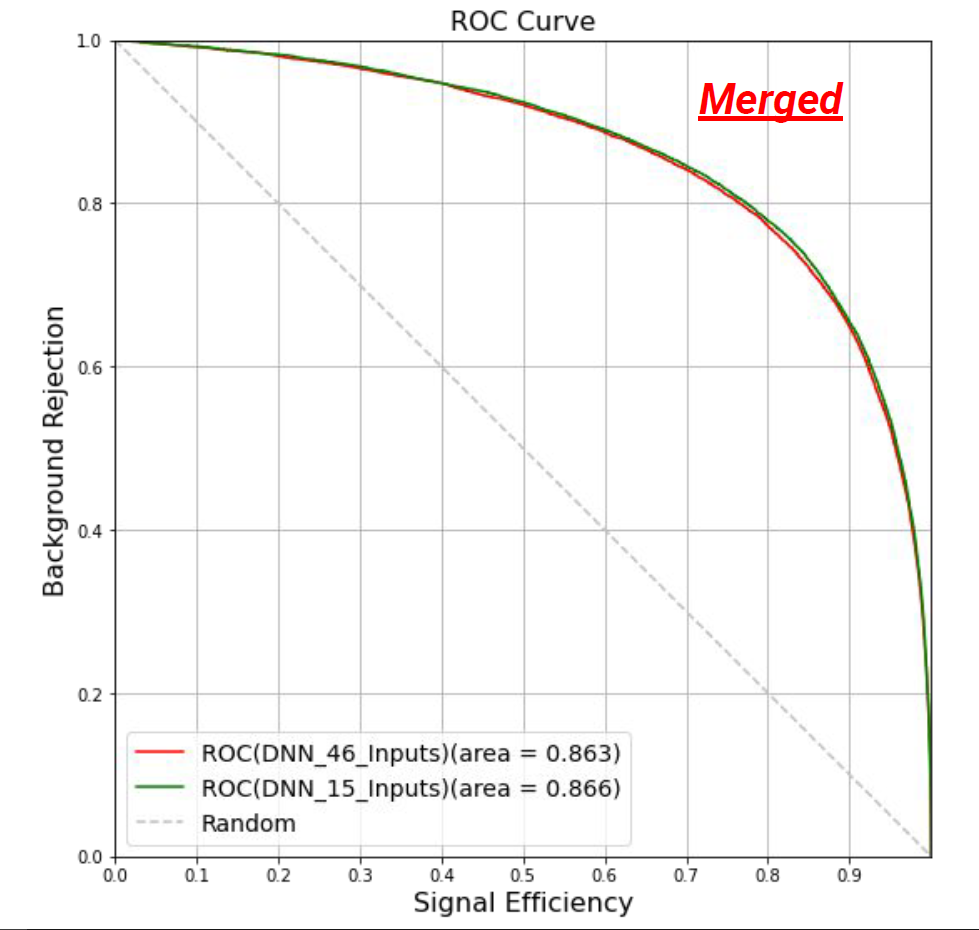
\includegraphics[width=0.4\textwidth]{figures/ml_dnn/ROCImpactMerged.png}}
       \subfloat[\emph{ROC Curve}]{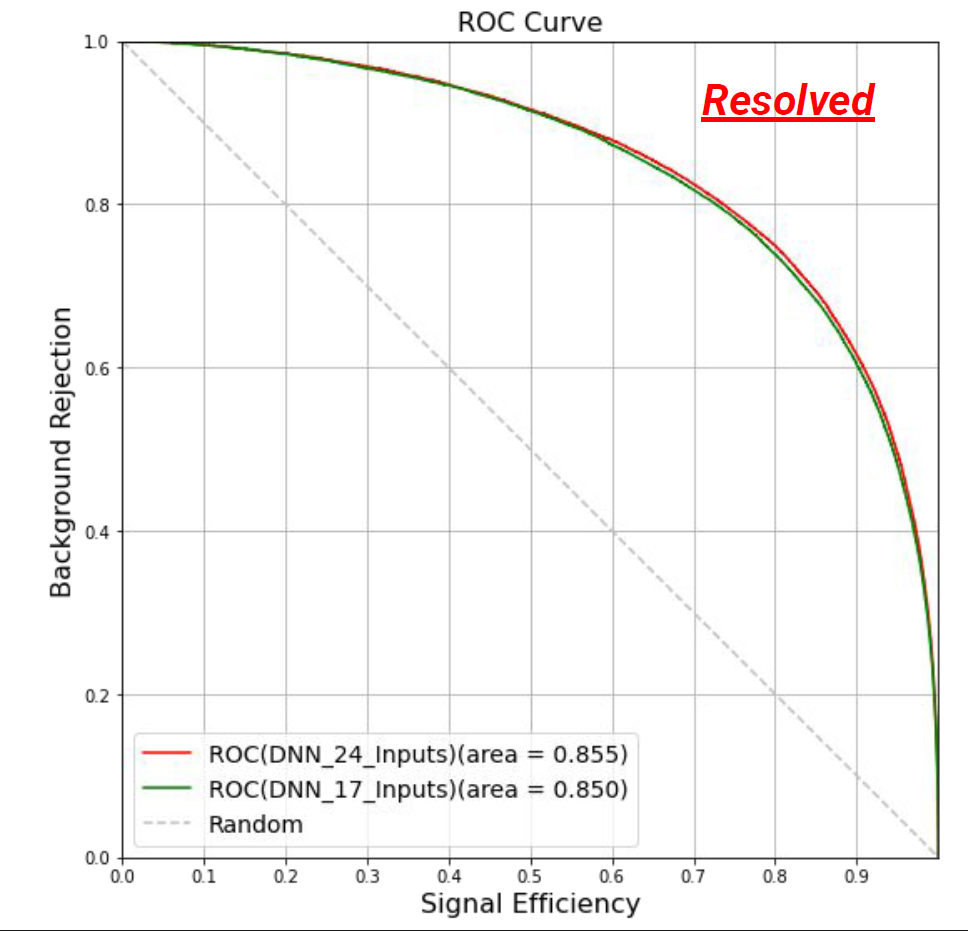
\includegraphics[width=0.4\textwidth]{figures/ml_dnn/ROCImpactRes.png}}
       \caption{ROC curves for the DNN models in the merged (a) and resolved (b) categories. Here, ``area'' refers to the AUC (Area Under the ROC Curve). The AUC values are computed to offer quantitative measures of performance.}
       \label{fig:ROCChecks}
\end{figure}

\begin{table}[ht]
    \centering
    \begin{tabular}{r|c|c}
     feature & merged & resolved\\
     \hline
     \hline
     signal jet(s) mass & $m(J^\text{sig})$ & $m(jj^\text{sig})$\\
     signal jet transverse momentum & $ - $ & $p_\text{T}(j^\text{sig}_\text{lead})$ and  $p_\text{T}(j^\text{sig}_\text{sublead})$\\
     signal jet width & $ - $ & $W(j^\text{sig}_\text{lead})$ and  $W(j^\text{sig}_\text{sublead})$\\
     dijet(signal jet) transverse momentum & $ - $ & $p_\text{T}(jj^\text{sig})$\\
     number of tracks associated to the signal jet(s) & $N_\text{trk}(J^\text{sig})$ & -\\
     multiplicity of B-tagged jets & $N(j^\text{B-tagged})$ & -\\
     multiplicity of forward jets & $N(j^\text{forward})$ & -\\
     multiplicity of track jets & - & $N(j^\text{track})$\\
     diboson mass & $m(V^\text{had}V^\text{lep})$ & $ - $\\
     leading tagging jet mass & $m(j^\text{tag}_\text{lead})$ & $ - $\\
     full system mass & $ - $ & $m(V^\text{had}V^\text{lep}+jj^\text{tag})$\\
     tagging jet transverse momentum & $p_\text{T}(j^\text{tag}_\text{sublead})$ & $p_\text{T}(j^\text{tag}_\text{lead})$ and $p_\text{T}(j^\text{tag}_\text{sublead})$\\
     tagging jet width & $W(j^\text{tag}_\text{lead})$ and $W(j^\text{tag}_\text{sublead})$  & $ - $\\
     boson centrality & $\xi(V)$ & $ - $\\
     pseudo-rapidity of tagging jets & - & $\eta(j^\text{tag}_\text{lead})$ and $ \eta(j^\text{tag}_\text{sublead})$\\
     pseudo-rapidity of lepton & - & $\eta(l)$\\
     lepton transverse momentum & $p_\text{T}(l)$ & -\\
%%%     jets multiplicity & \multicolumn{2}{c}{$N(j)$}\\
     number of tracks associated to the tagging jets & $N_\text{trk}(j^\text{tag}_\text{lead})$ and $N_\text{trk}(j^\text{tag}_\text{sublead})$ & -\\
     jets multiplicity & \multicolumn{2}{c}{$N(j)$}\\
     tagging jets mass & \multicolumn{2}{c}{$m(jj^\text{tag})$}\\
     tagging jet separation & \multicolumn{2}{c}{$\Delta\eta(j^\text{tag}_\text{lead},j^\text{tag}_\text{sublead})$}\\
     lepton energy & \multicolumn{2}{c}{$E_{\ell}$}\\
    \end{tabular}
    \caption{Input variables for the 1-lepton DNN in merged and resolved signal regions.}
    \label{tab:1lepNN}
\end{table}

\begin{figure}[ht]
      \centering
       \subfloat[\emph{Rankings Merged}]{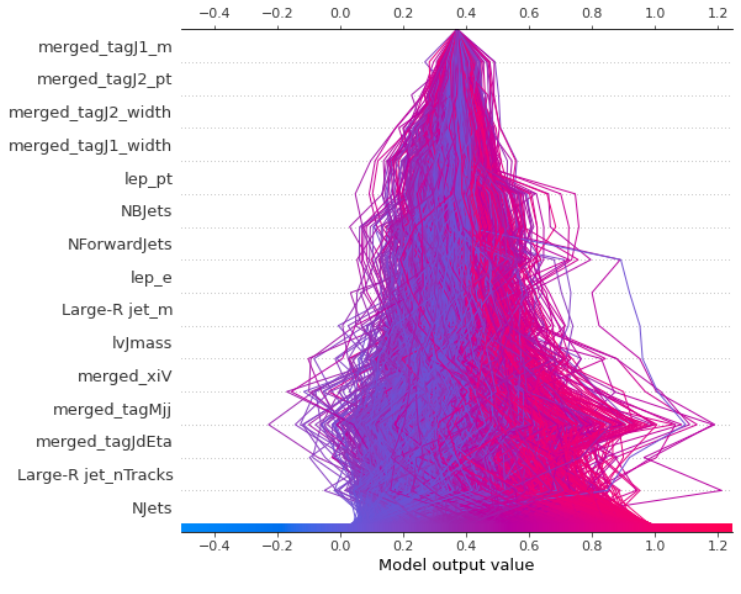
\includegraphics[width=0.4\textwidth]{figures/ml_dnn/rankings/decision_plot_mer.PNG}}
       \hspace{5mm}
       \subfloat[\emph{Rankings Resolved}]{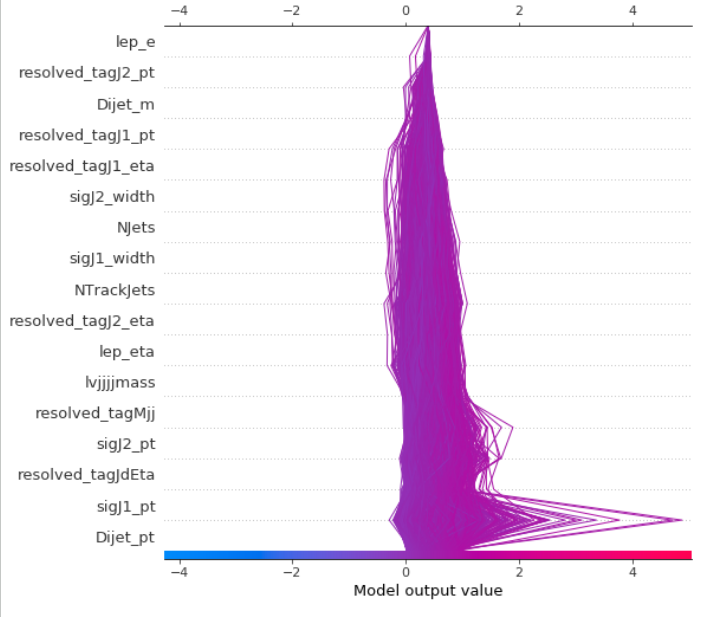
\includegraphics[width=0.4\textwidth]{figures/ml_dnn/rankings/decision_plot_res.PNG}}
       \caption{SHAP value rankings of input variables for both merged and resolved regimes; variables with lower impact appear at the top.}
       \label{fig:1lepDNN_shap_rank}
\end{figure}

\begin{figure}[ht]
 \centering
  % Row 1
  \subfloat[]{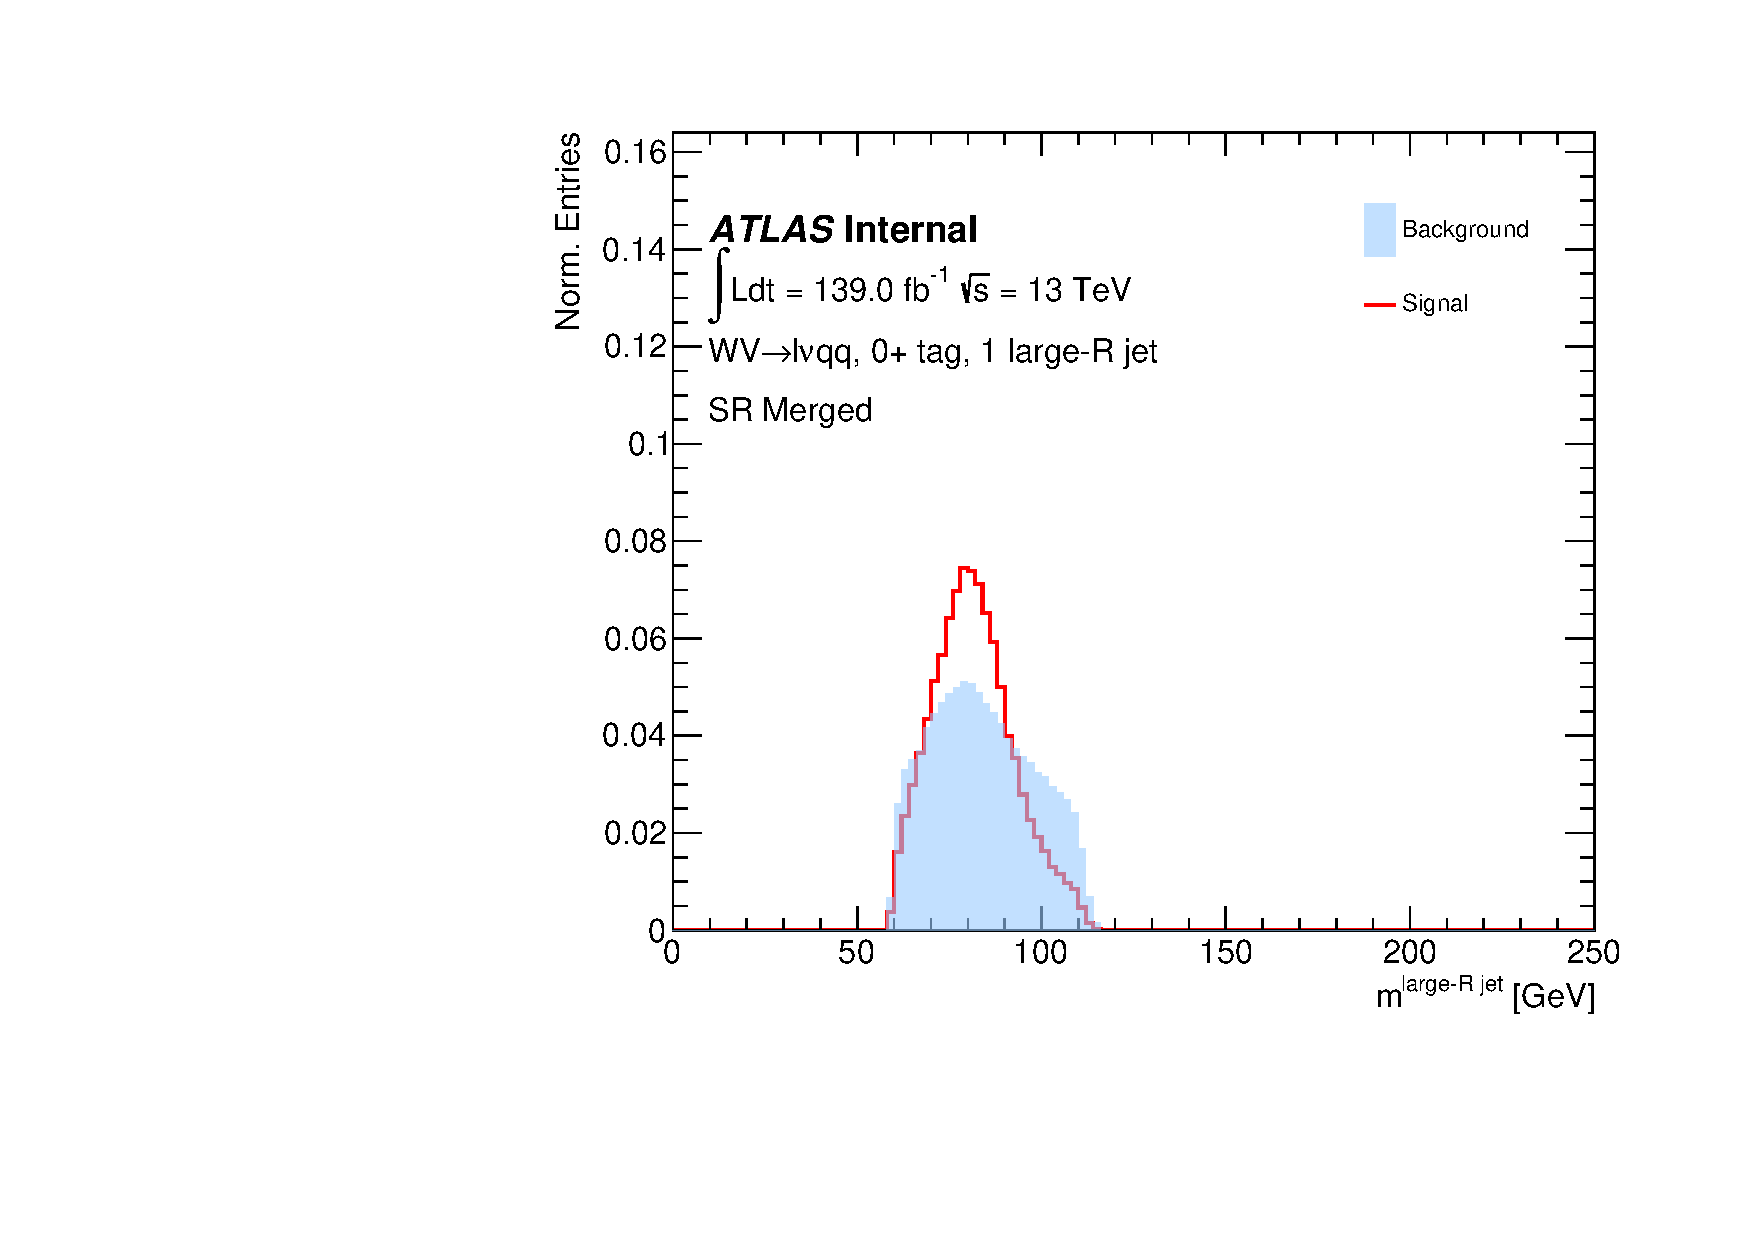
\includegraphics[width=0.3\textwidth]{figures/ml_dnn/variables/SR_Mer/norm_plot_fatJ_m.pdf}}\quad
  \subfloat[]{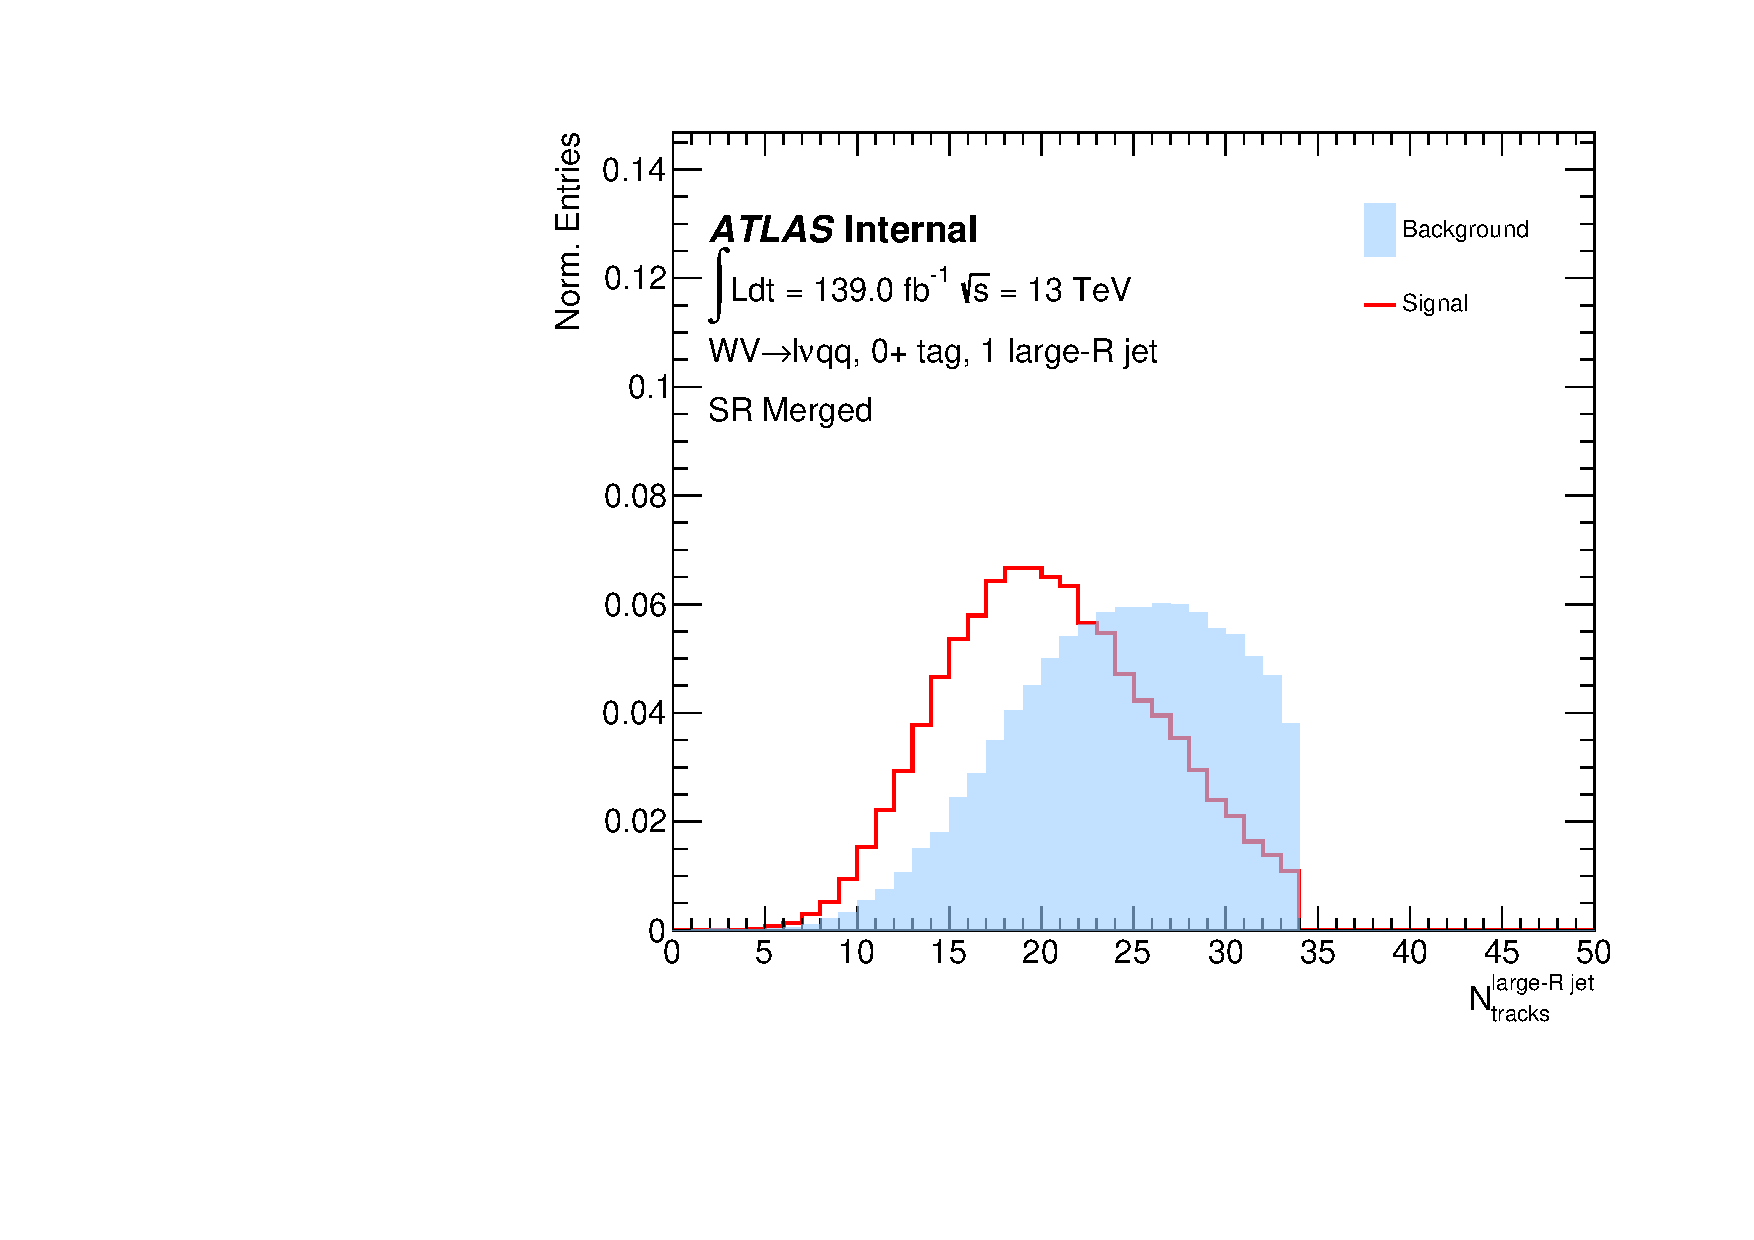
\includegraphics[width=0.3\textwidth]{figures/ml_dnn/variables/SR_Mer/norm_plot_fatJ_nTracks.pdf}}\quad
  \subfloat[]{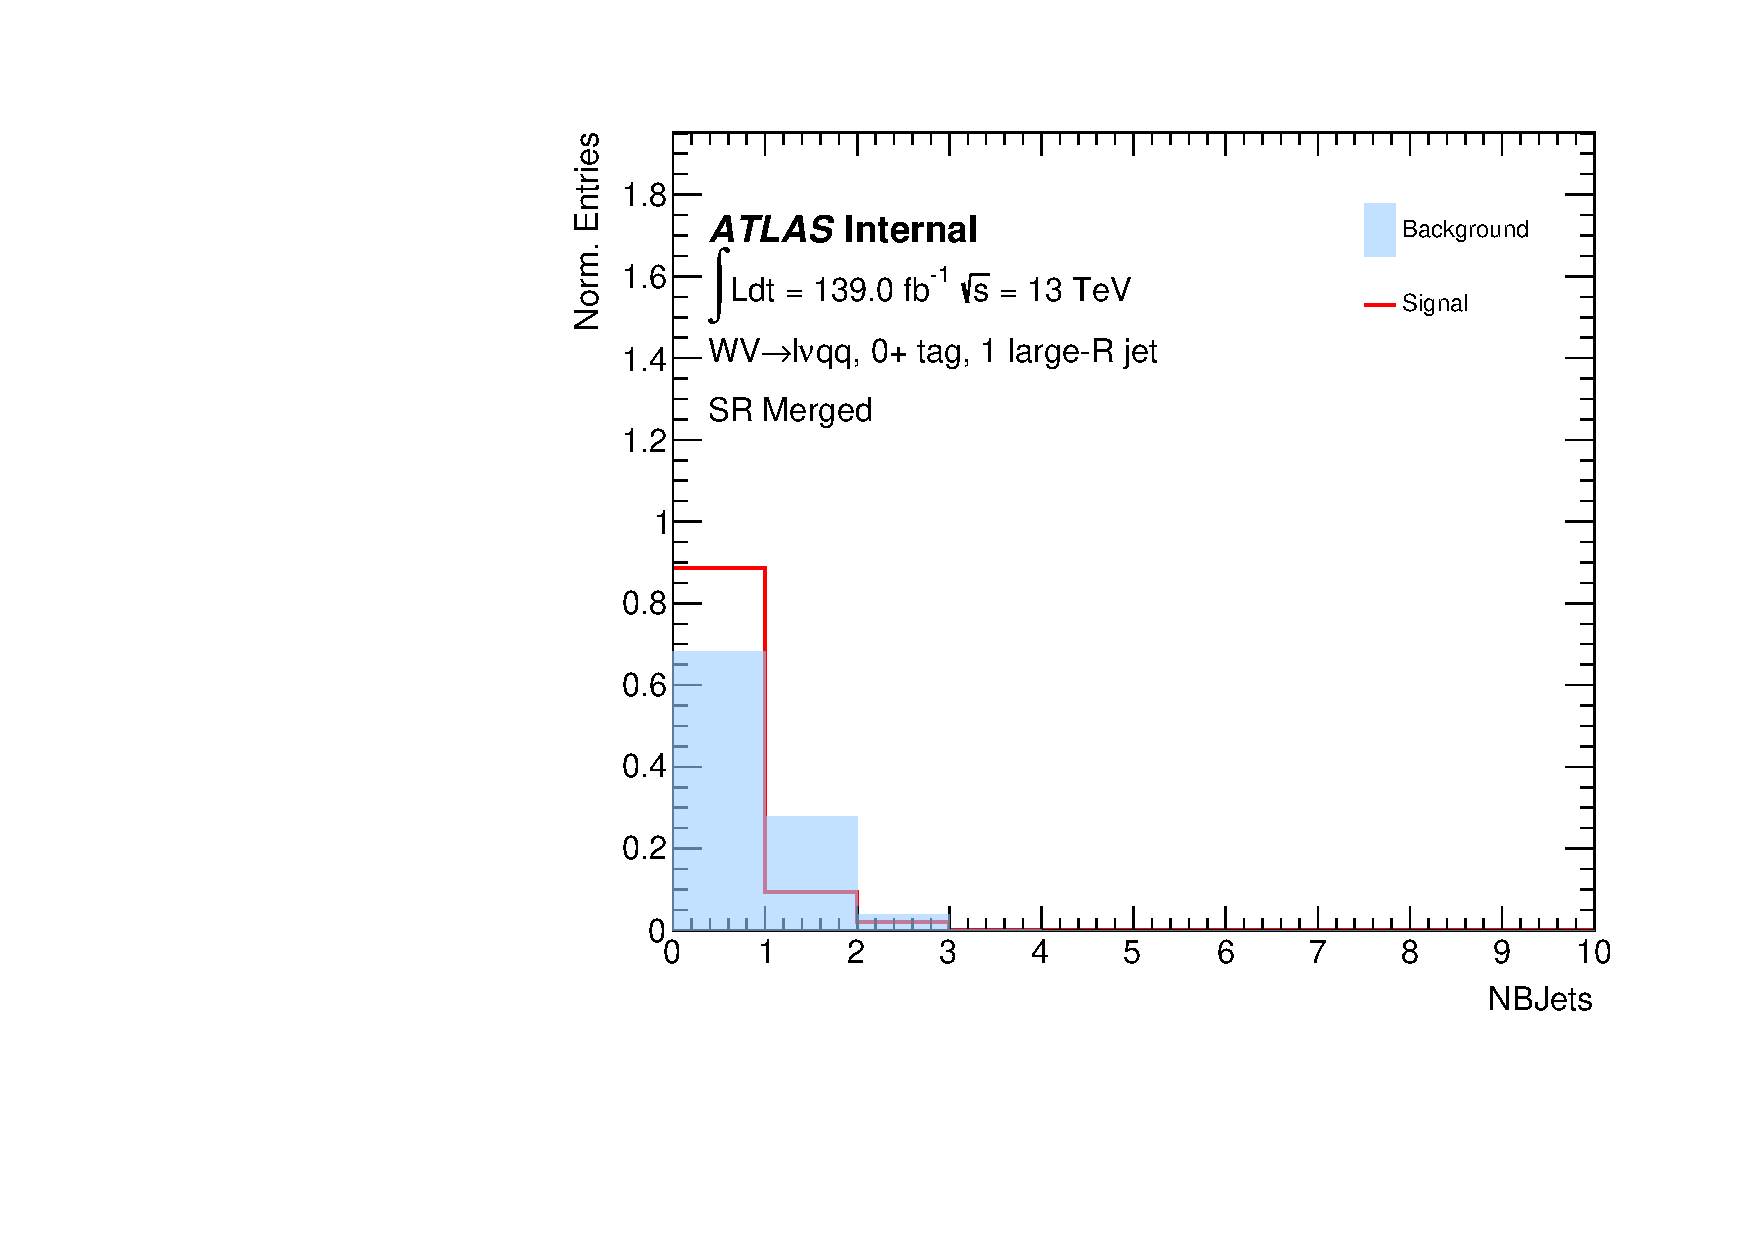
\includegraphics[width=0.3\textwidth]{figures/ml_dnn/variables/SR_Mer/norm_plot_NBJets.pdf}}

  % Row 2
  \subfloat[]{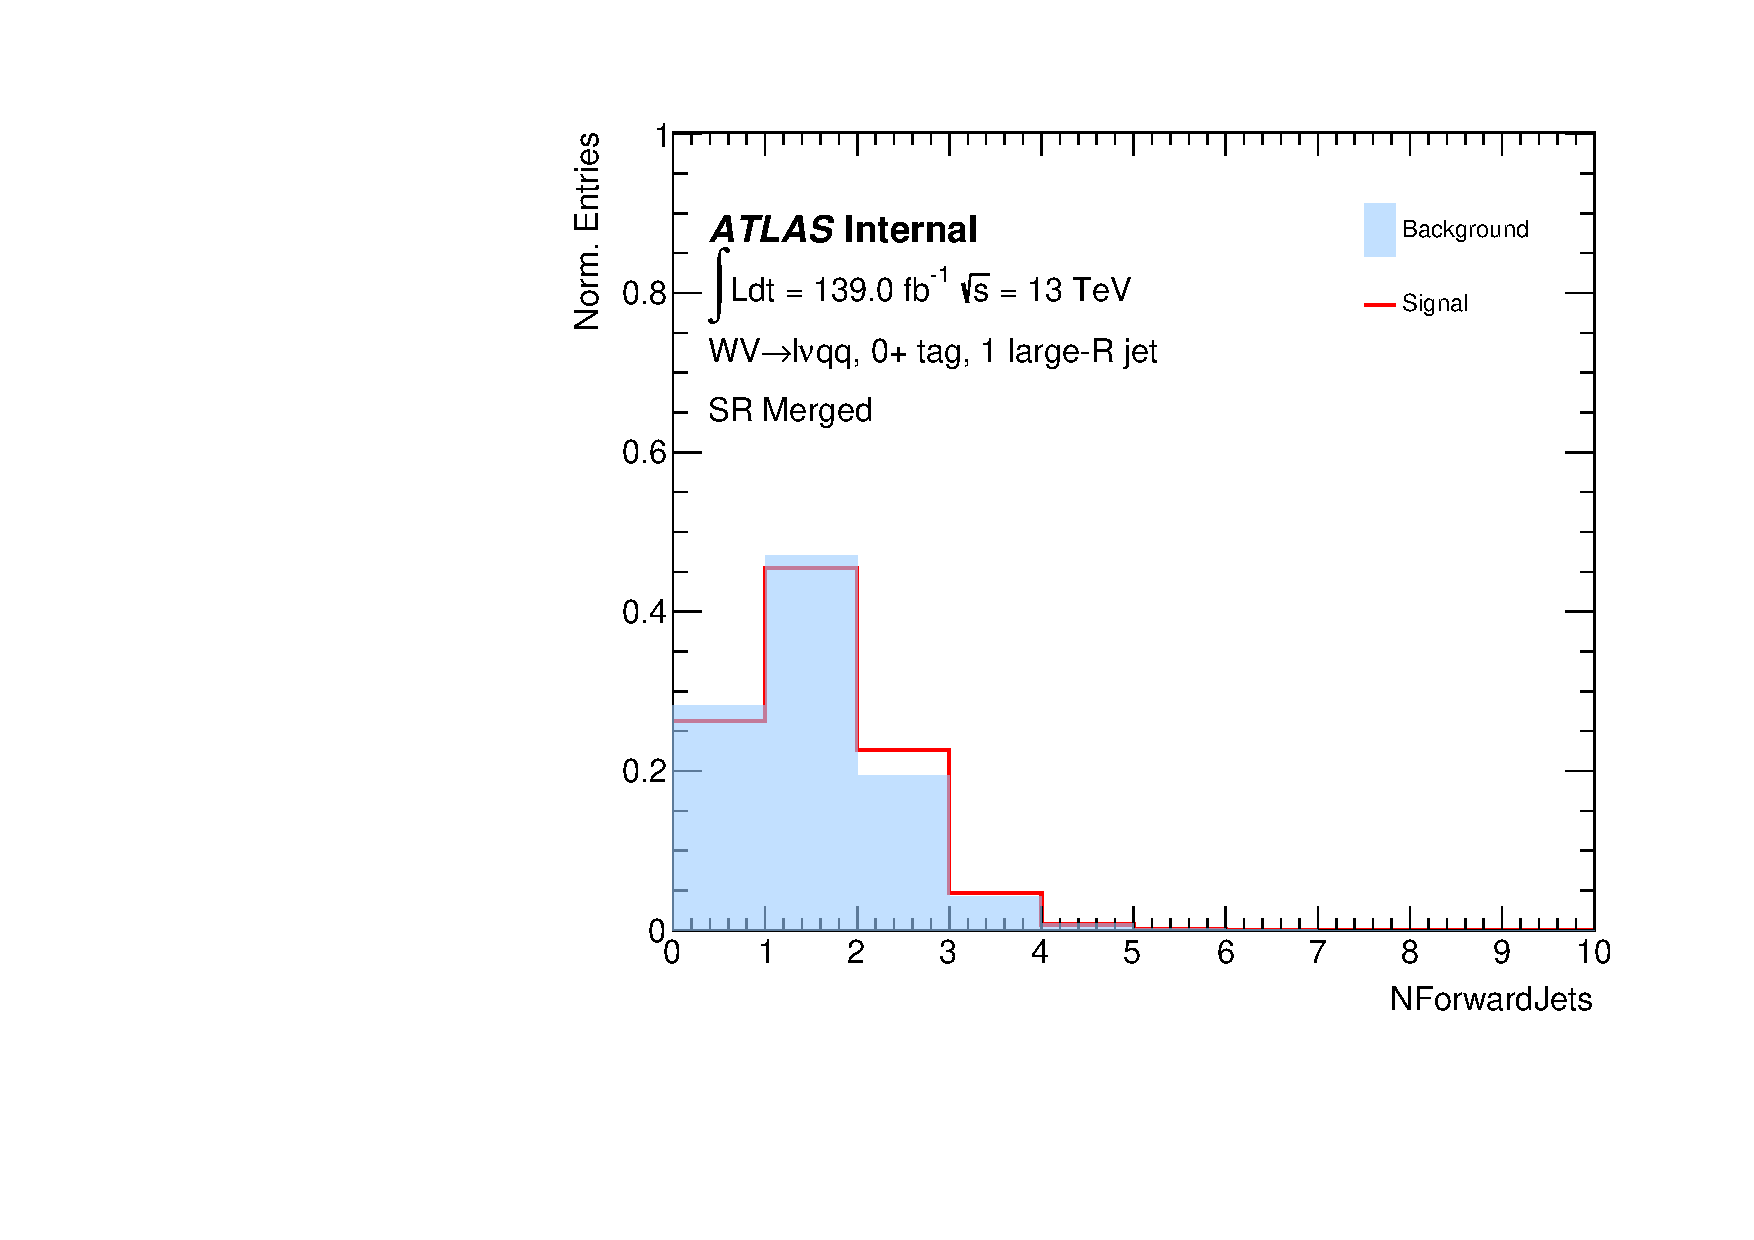
\includegraphics[width=0.3\textwidth]{figures/ml_dnn/variables/SR_Mer/norm_plot_NForwardJets.pdf}}\quad
  \subfloat[]{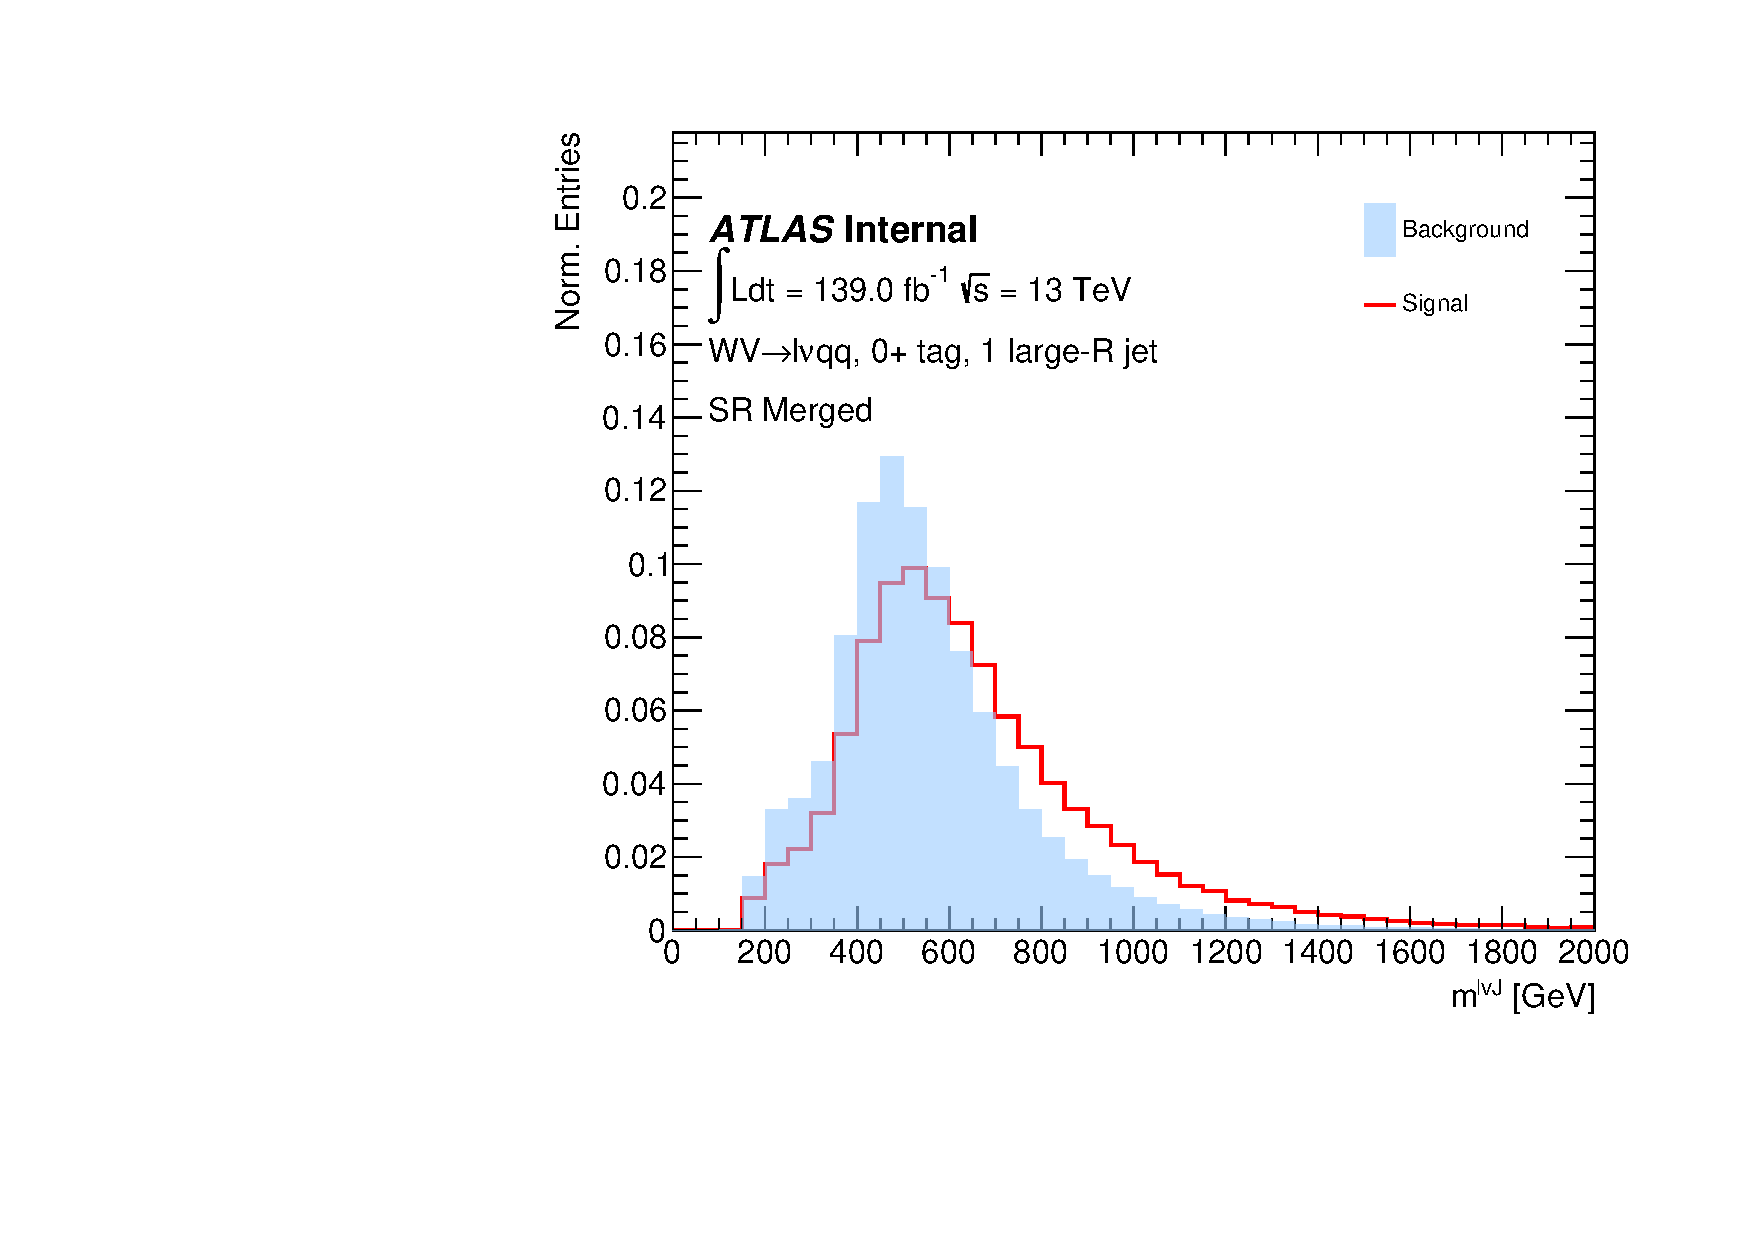
\includegraphics[width=0.3\textwidth]{figures/ml_dnn/variables/SR_Mer/norm_plot_lvJmass.pdf}}\quad
  \subfloat[]{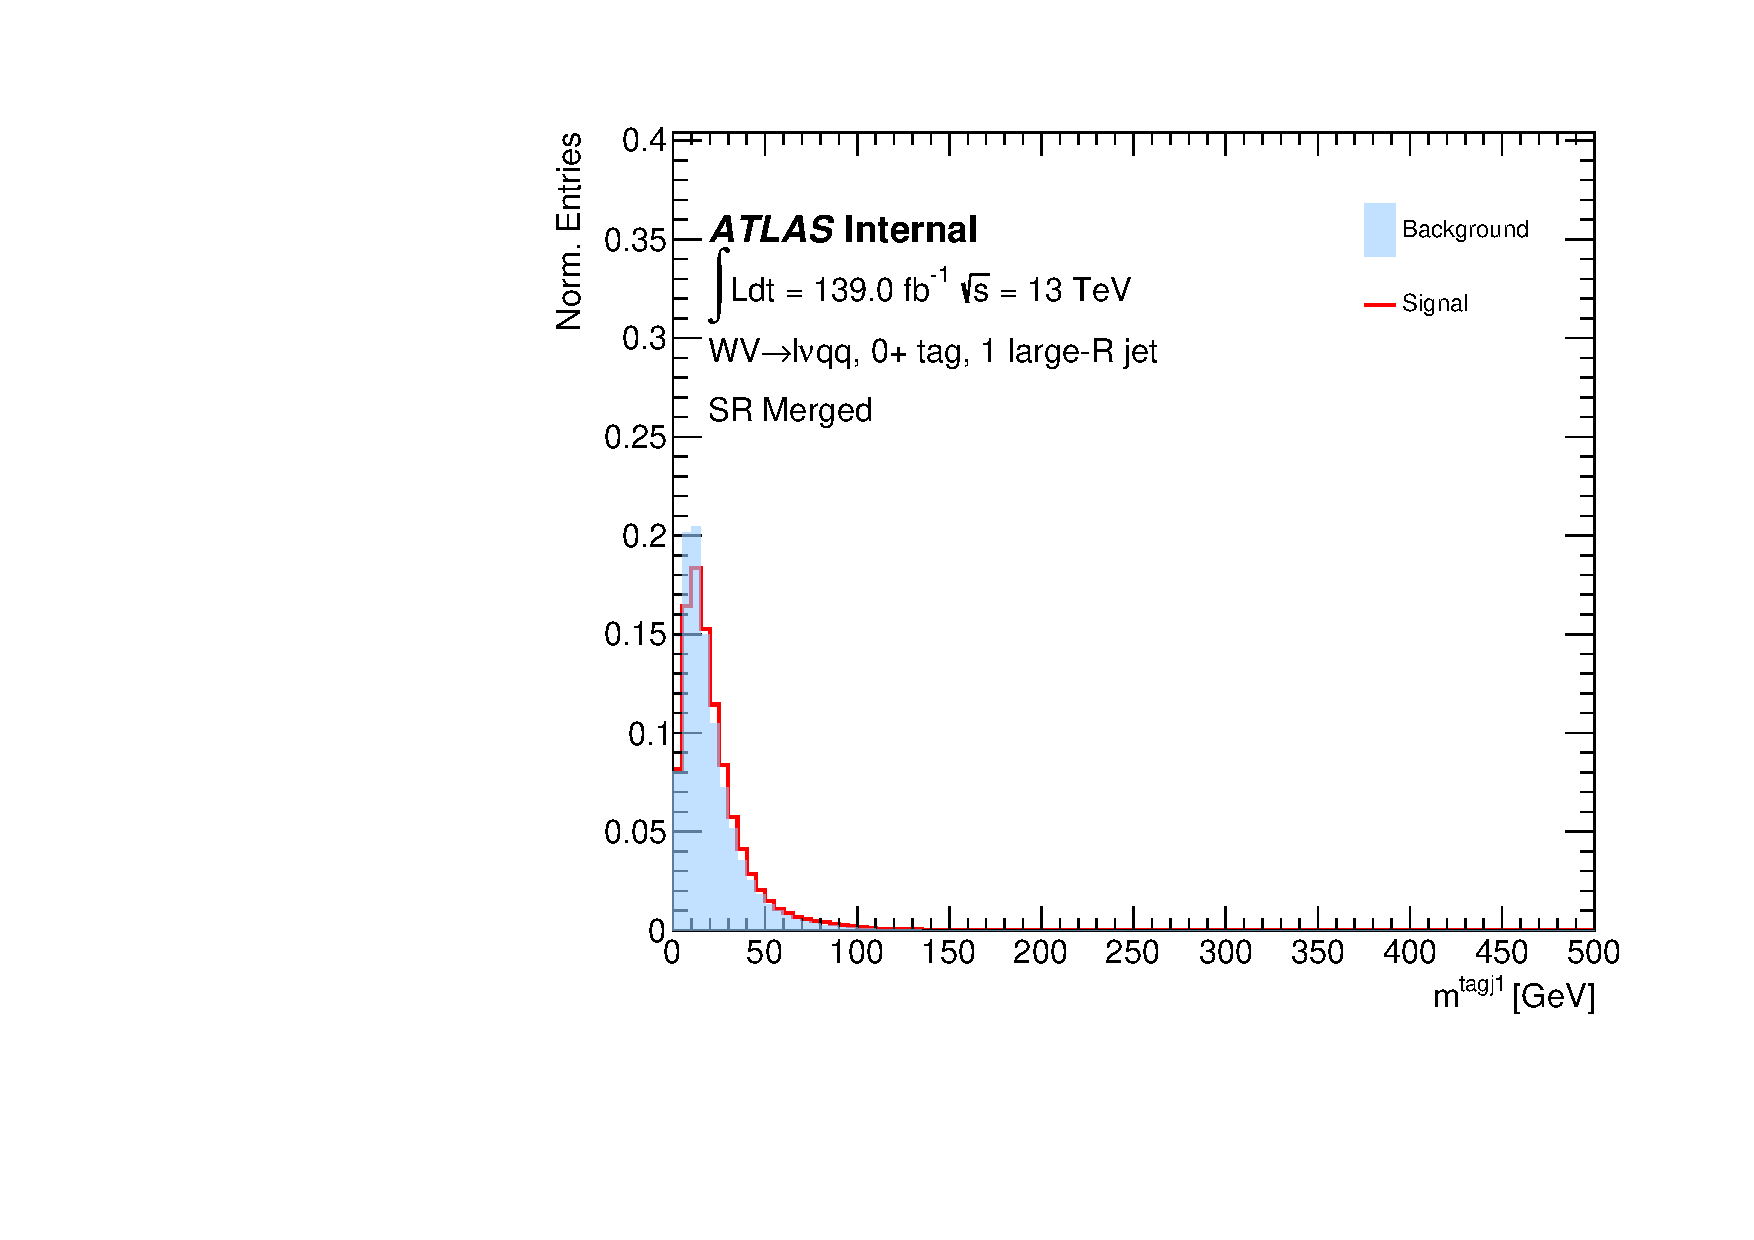
\includegraphics[width=0.3\textwidth]{figures/ml_dnn/variables/SR_Mer/norm_plot_merged_tagJ1_m.pdf}}

  % Row 3
%%  \subfloat[]{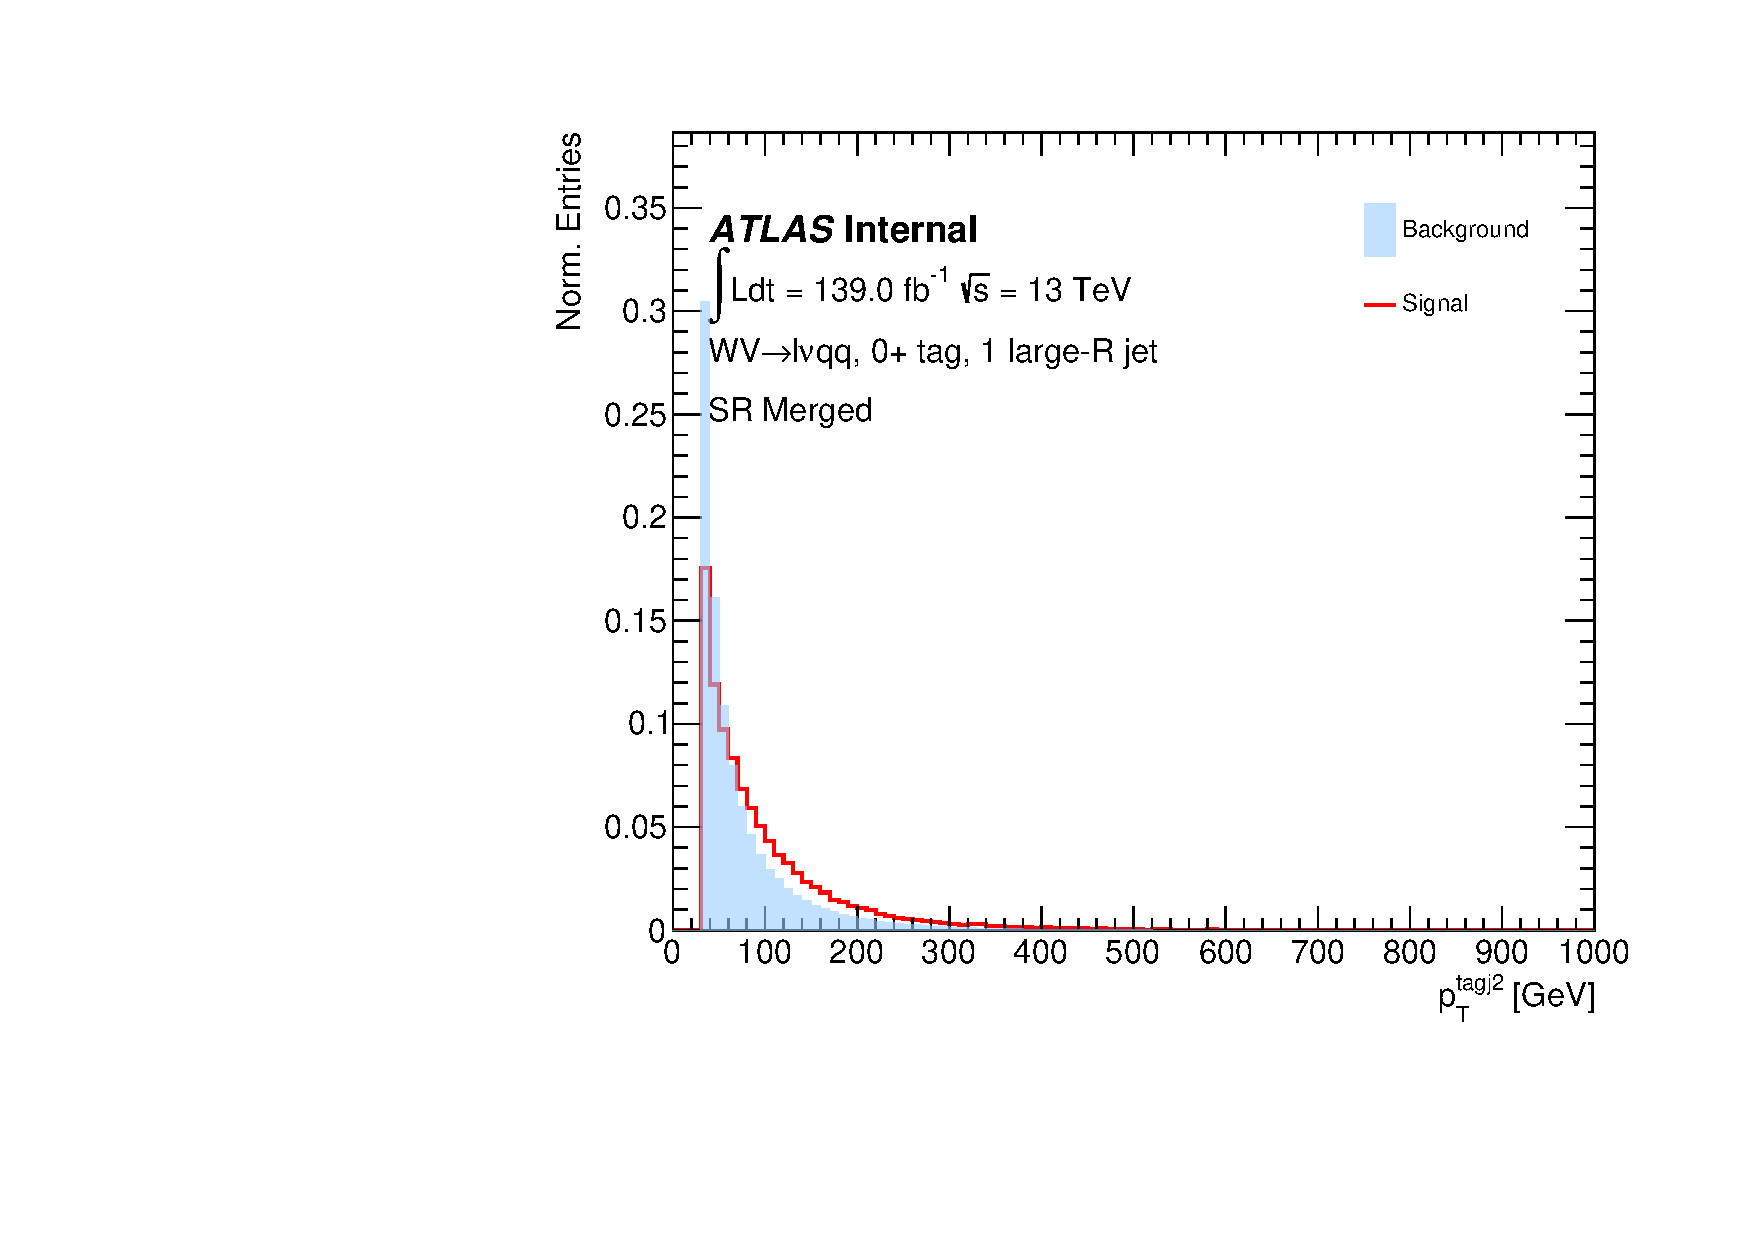
\includegraphics[width=0.3\textwidth]{figures/ml_dnn/variables/SR_Mer/norm_plot_merged_tagJ2_pt.pdf}}\quad
%%  \subfloat[]{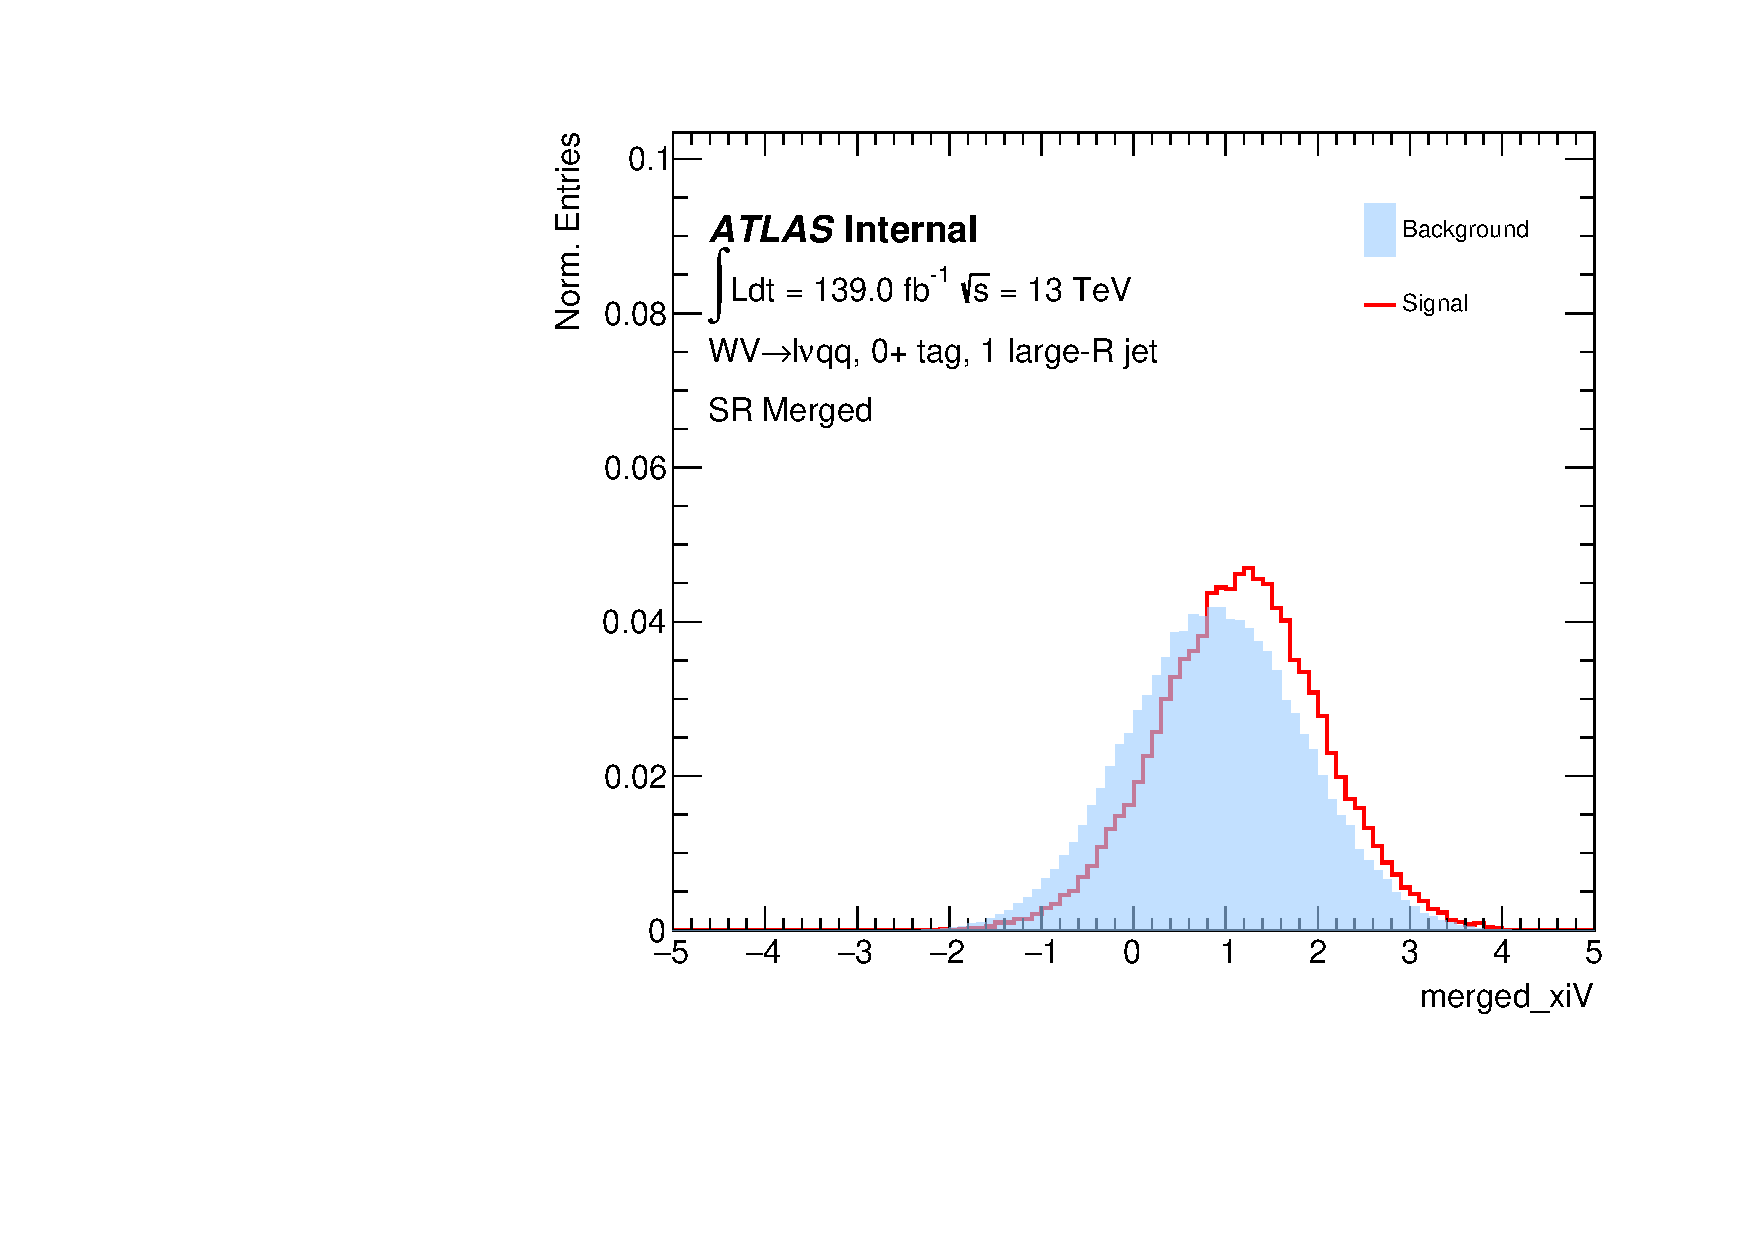
\includegraphics[width=0.3\textwidth]{figures/ml_dnn/variables/SR_Mer/norm_plot_merged_xiV.pdf}}\quad
%%  \subfloat[]{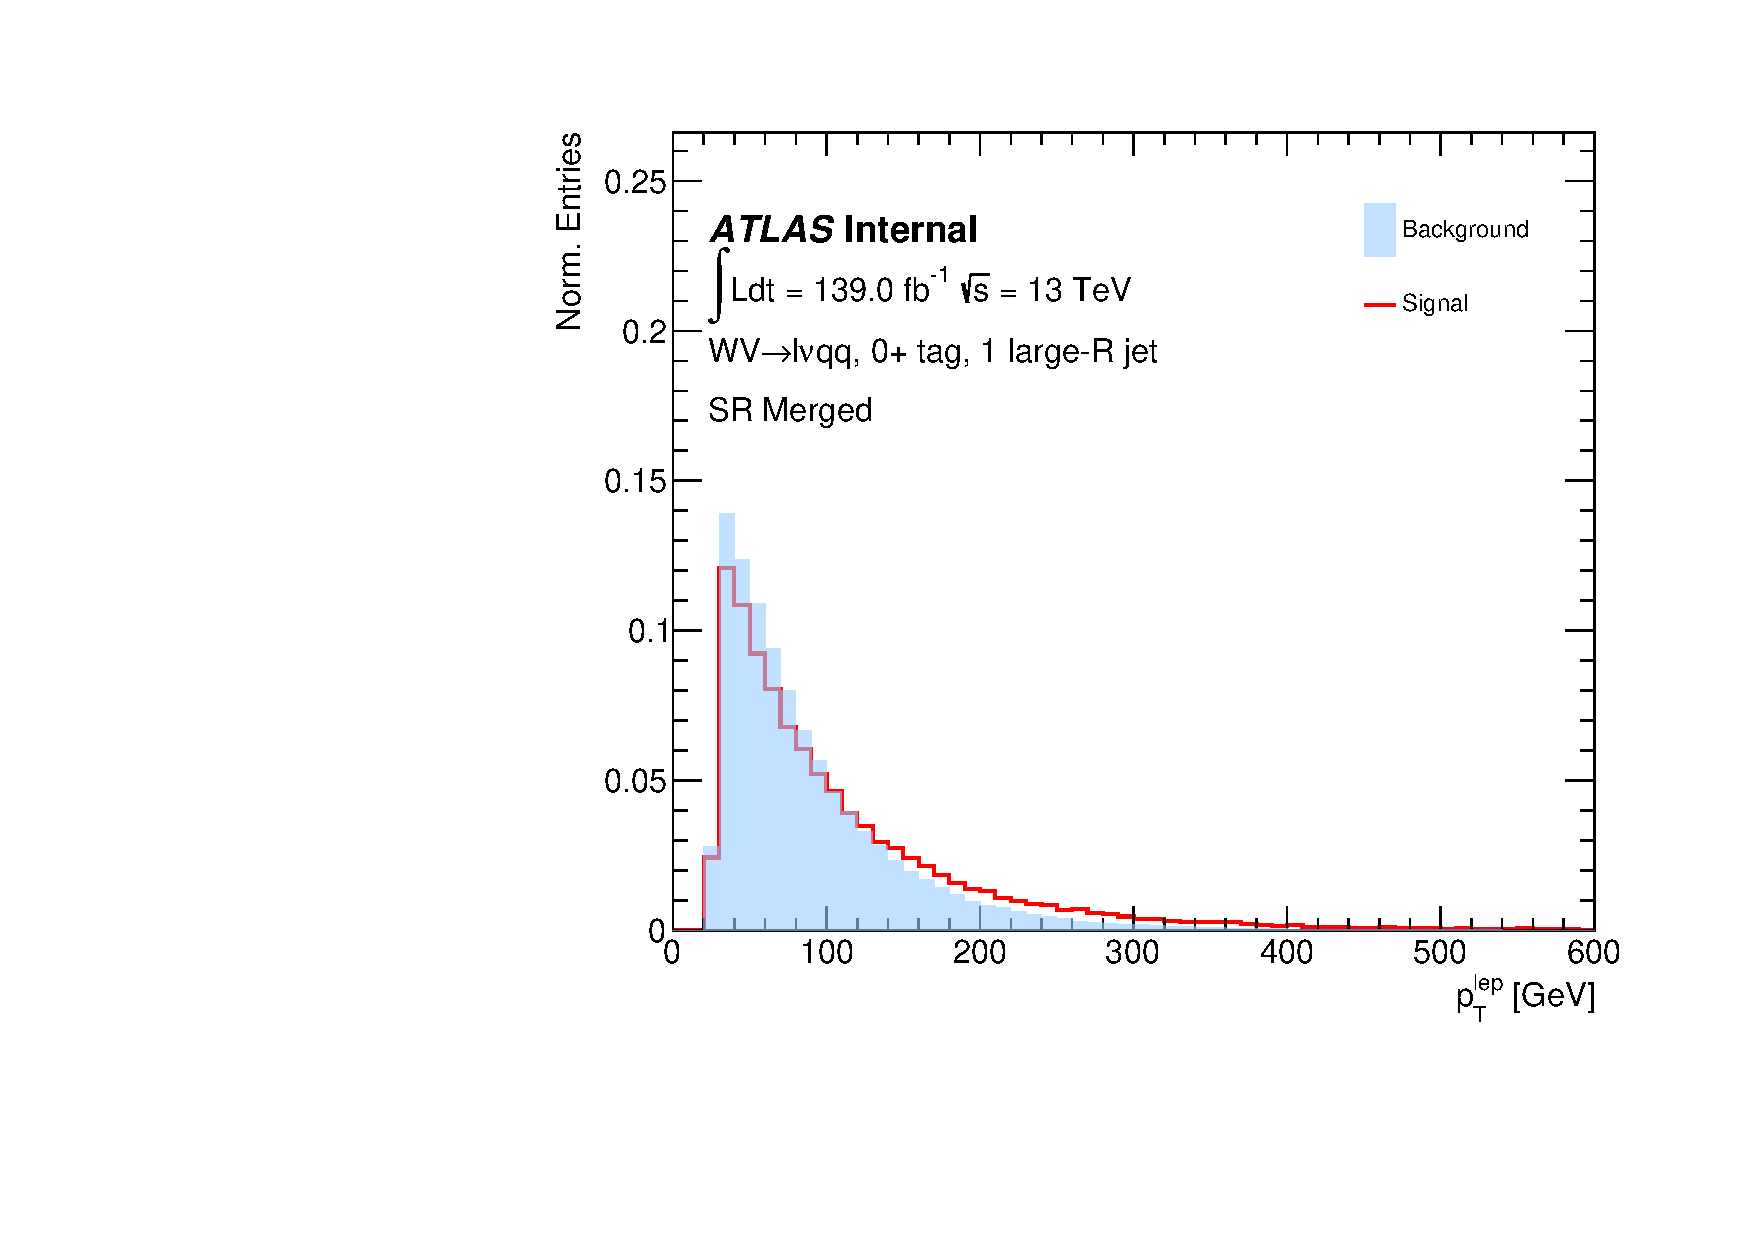
\includegraphics[width=0.3\textwidth]{figures/ml_dnn/variables/SR_Mer/norm_plot_lep_pt.pdf}}

 \caption{Distributions of input variables in the Merged SR (Continued on next page)}
 \label{fig:mer_inputs-part1}
\end{figure}

\begin{figure}[ht]
 \centering
  % Row 3
  \subfloat[]{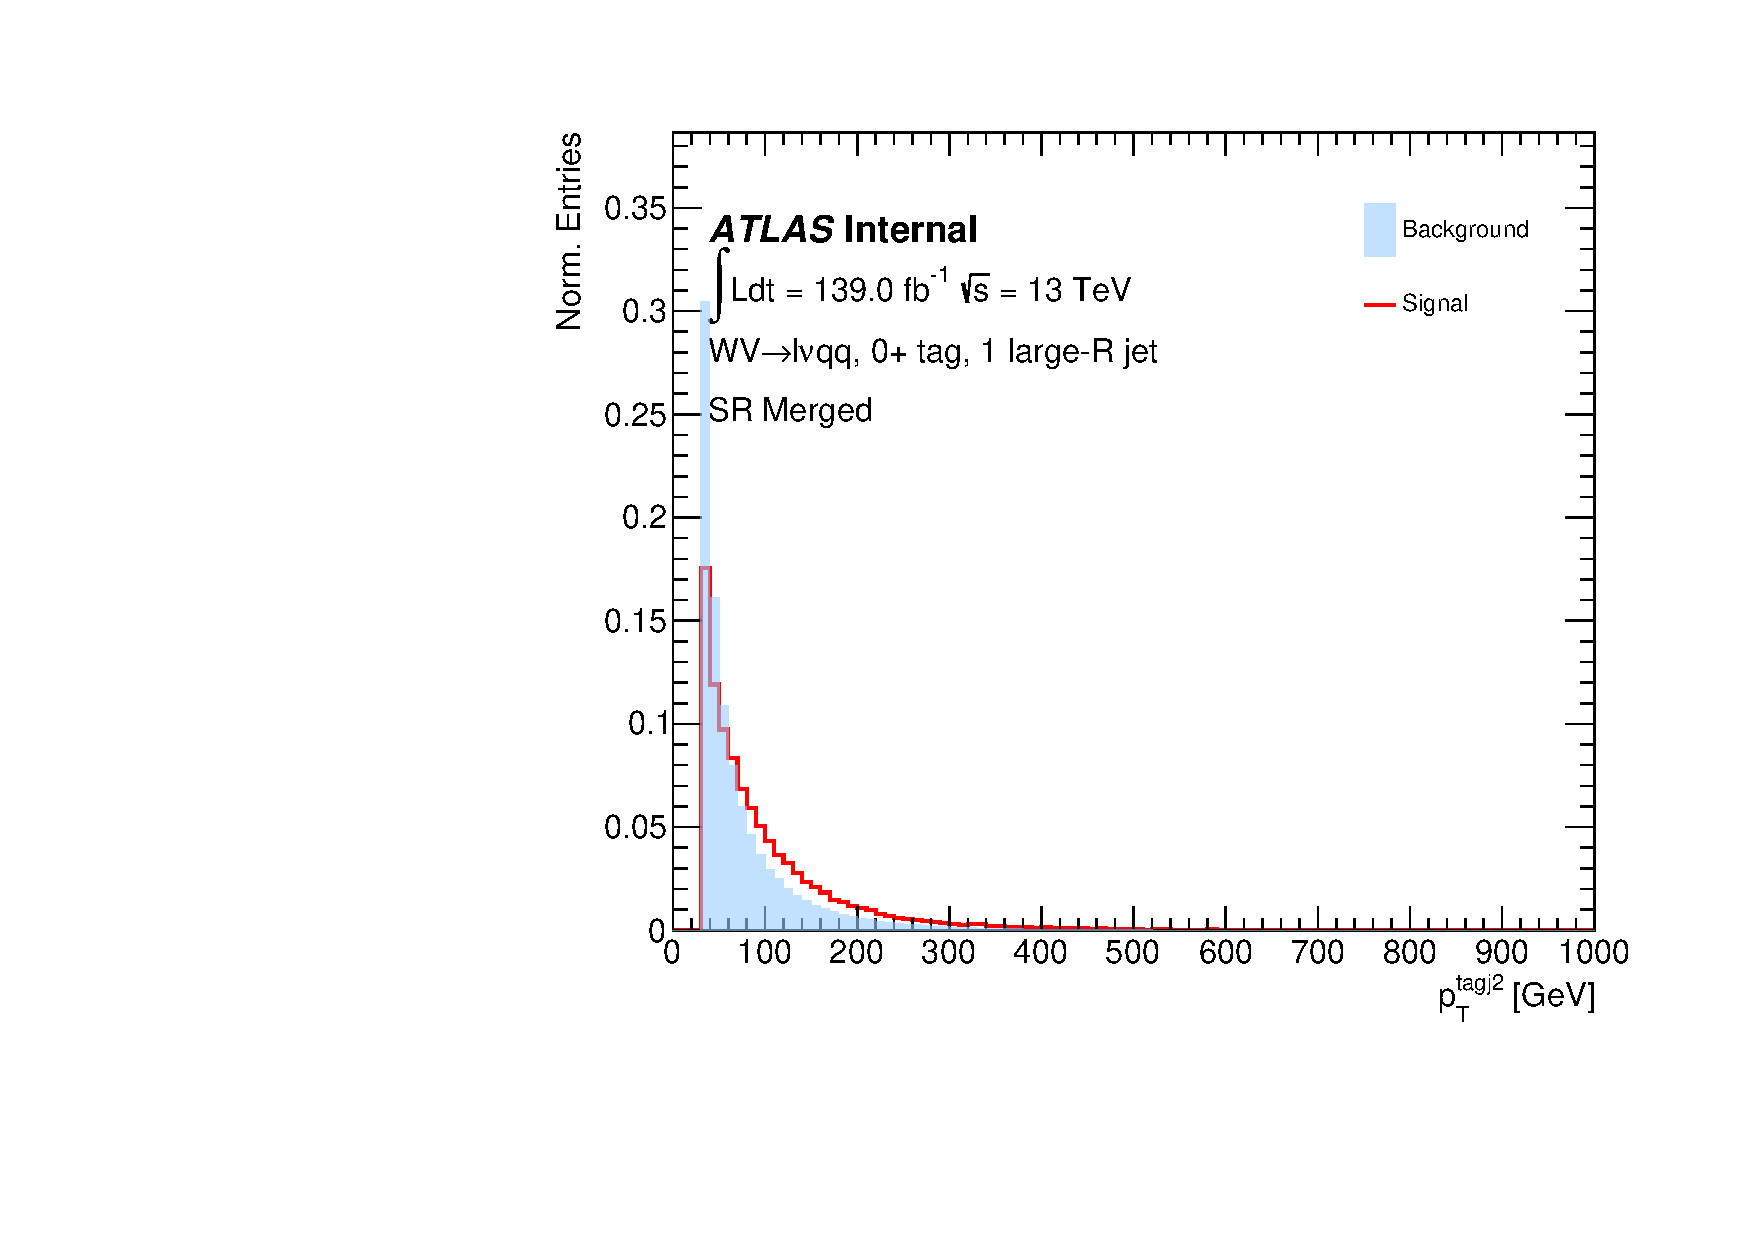
\includegraphics[width=0.3\textwidth]{figures/ml_dnn/variables/SR_Mer/norm_plot_merged_tagJ2_pt.pdf}}\quad
  \subfloat[]{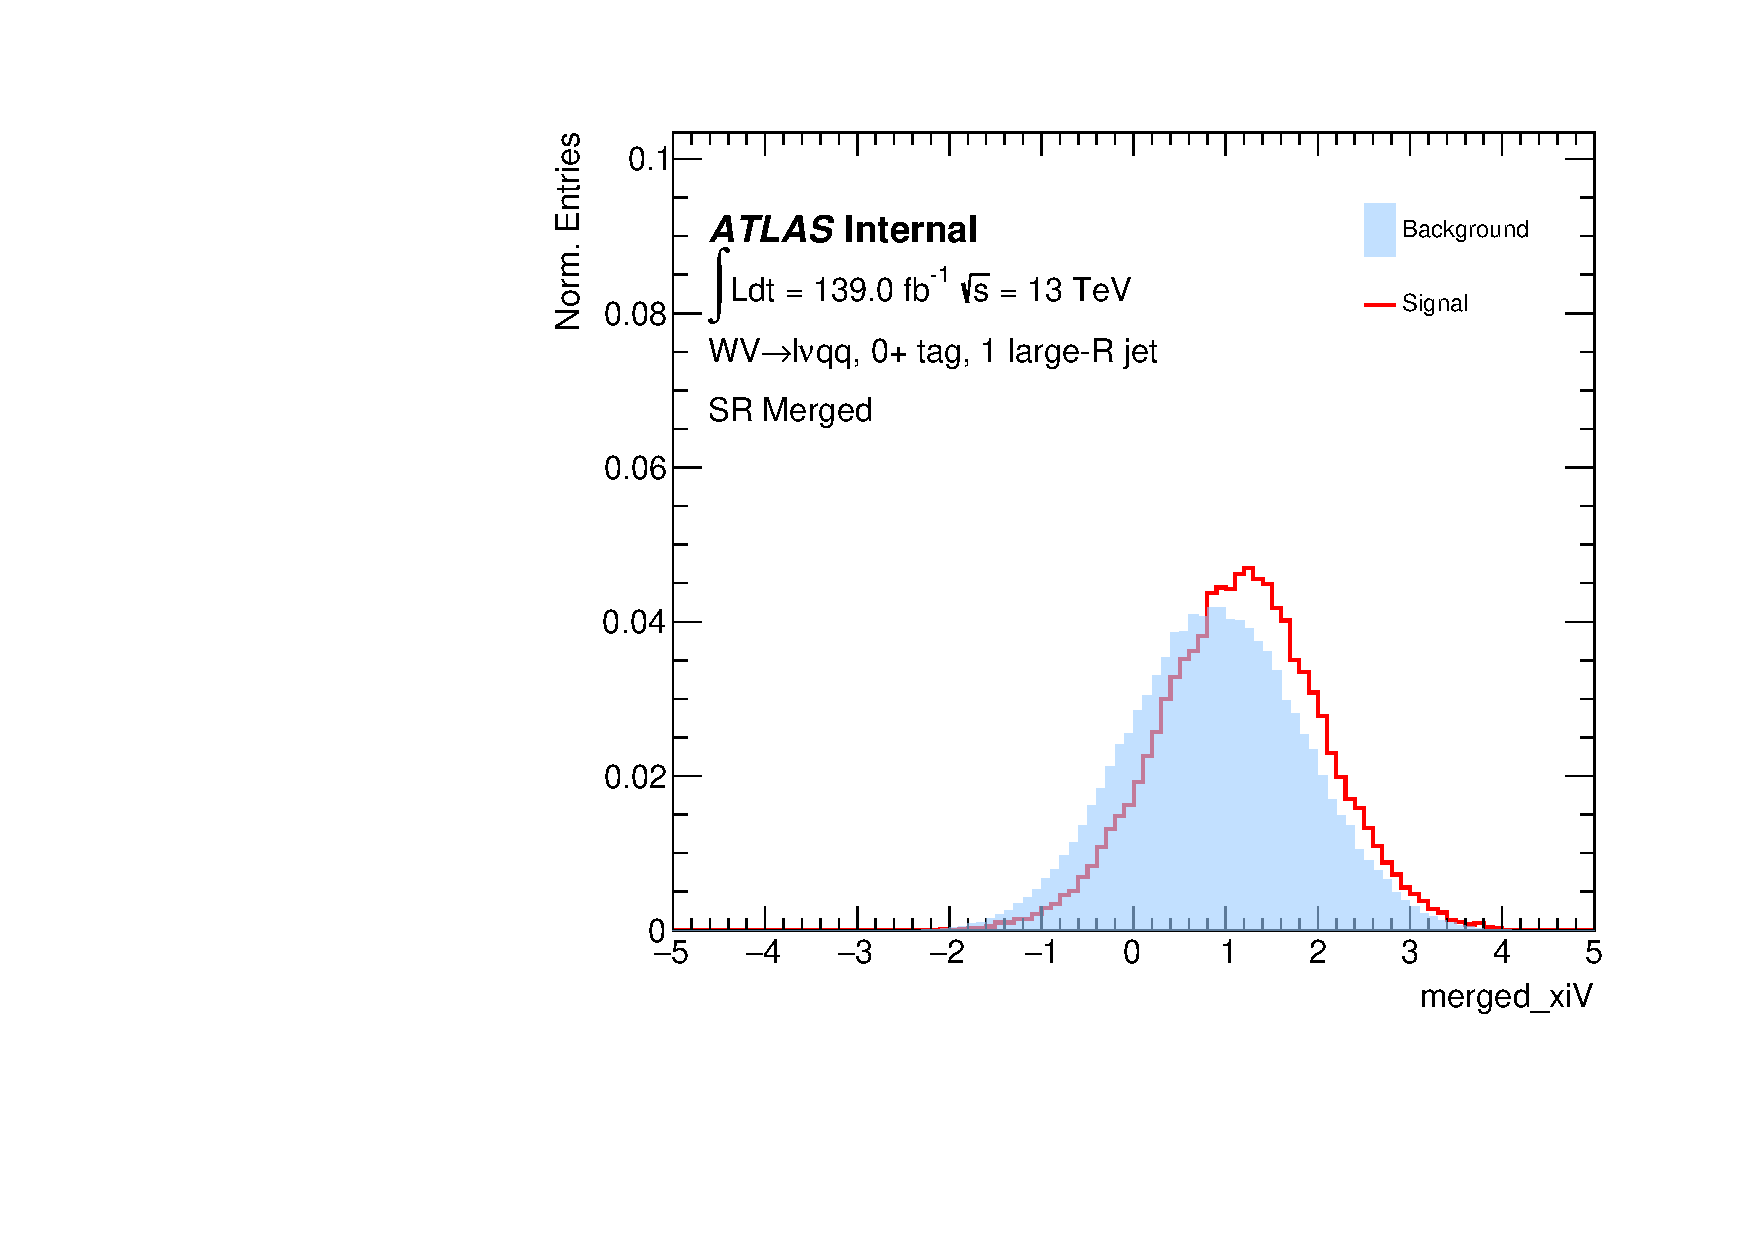
\includegraphics[width=0.3\textwidth]{figures/ml_dnn/variables/SR_Mer/norm_plot_merged_xiV.pdf}}\quad
  \subfloat[]{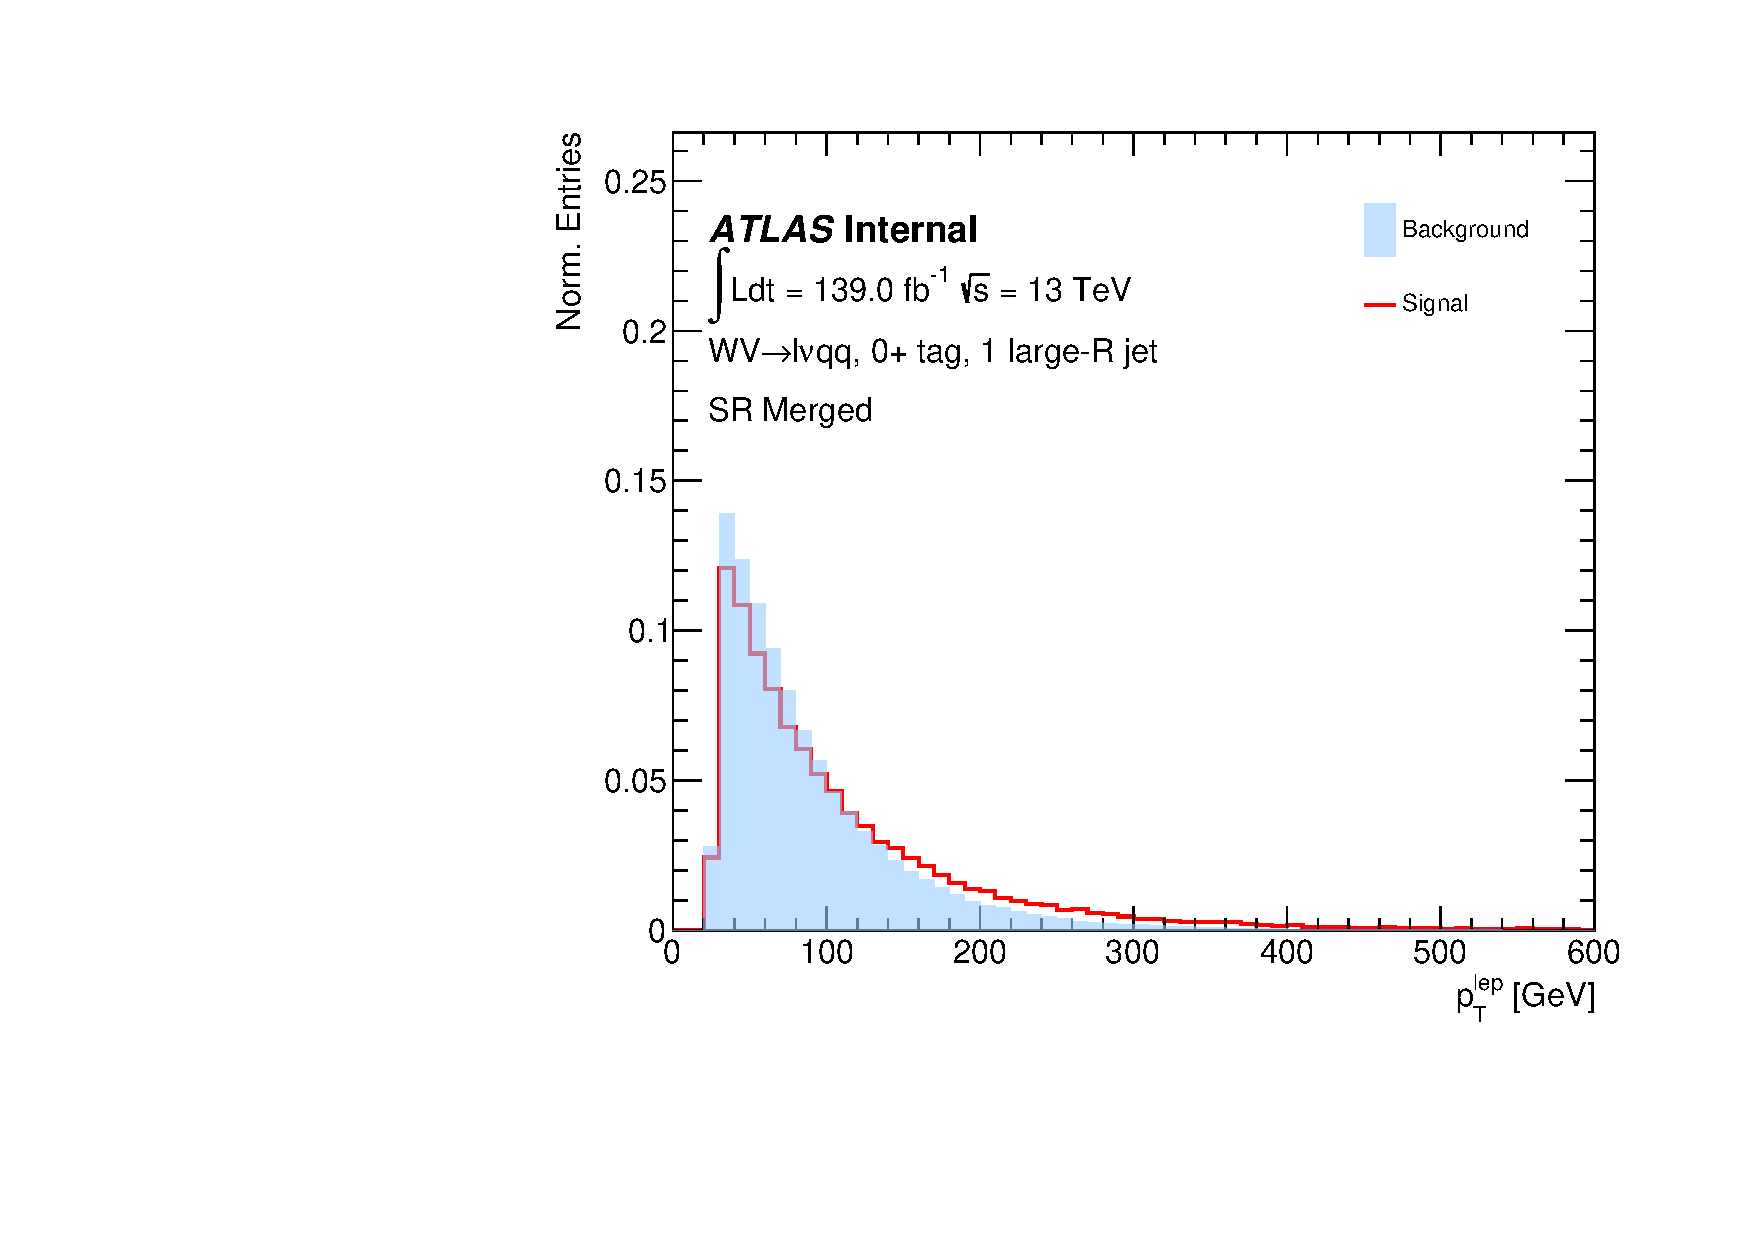
\includegraphics[width=0.3\textwidth]{figures/ml_dnn/variables/SR_Mer/norm_plot_lep_pt.pdf}}

  % Row 4
  \subfloat[]{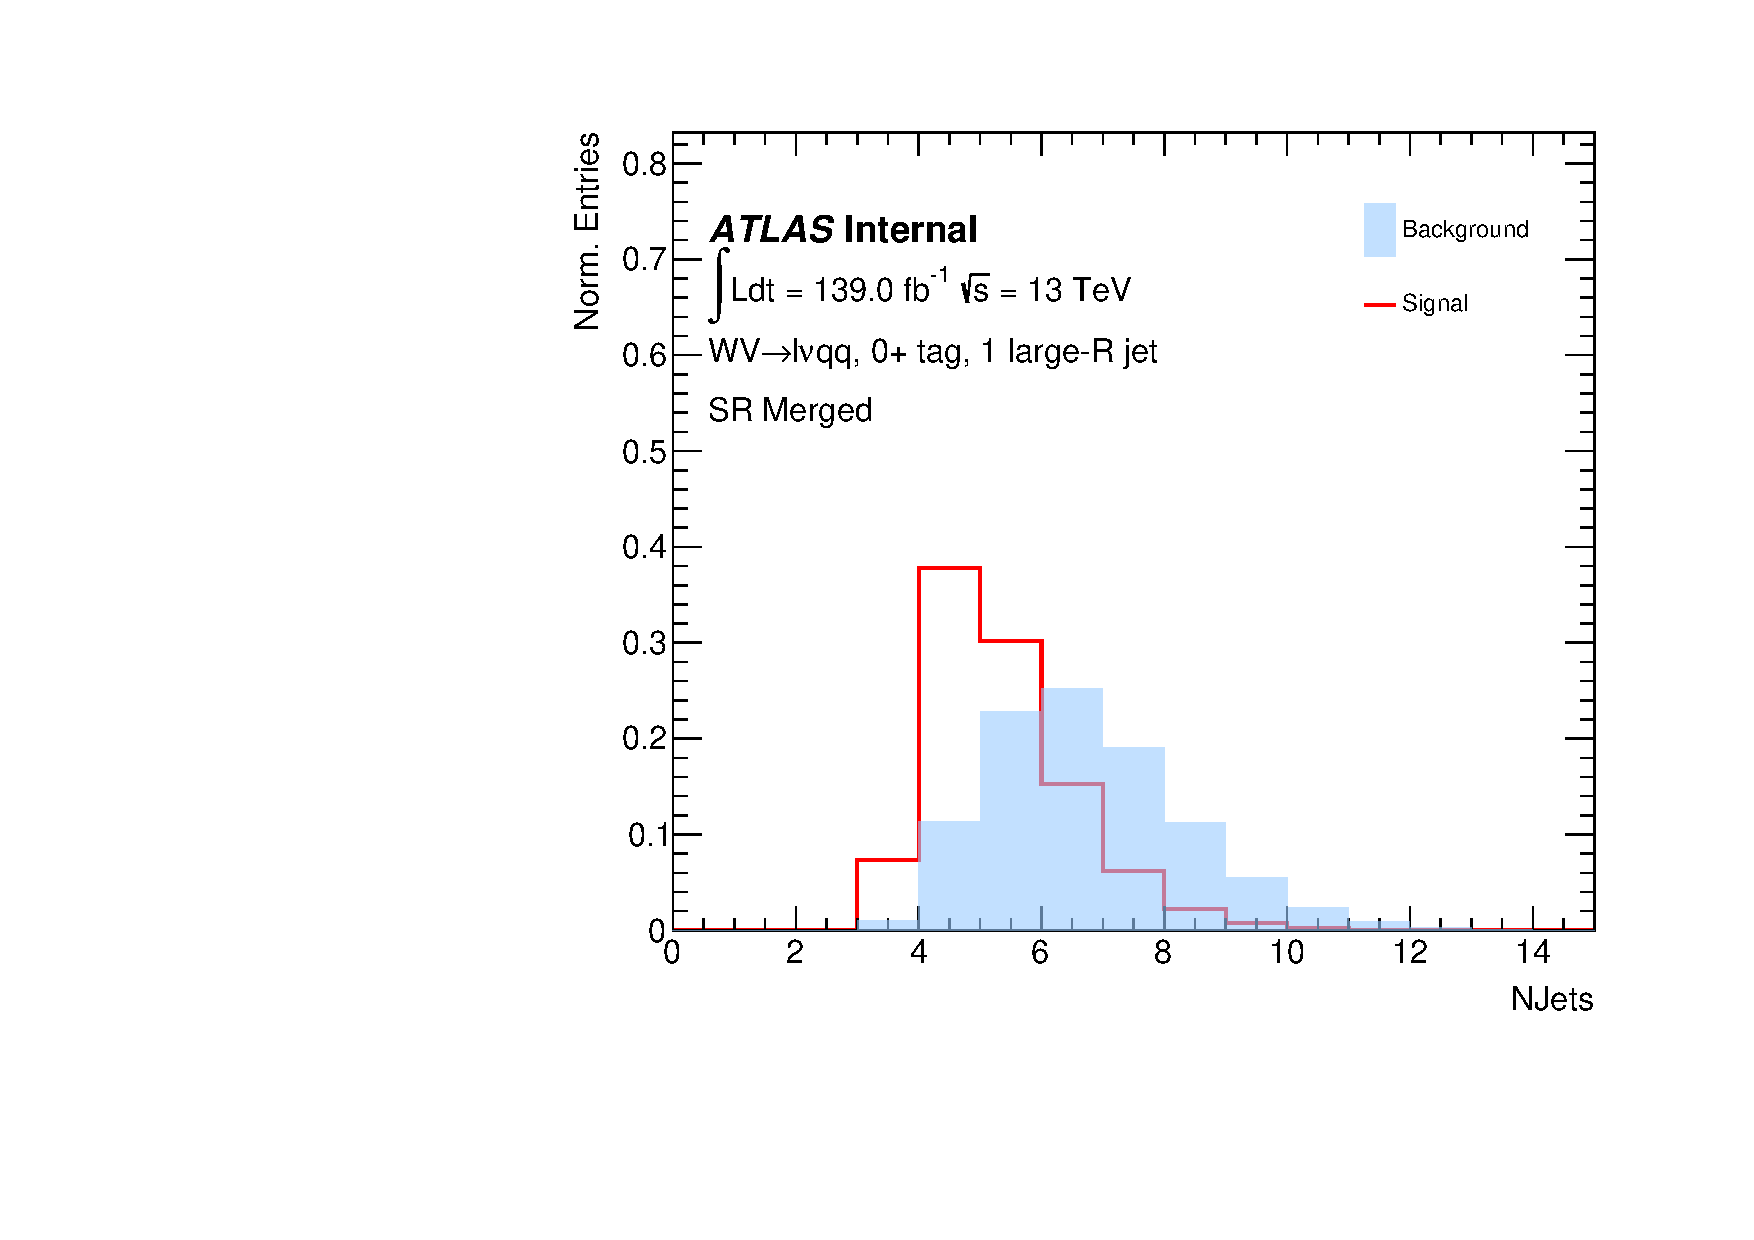
\includegraphics[width=0.3\textwidth]{figures/ml_dnn/variables/SR_Mer/norm_plot_NJets.pdf}}\quad
  \subfloat[]{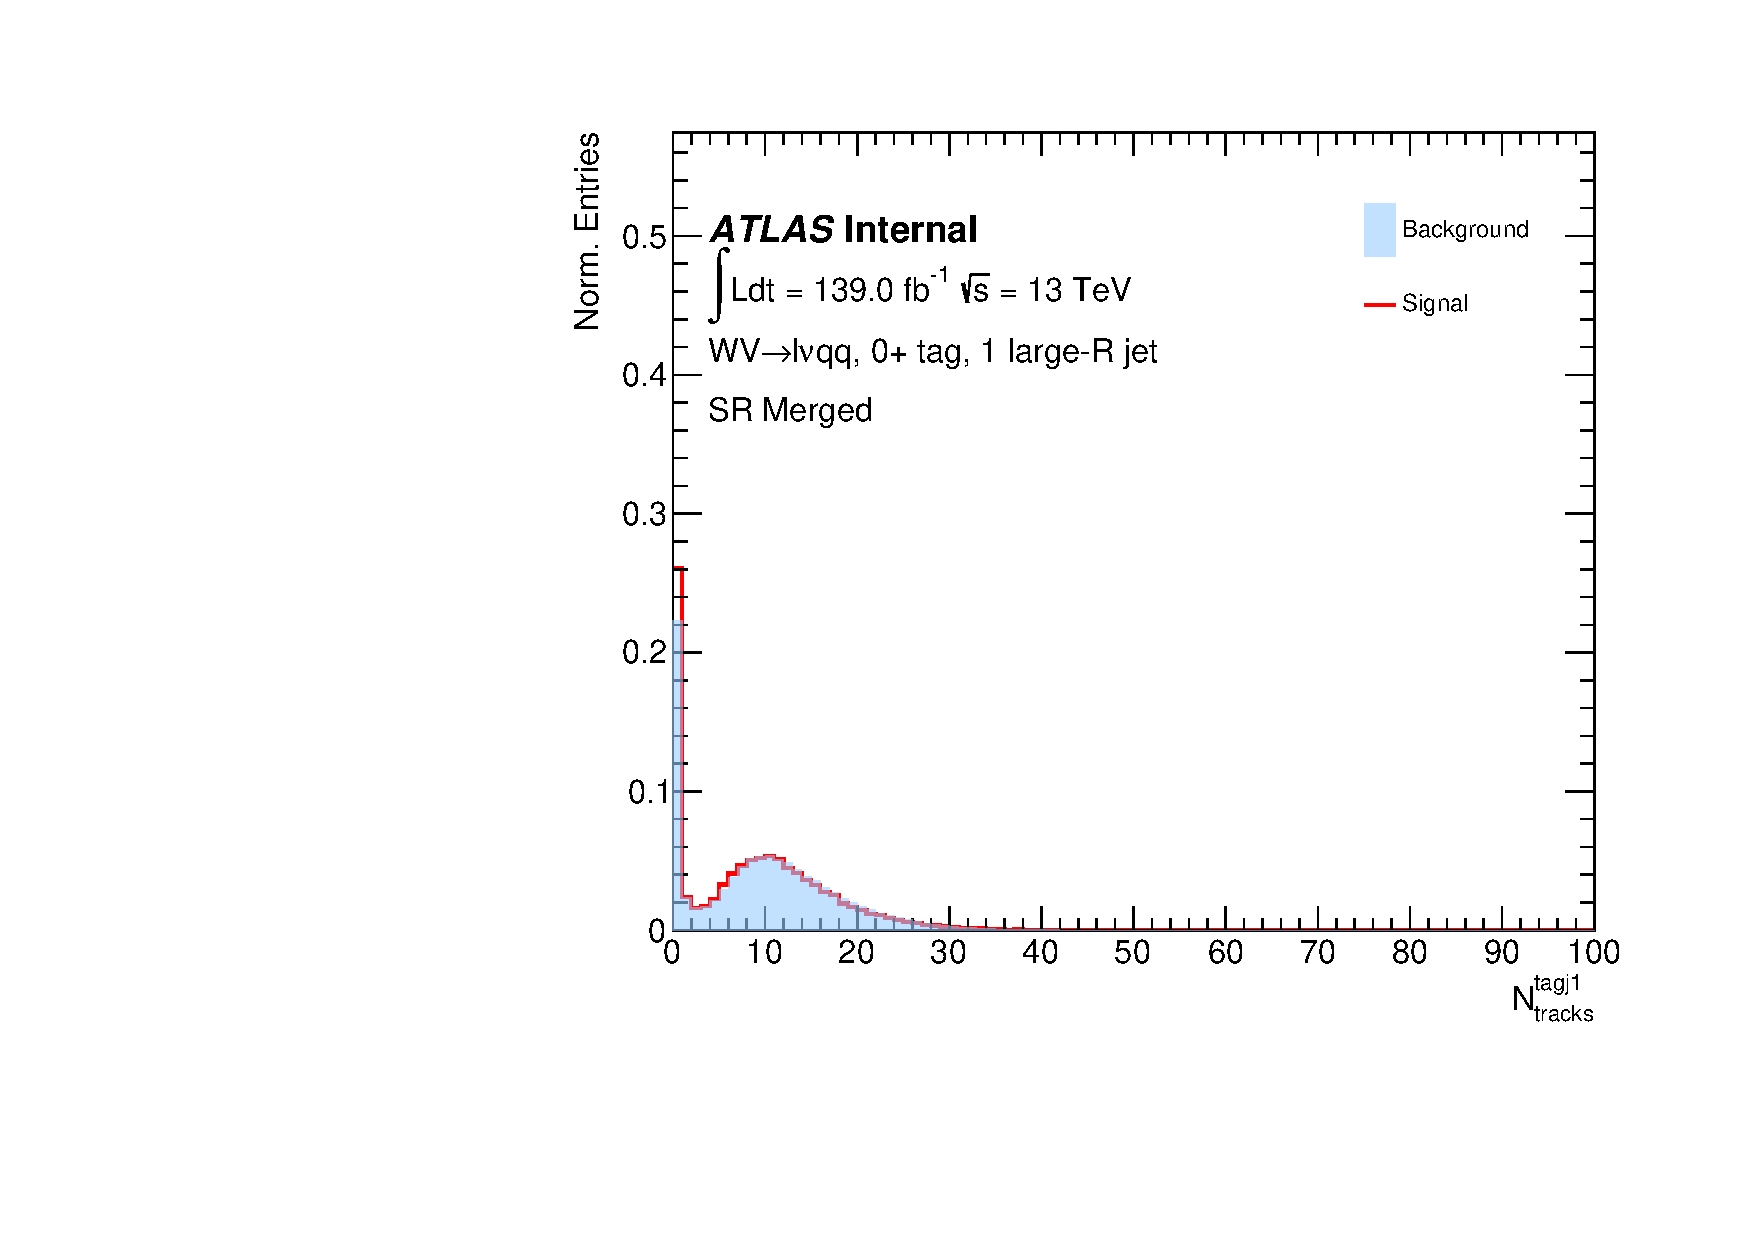
\includegraphics[width=0.3\textwidth]{figures/ml_dnn/variables/SR_Mer/norm_plot_merged_tagJ1_nTracks.pdf}}\quad
  \subfloat[]{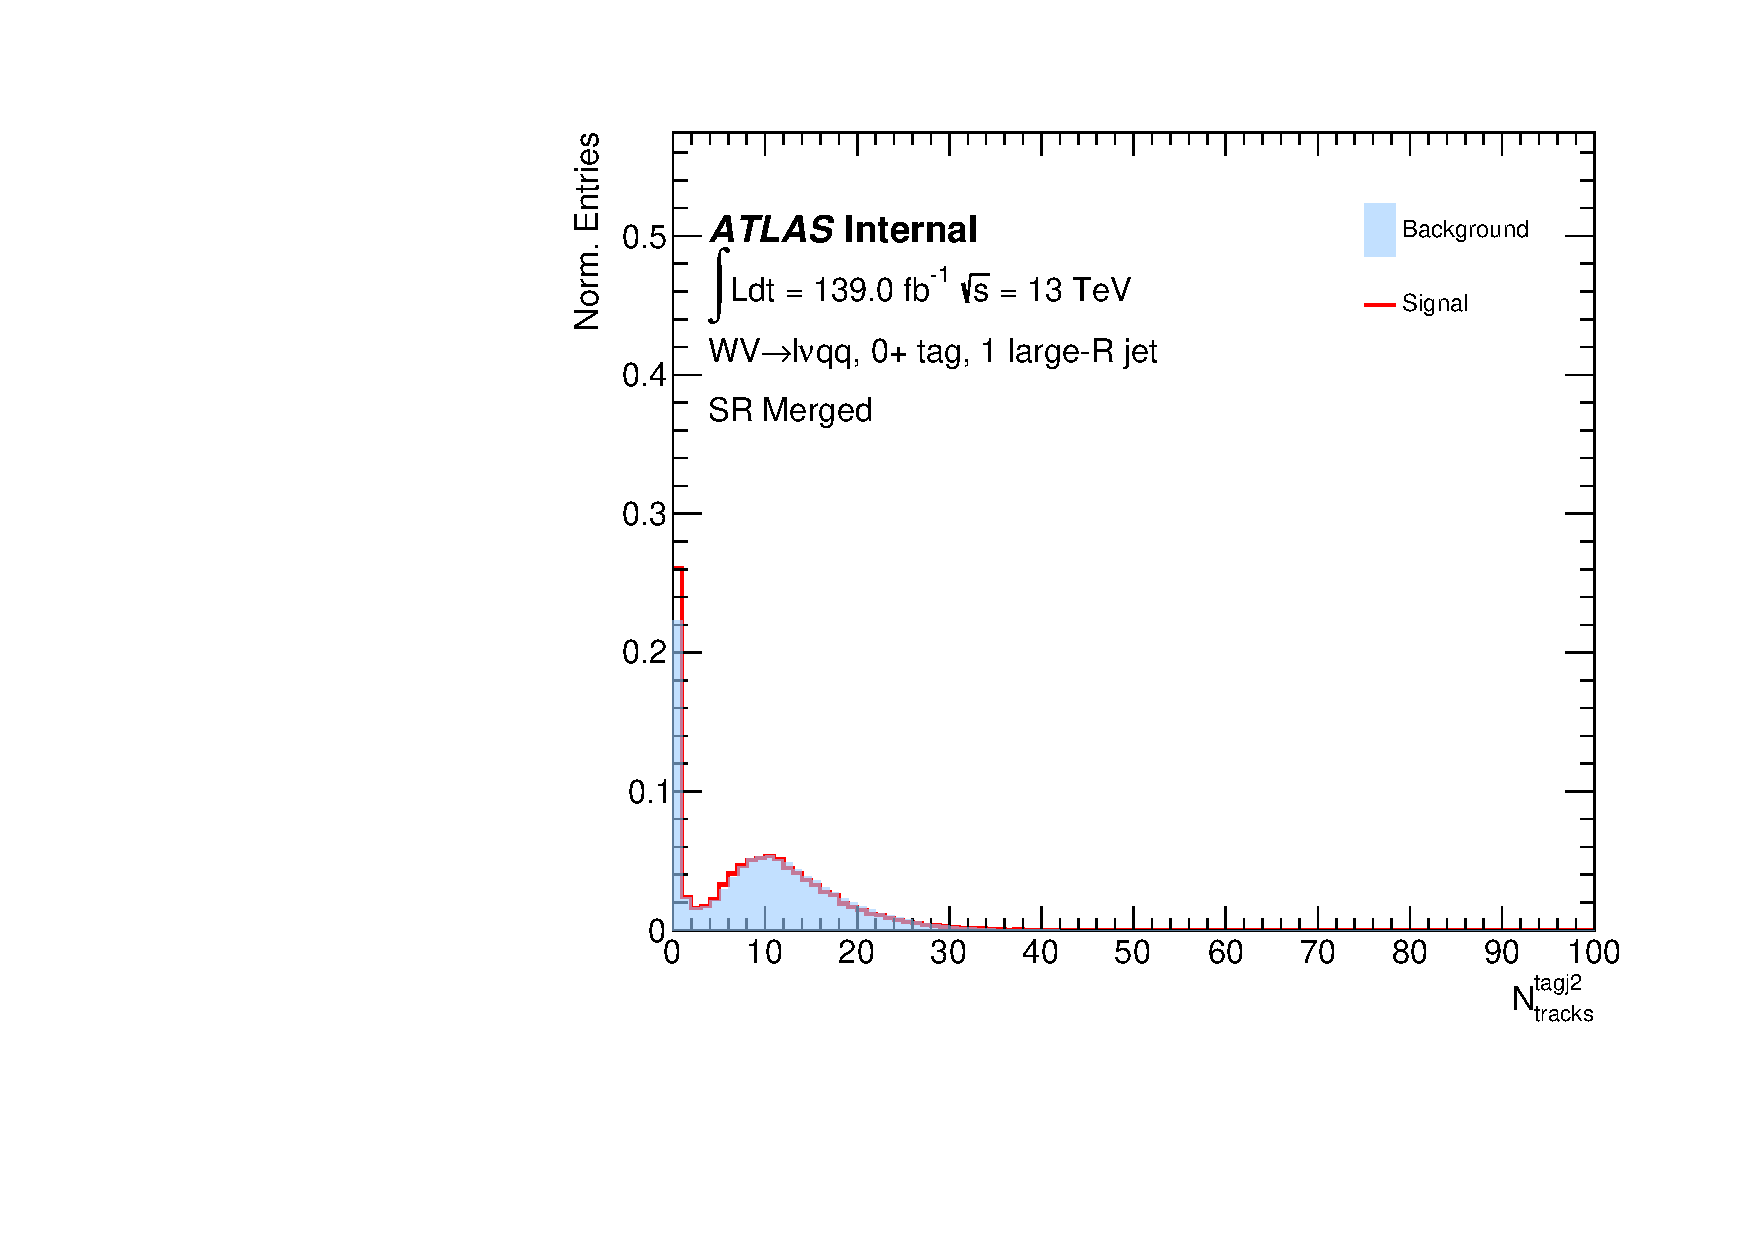
\includegraphics[width=0.3\textwidth]{figures/ml_dnn/variables/SR_Mer/norm_plot_merged_tagJ2_nTracks.pdf}}

  % Row 5
  \subfloat[]{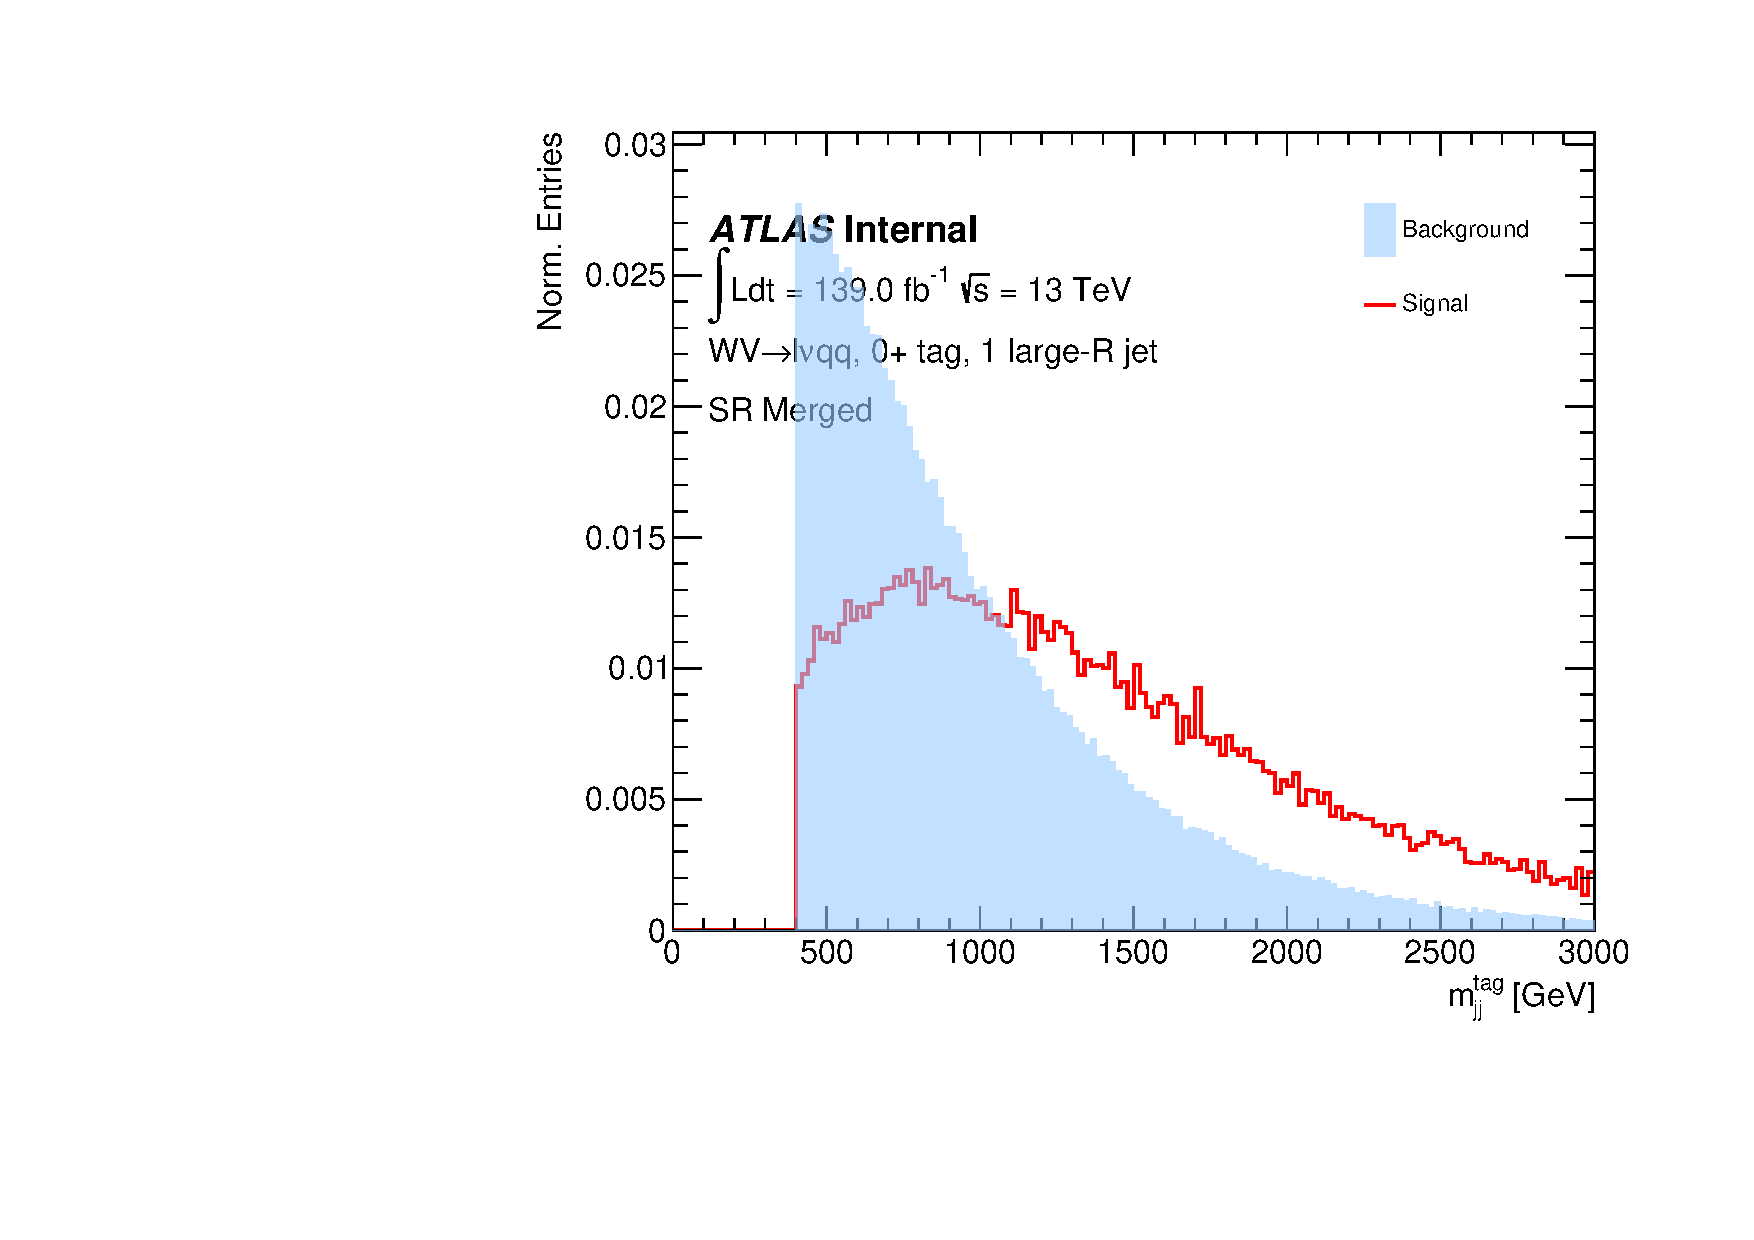
\includegraphics[width=0.3\textwidth]{figures/ml_dnn/variables/SR_Mer/norm_plot_merged_tagMjj.pdf}}\quad
  \subfloat[]{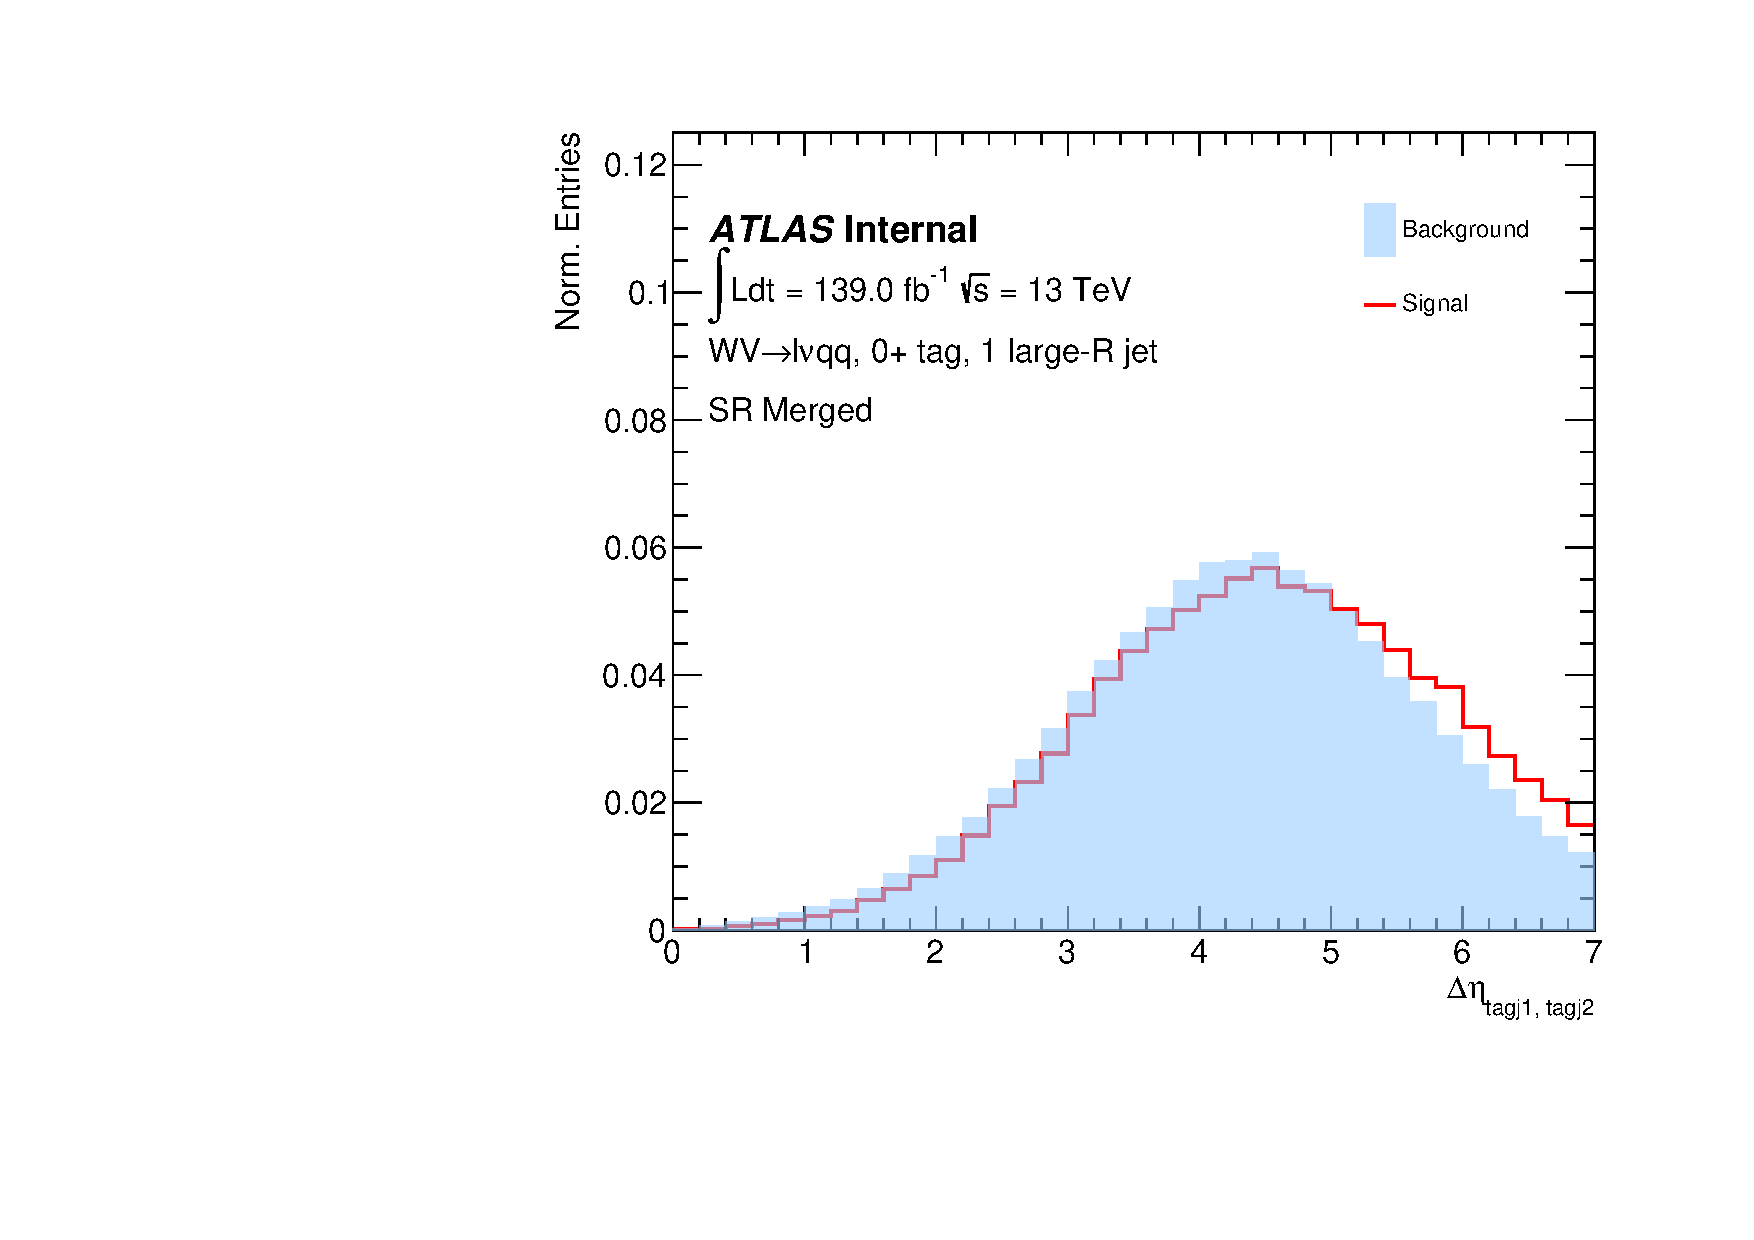
\includegraphics[width=0.3\textwidth]{figures/ml_dnn/variables/SR_Mer/norm_plot_merged_tagJdEta.pdf}}\quad
  \subfloat[]{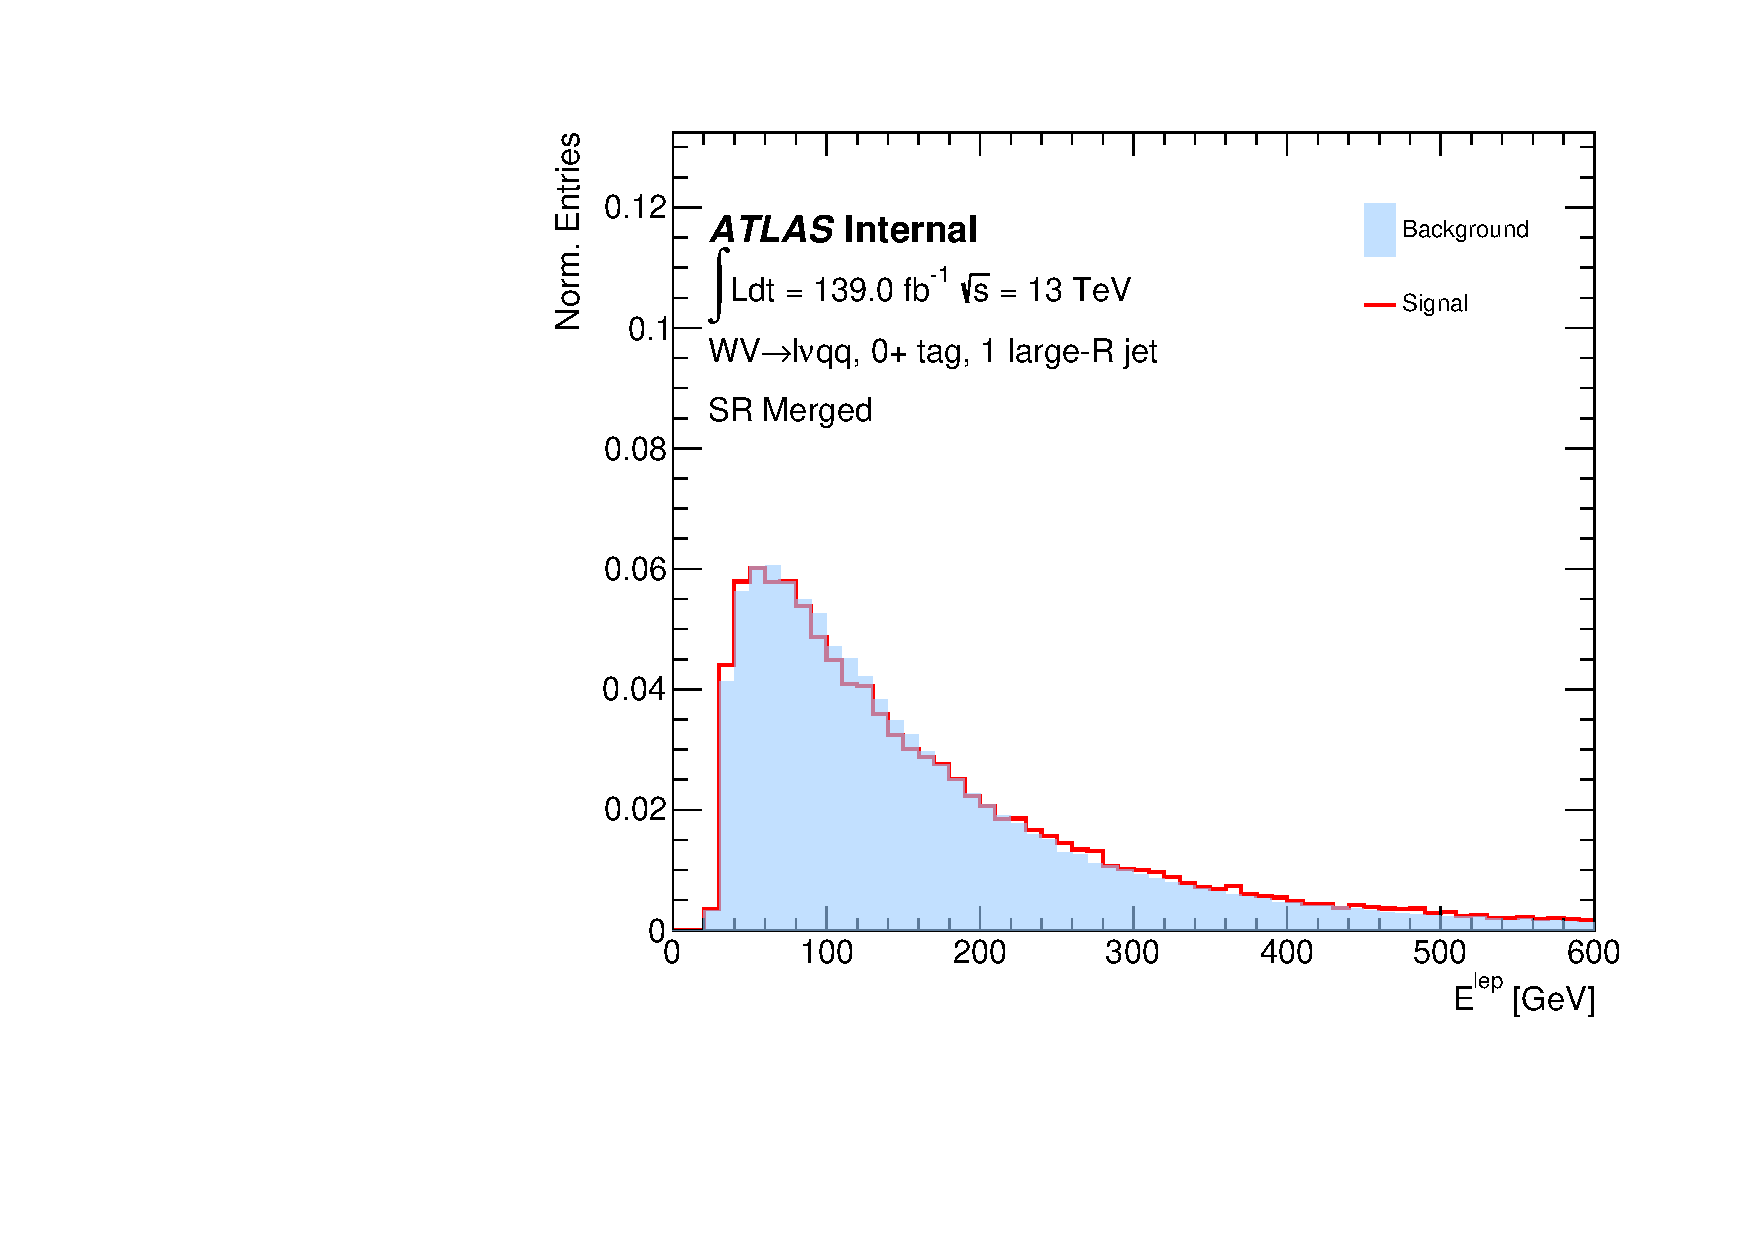
\includegraphics[width=0.3\textwidth]{figures/ml_dnn/variables/SR_Mer/norm_plot_lep_e.pdf}}

 \caption{Distributions of input variables in the Merged SR (Continued)}
 \label{fig:mer_inputs-part2}
\end{figure}

\begin{figure}[ht]
 \centering
  % Row 1
  \subfloat[]{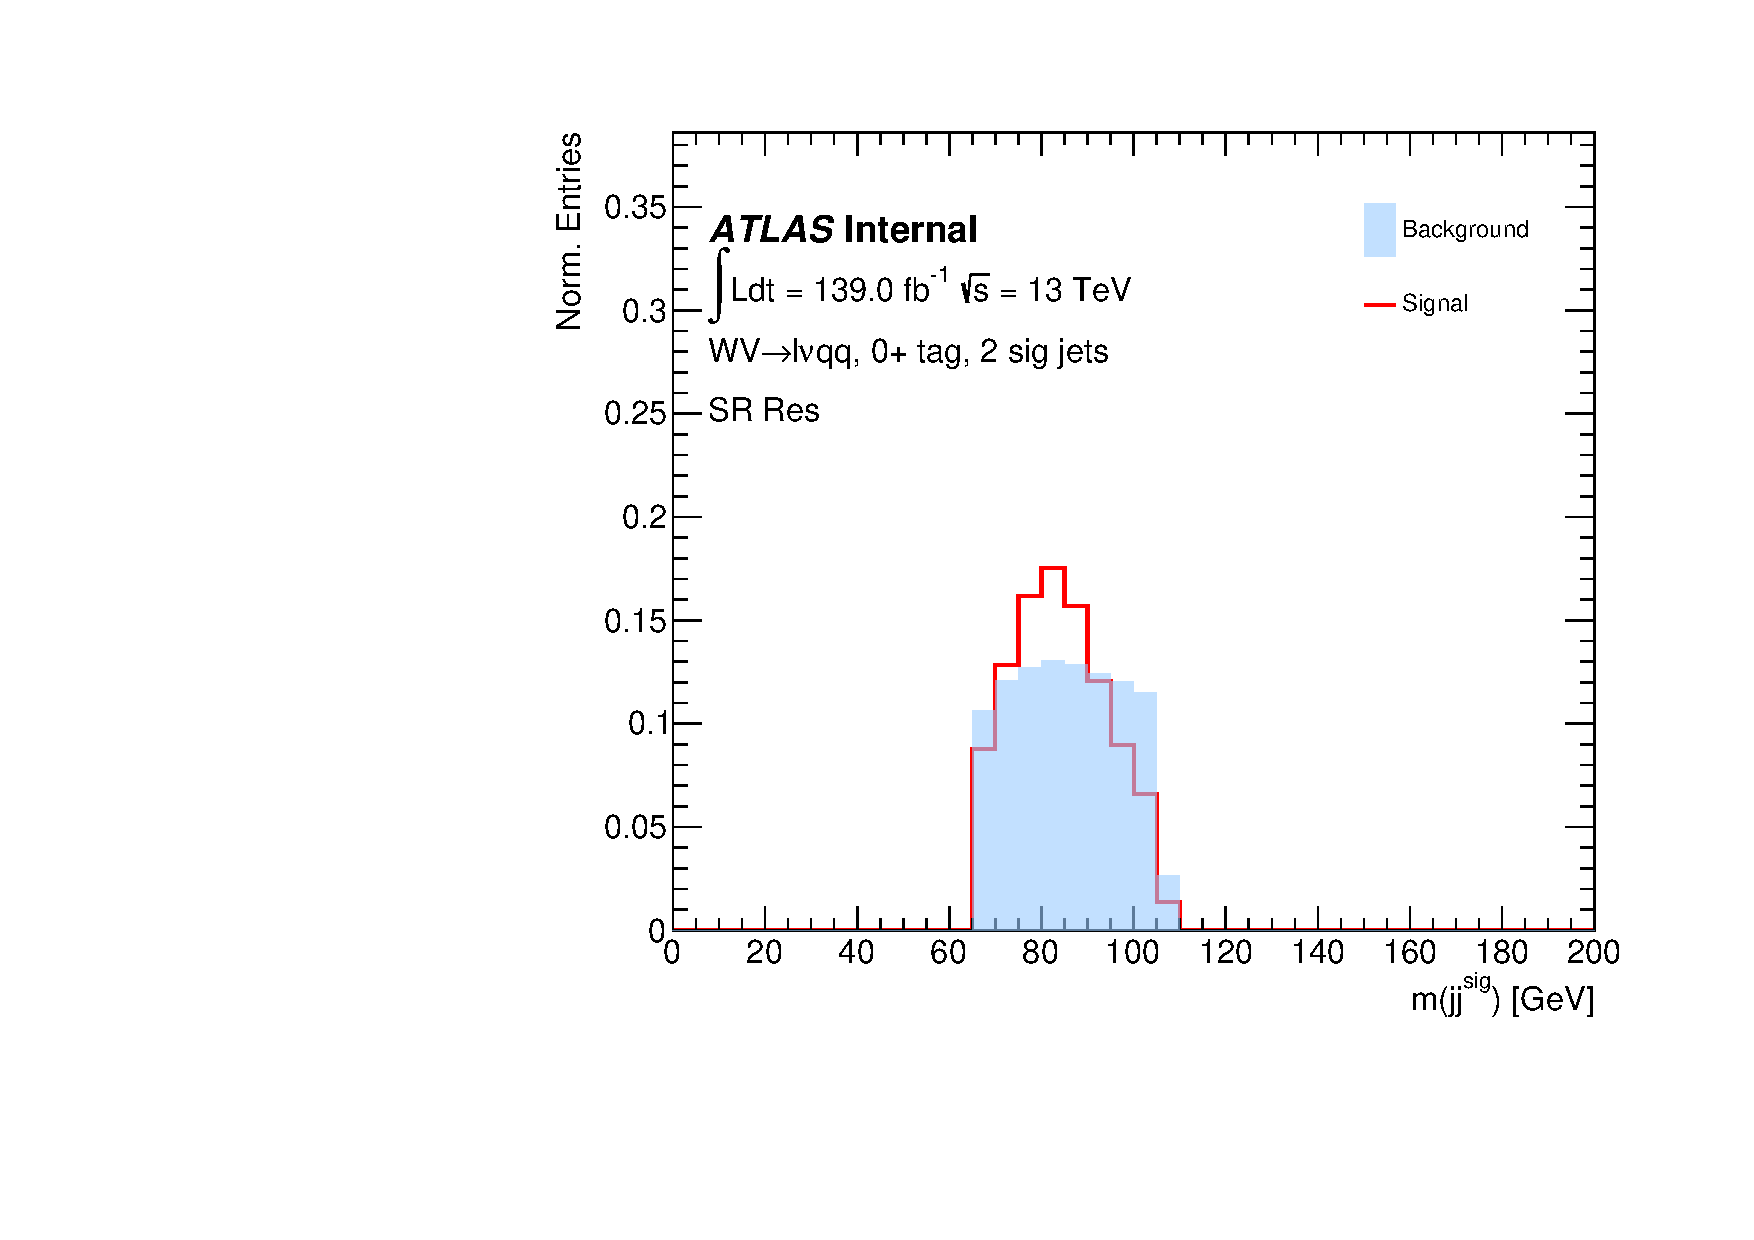
\includegraphics[width=0.3\textwidth]{figures/ml_dnn/variables/SR_Res/norm_plot_Dijet_m.pdf}}\quad
  \subfloat[]{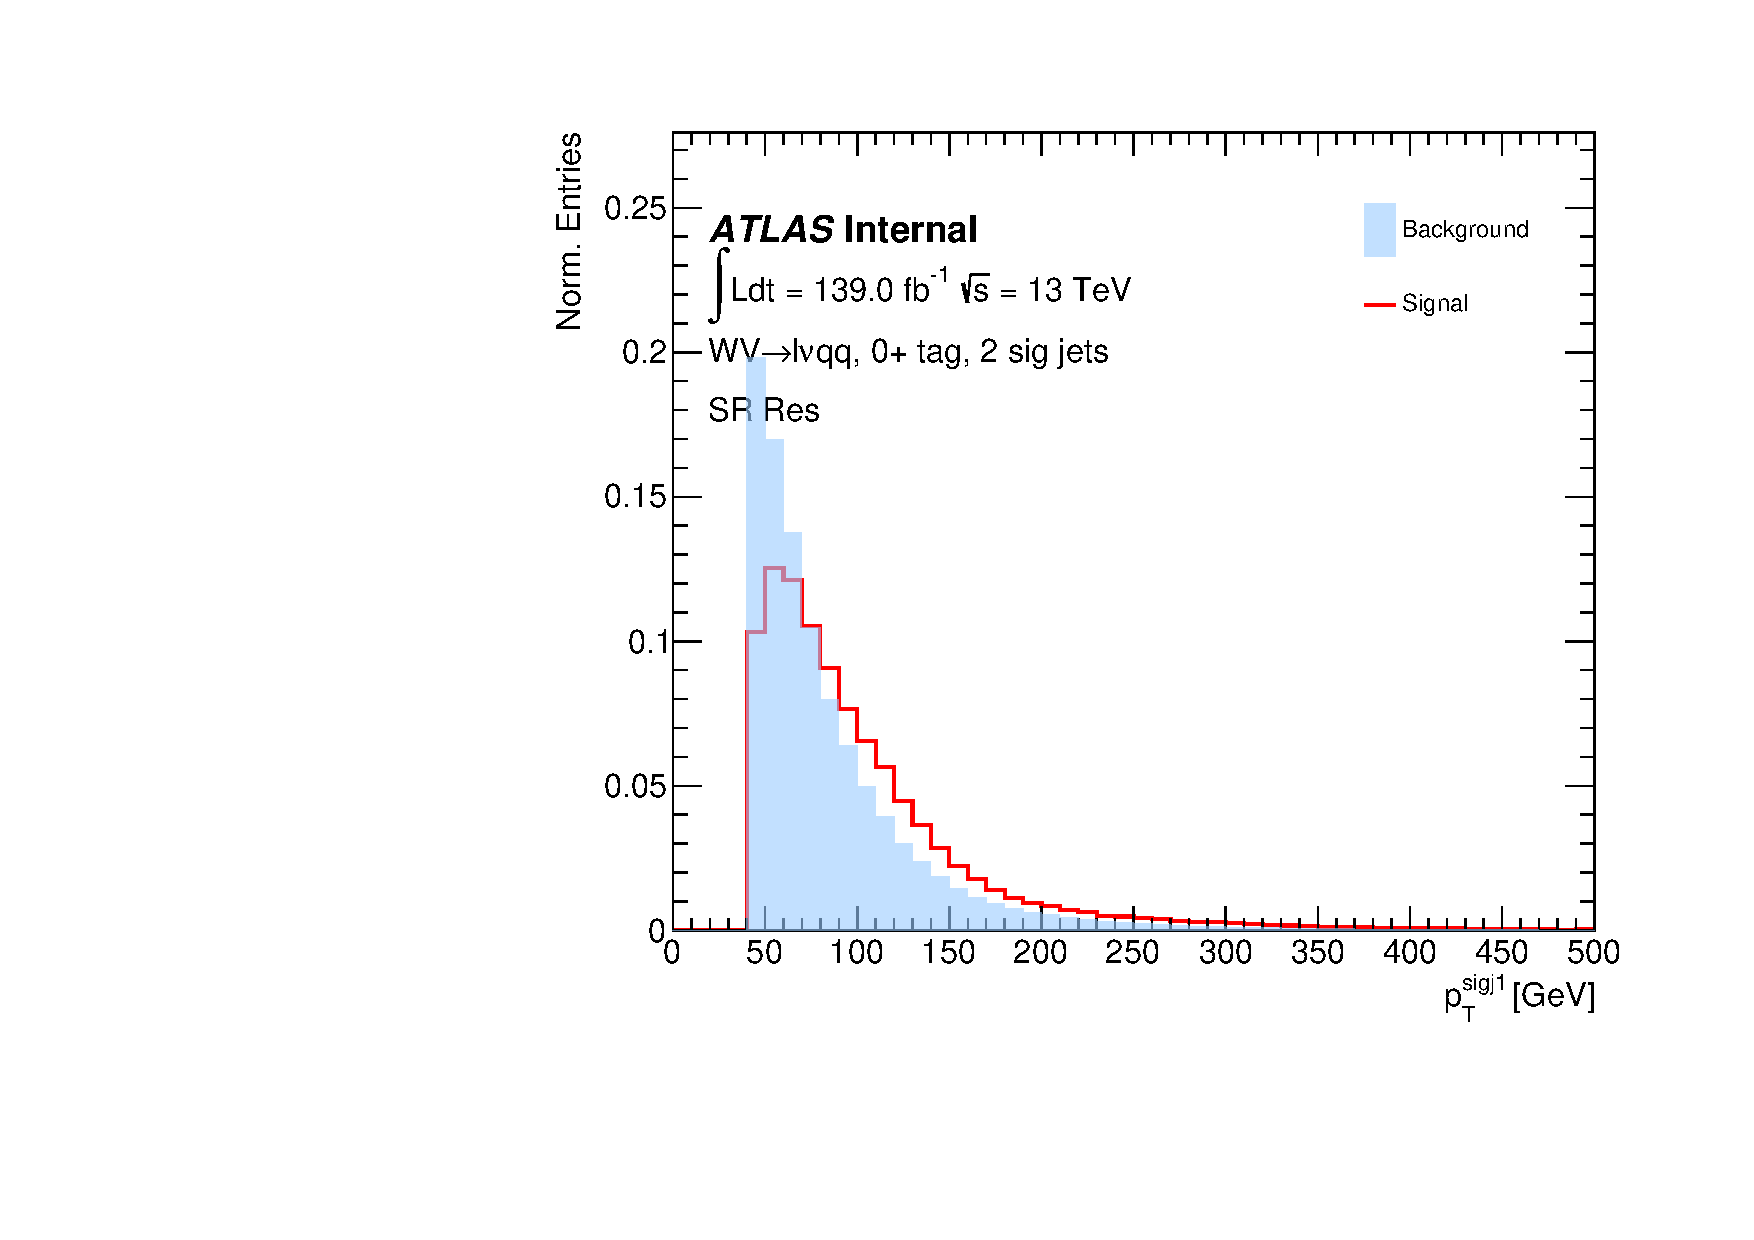
\includegraphics[width=0.3\textwidth]{figures/ml_dnn/variables/SR_Res/norm_plot_sigJ1_pt.pdf}}\quad
  \subfloat[]{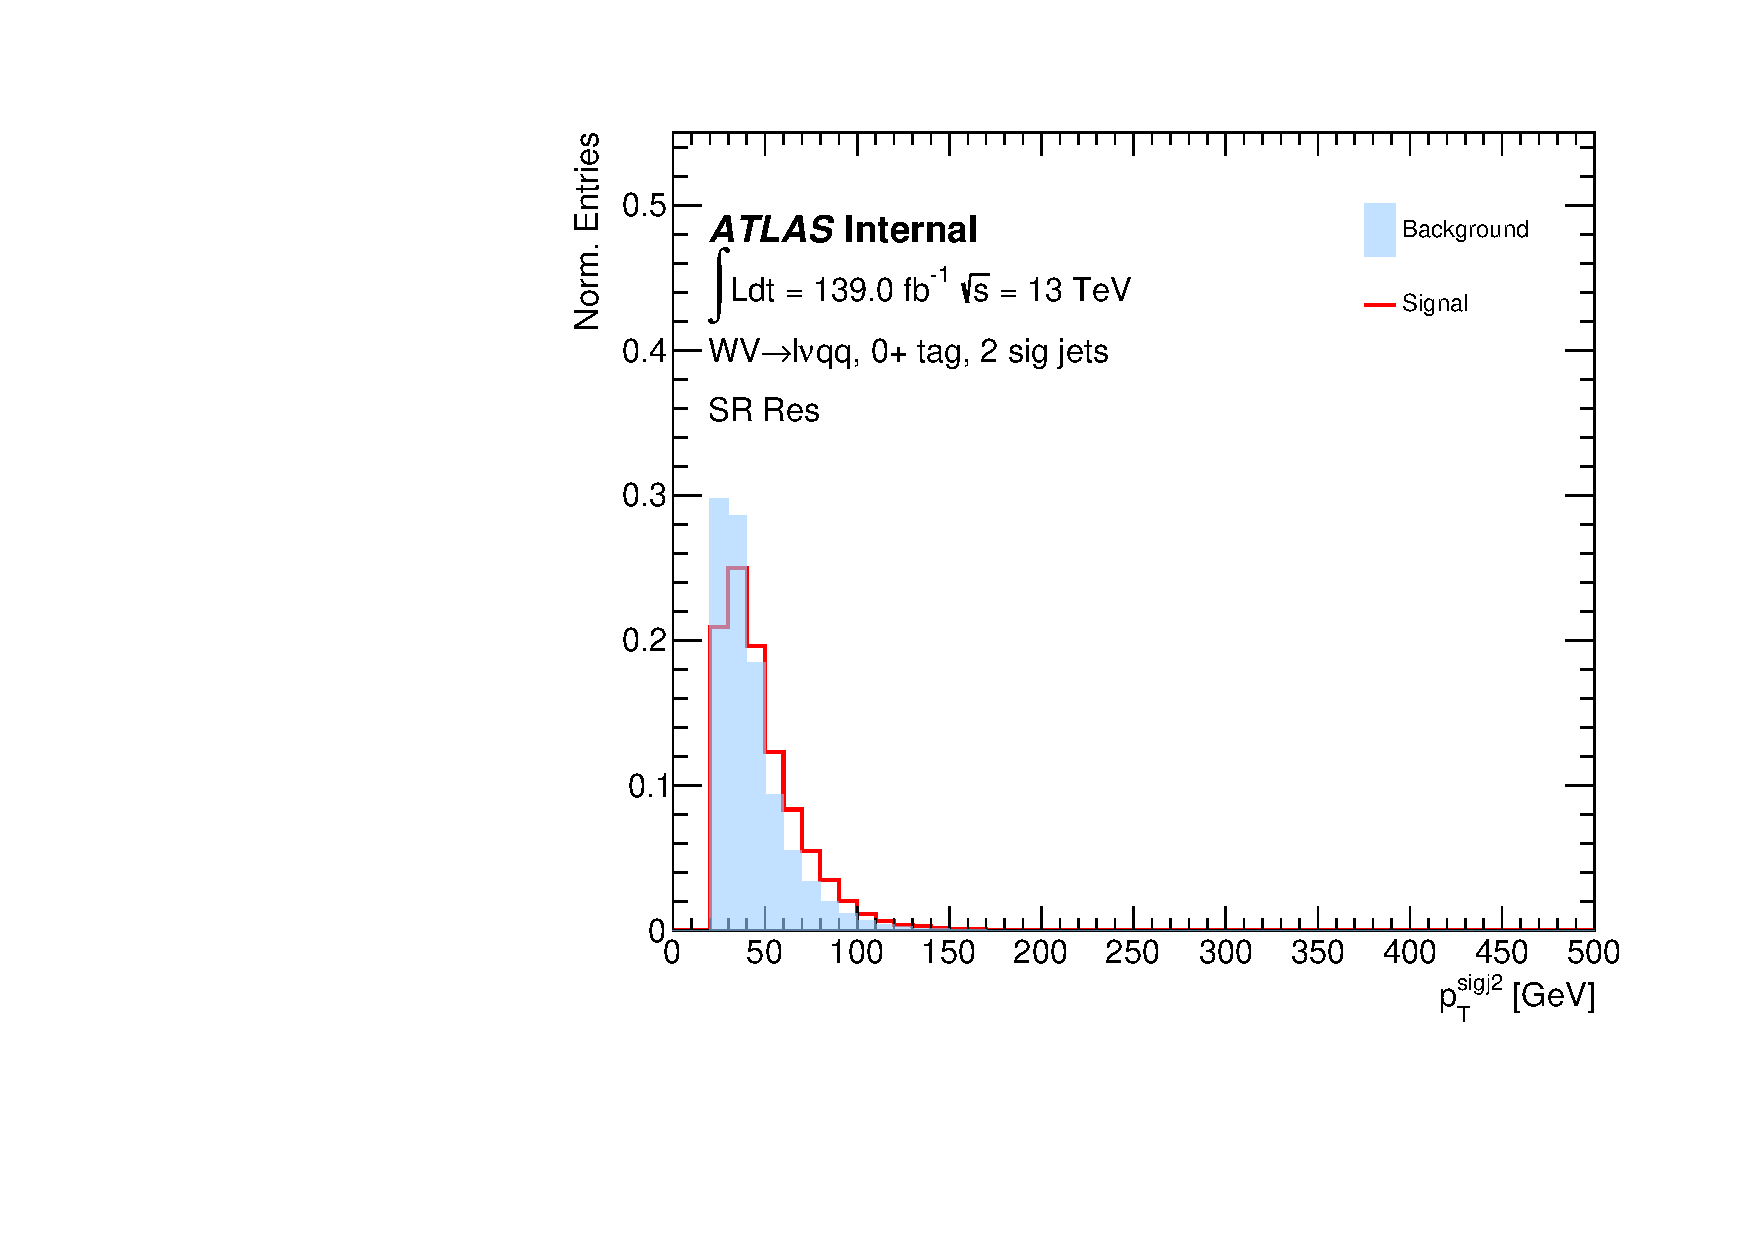
\includegraphics[width=0.3\textwidth]{figures/ml_dnn/variables/SR_Res/norm_plot_sigJ2_pt.pdf}}
  
  % Row 2
  \subfloat[]{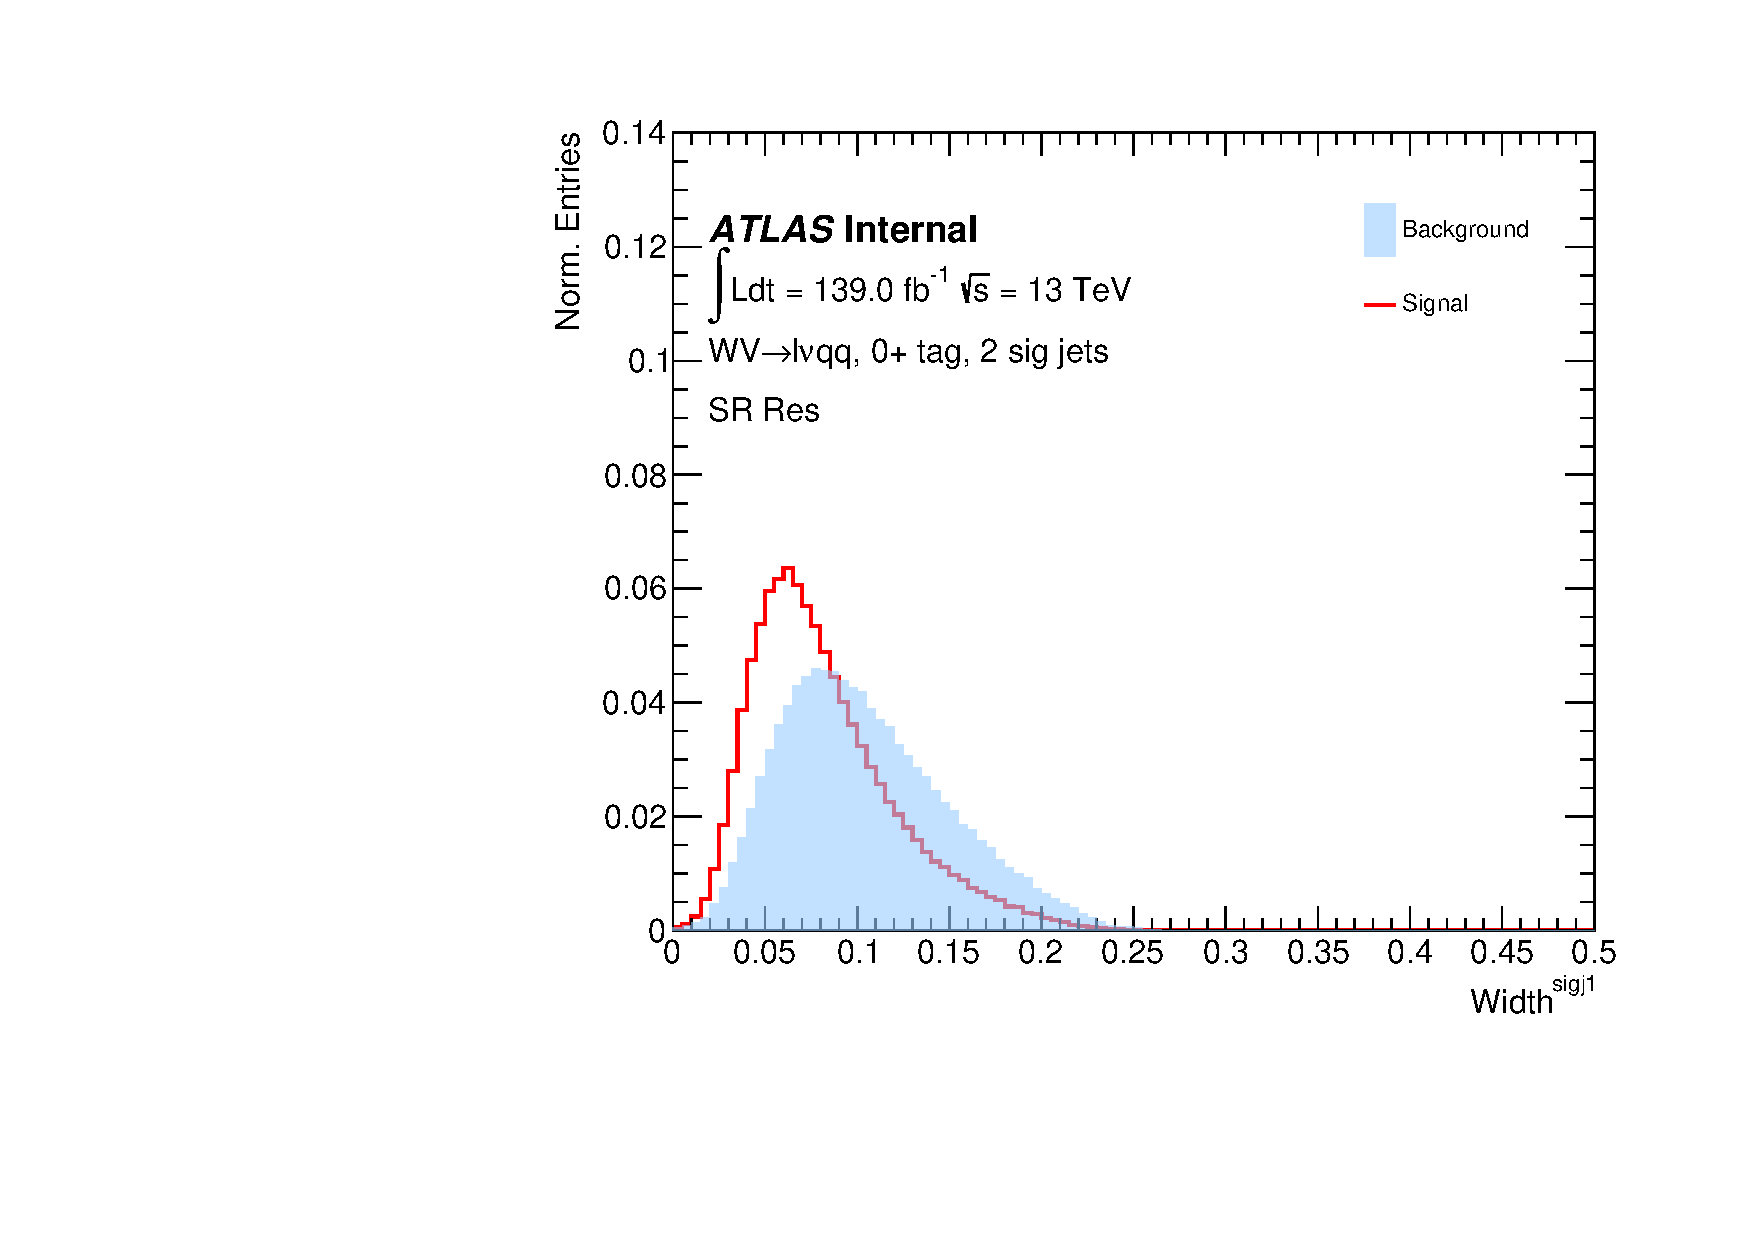
\includegraphics[width=0.3\textwidth]{figures/ml_dnn/variables/SR_Res/norm_plot_sigJ1_width.pdf}}\quad
  \subfloat[]{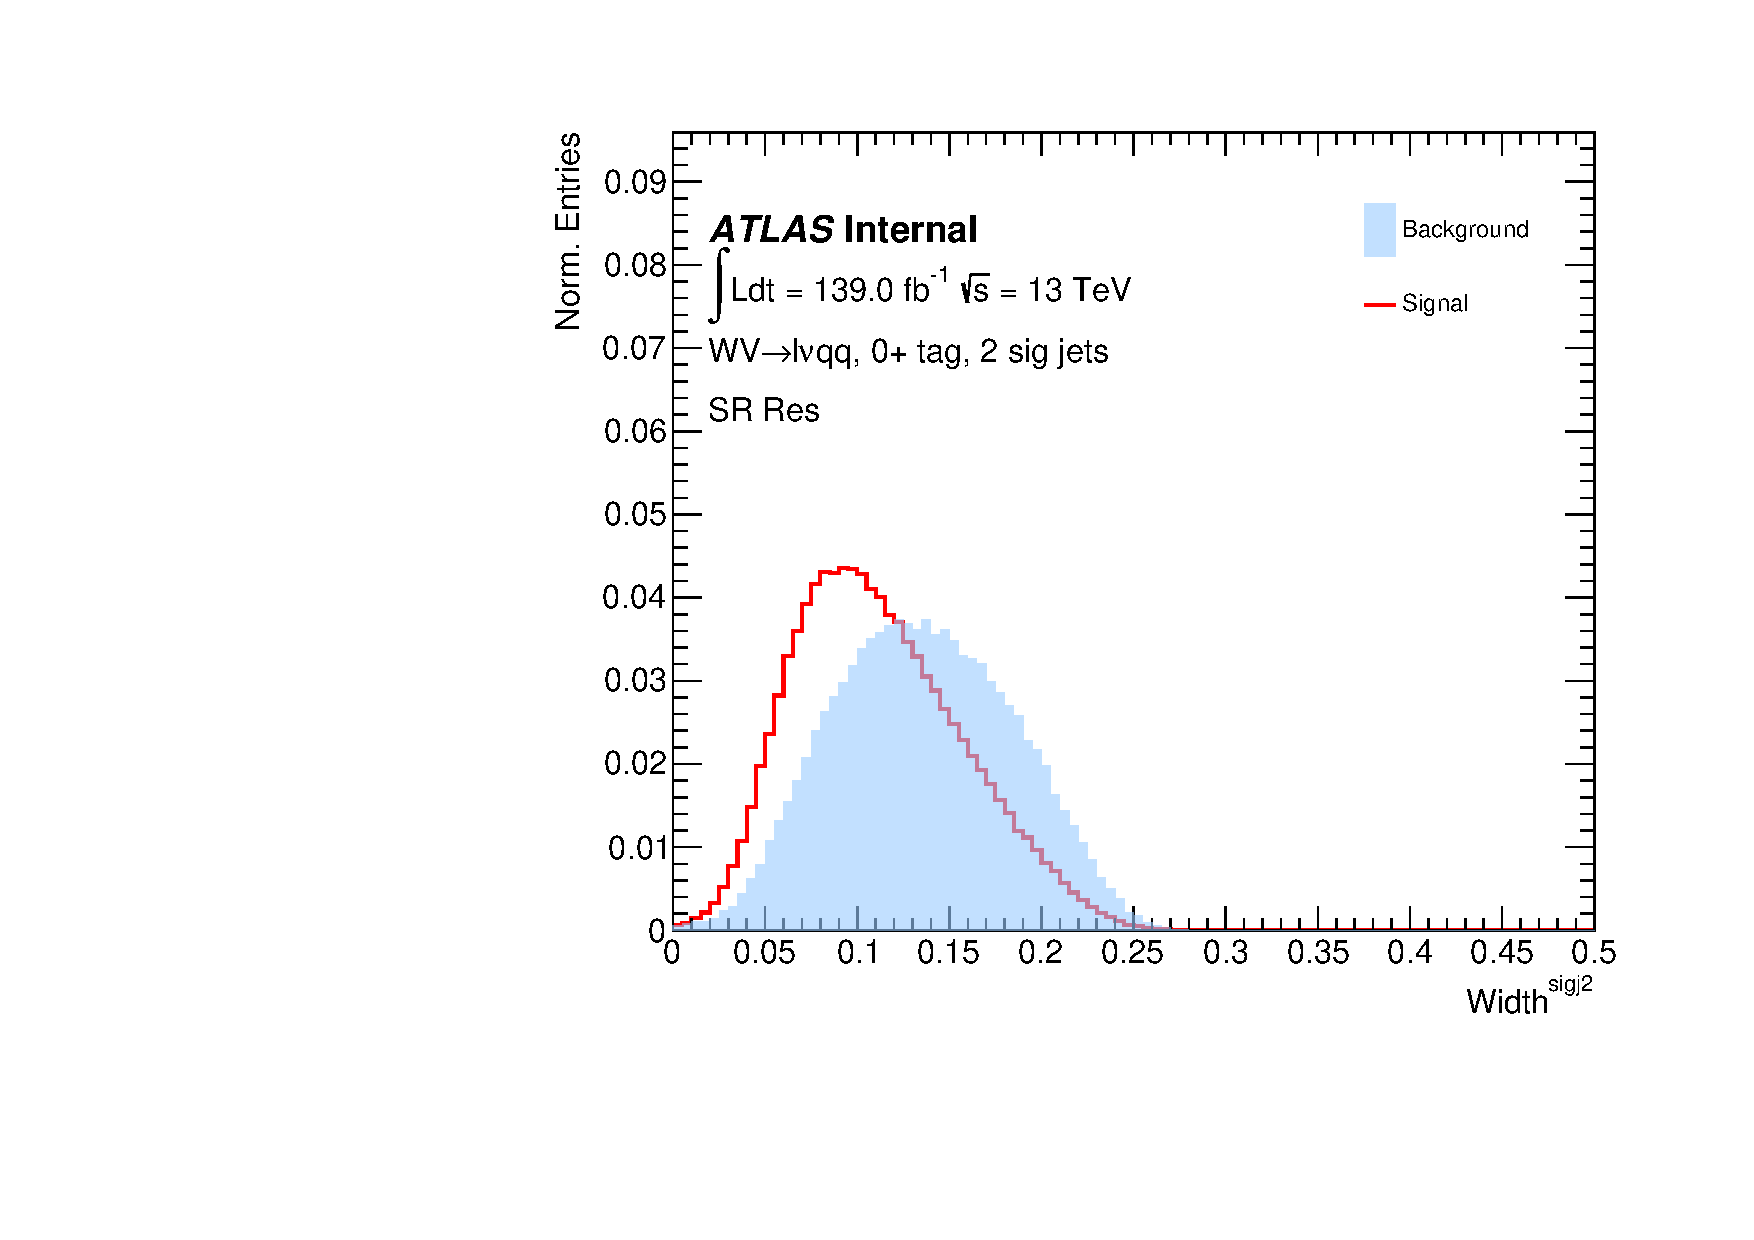
\includegraphics[width=0.3\textwidth]{figures/ml_dnn/variables/SR_Res/norm_plot_sigJ2_width.pdf}}\quad
  \subfloat[]{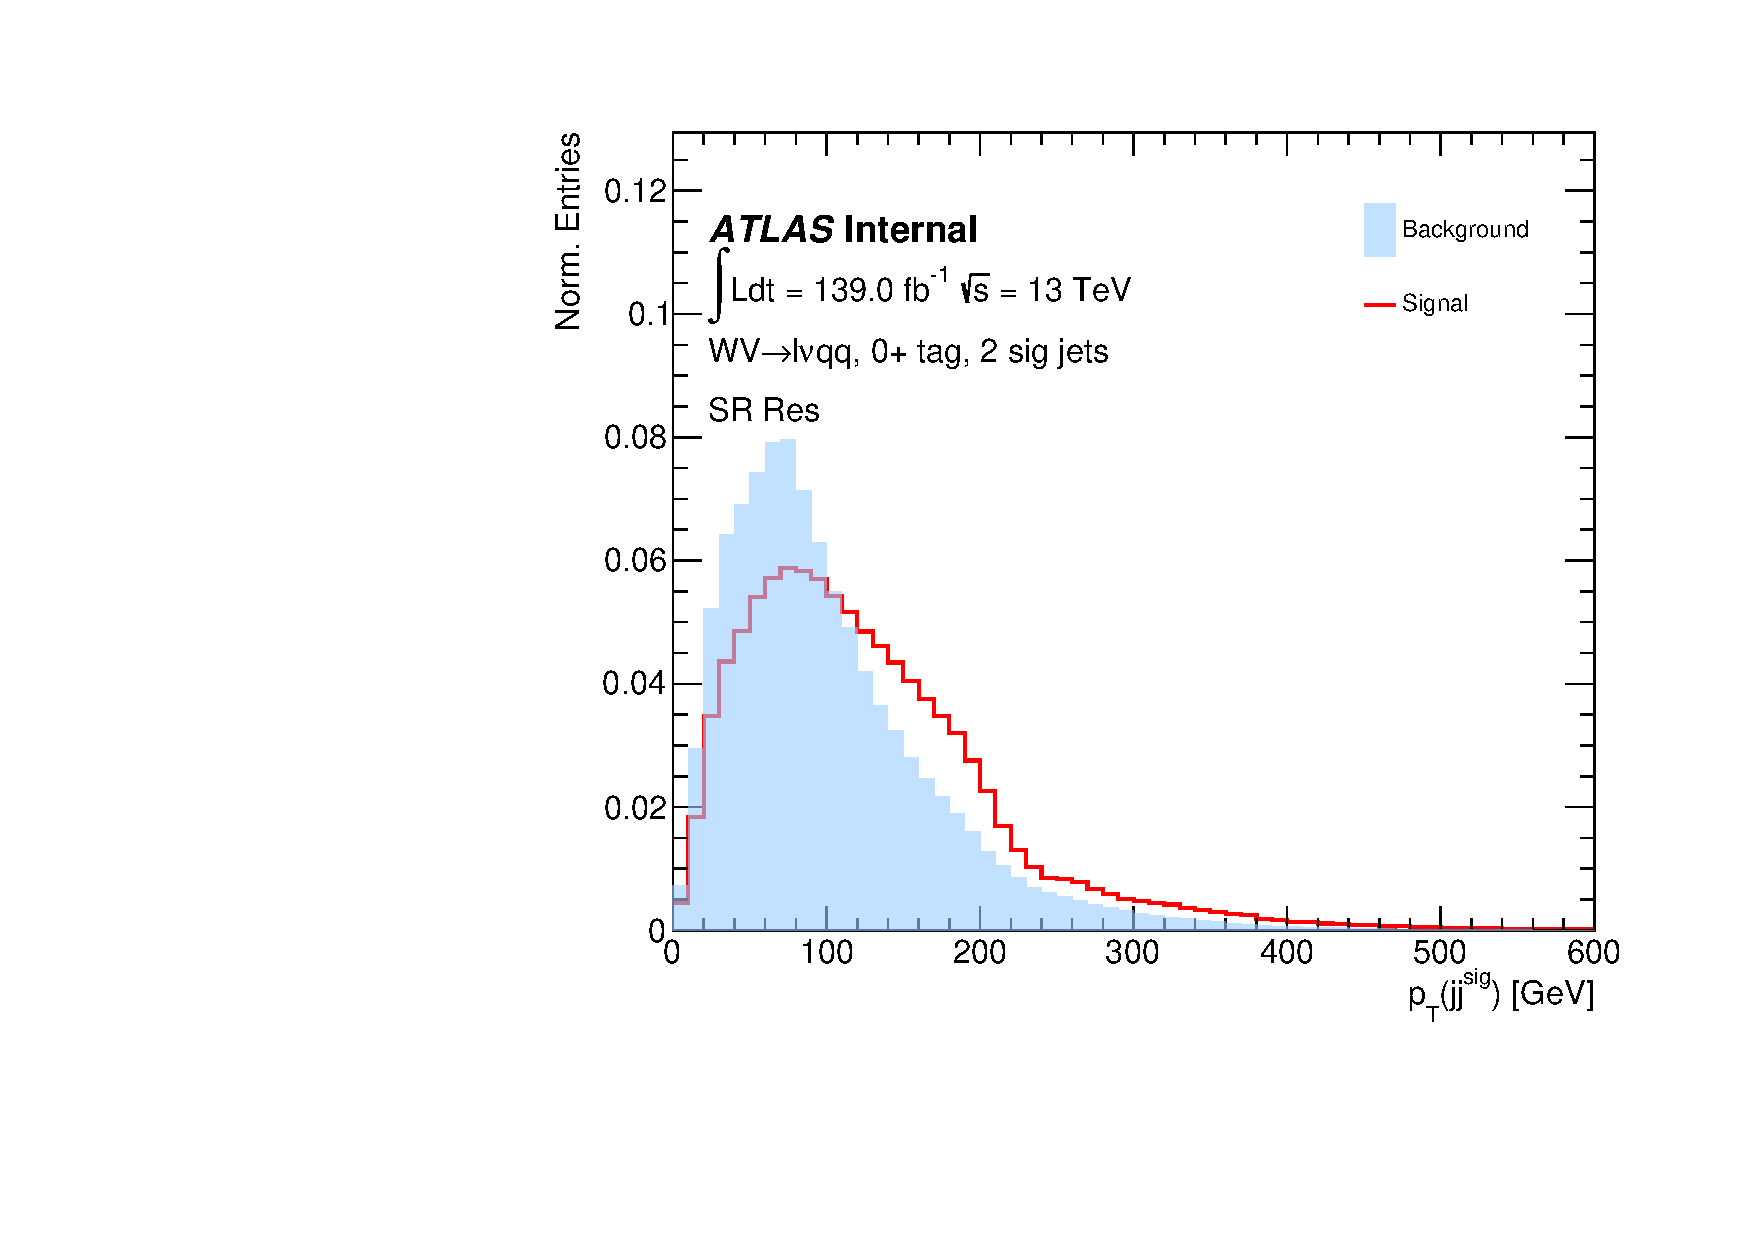
\includegraphics[width=0.3\textwidth]{figures/ml_dnn/variables/SR_Res/norm_plot_Dijet_pt.pdf}}
  
  % Row 3
  \subfloat[]{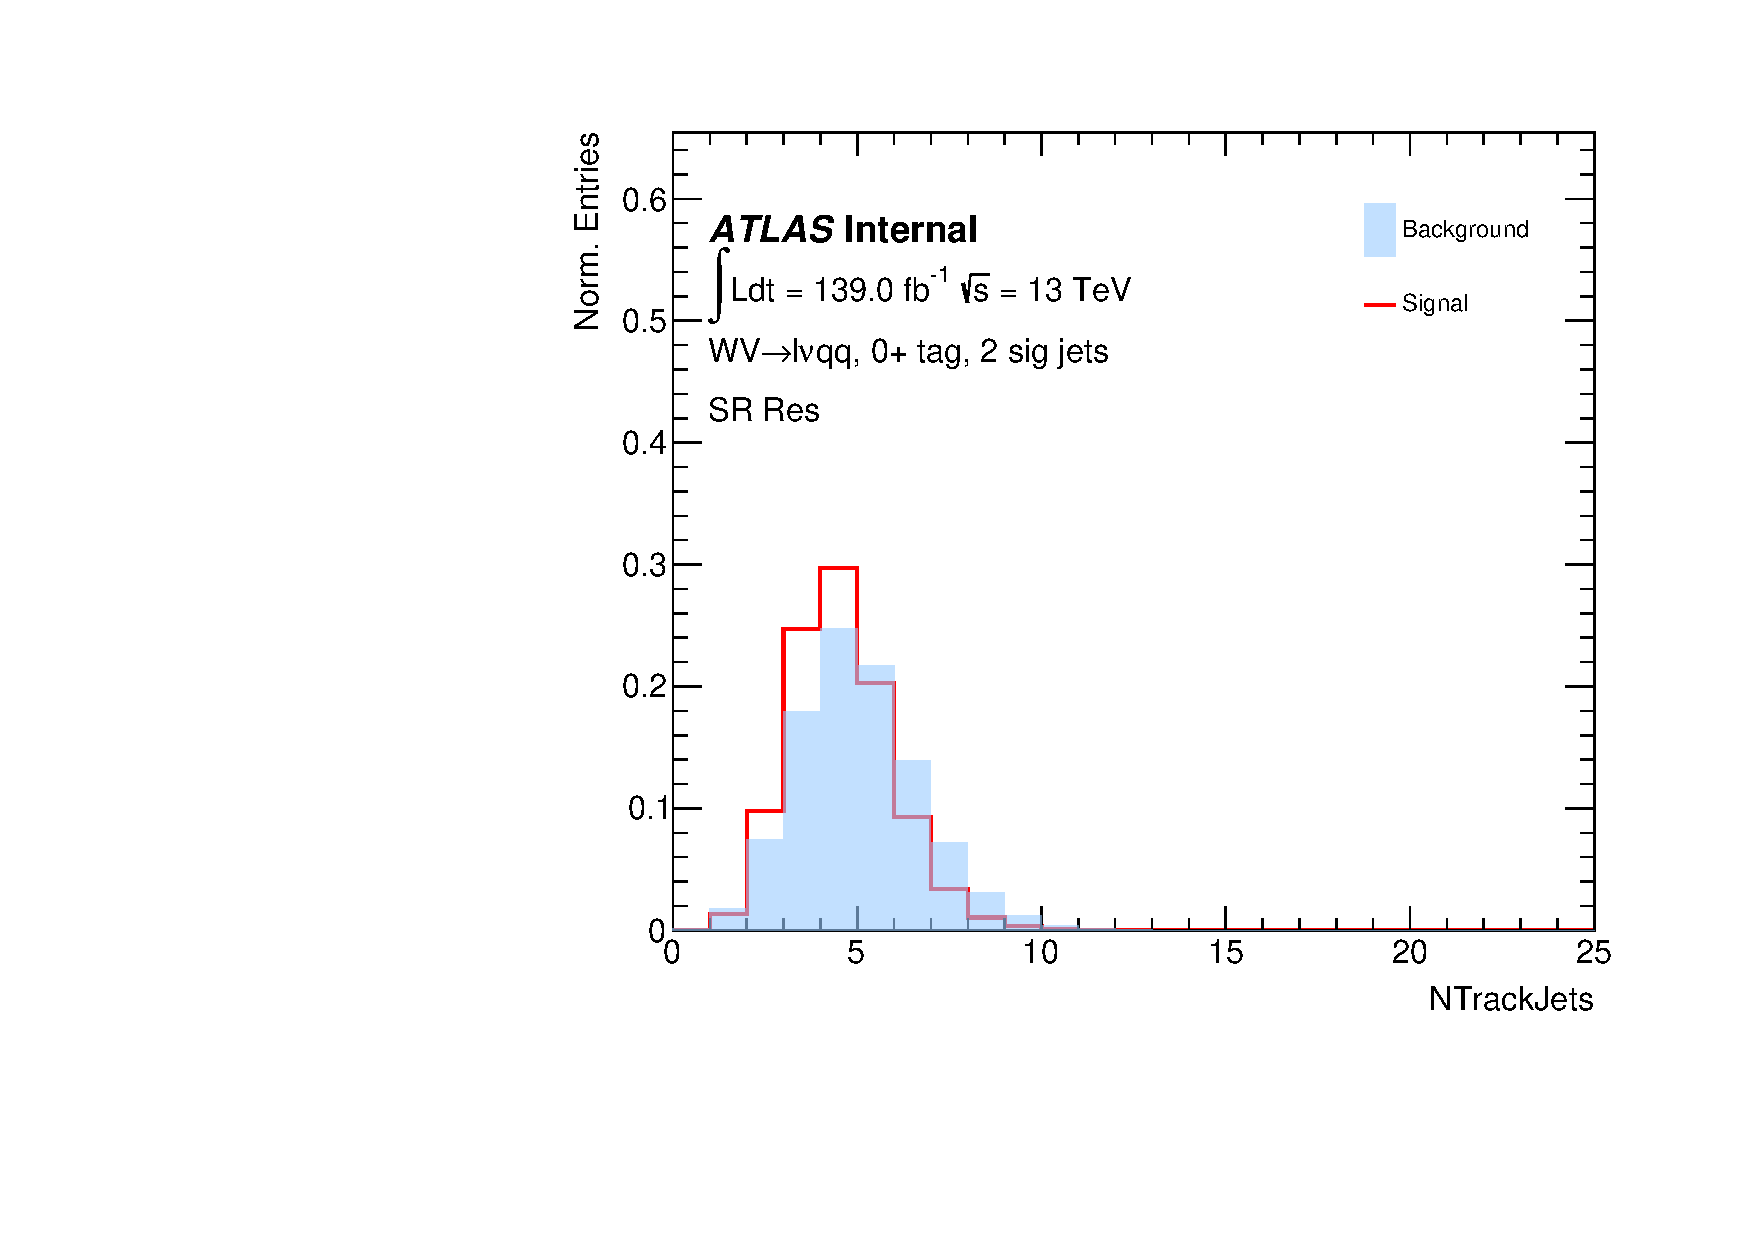
\includegraphics[width=0.3\textwidth]{figures/ml_dnn/variables/SR_Res/norm_plot_NTrackJets.pdf}}\quad
  \subfloat[]{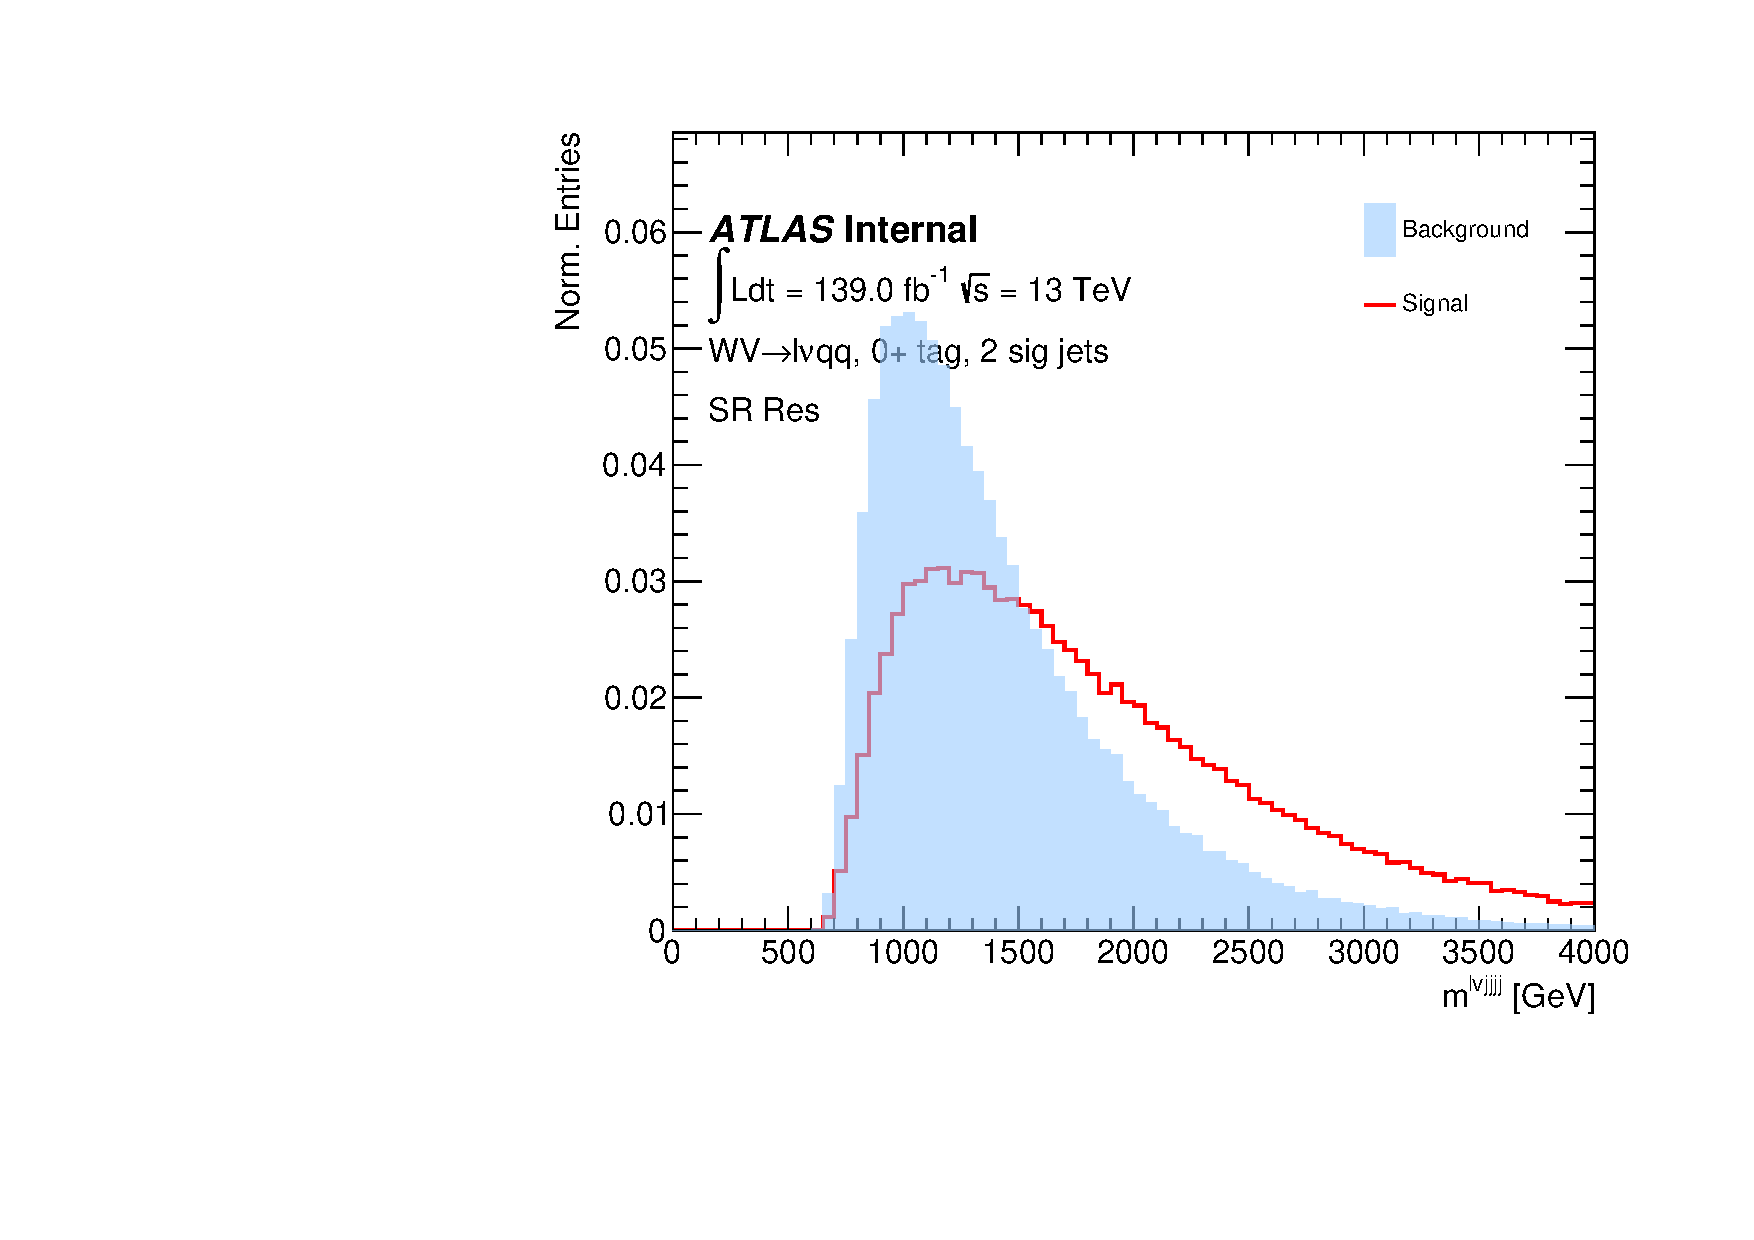
\includegraphics[width=0.3\textwidth]{figures/ml_dnn/variables/SR_Res/norm_plot_lvjjjjmass.pdf}}\quad
  \subfloat[]{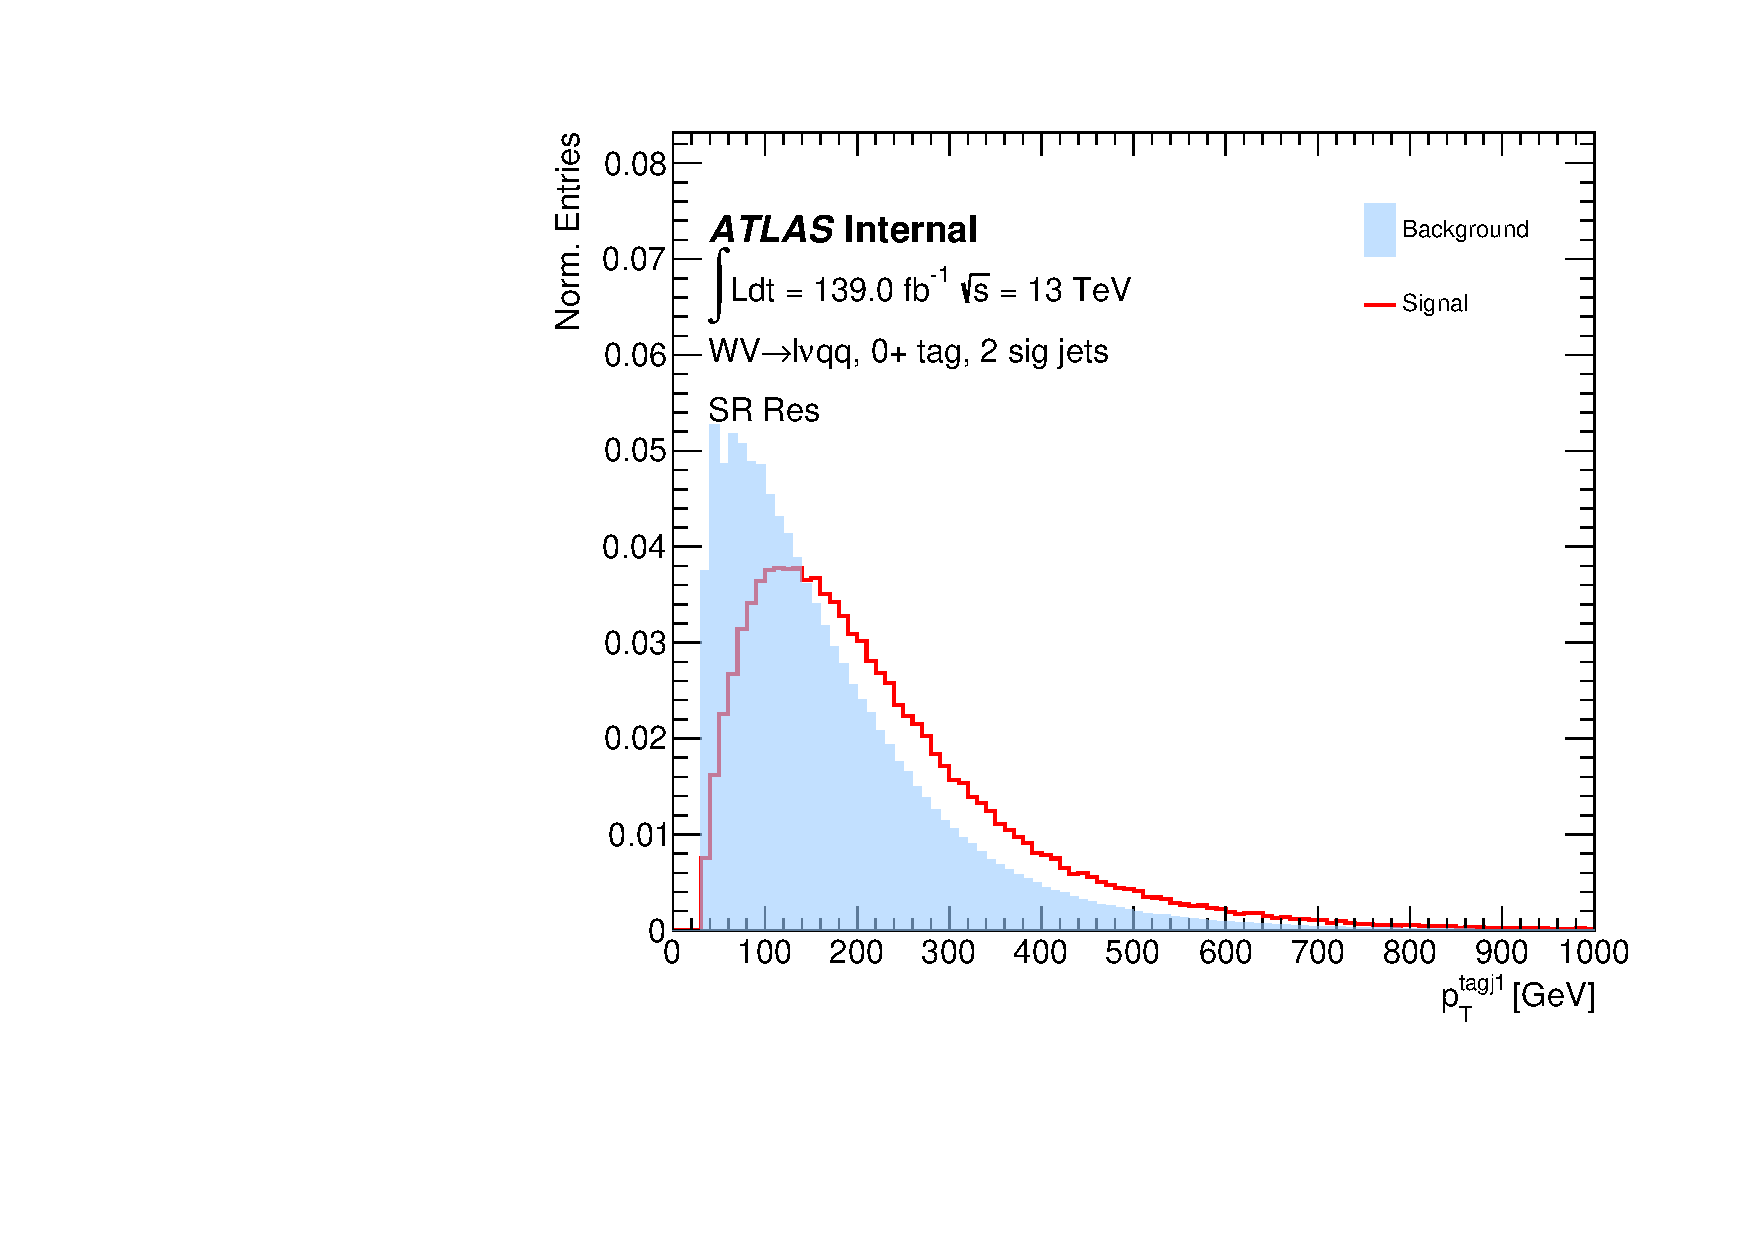
\includegraphics[width=0.3\textwidth]{figures/ml_dnn/variables/SR_Res/norm_plot_resolved_tagJ1_pt.pdf}}
  
 \caption{Distributions of input variables in the Resolved SR (Continued on next page)}
 \label{fig:res_inputs-part1}
\end{figure}

\begin{figure}[ht]
 \centering

  % Row 4
  \subfloat[]{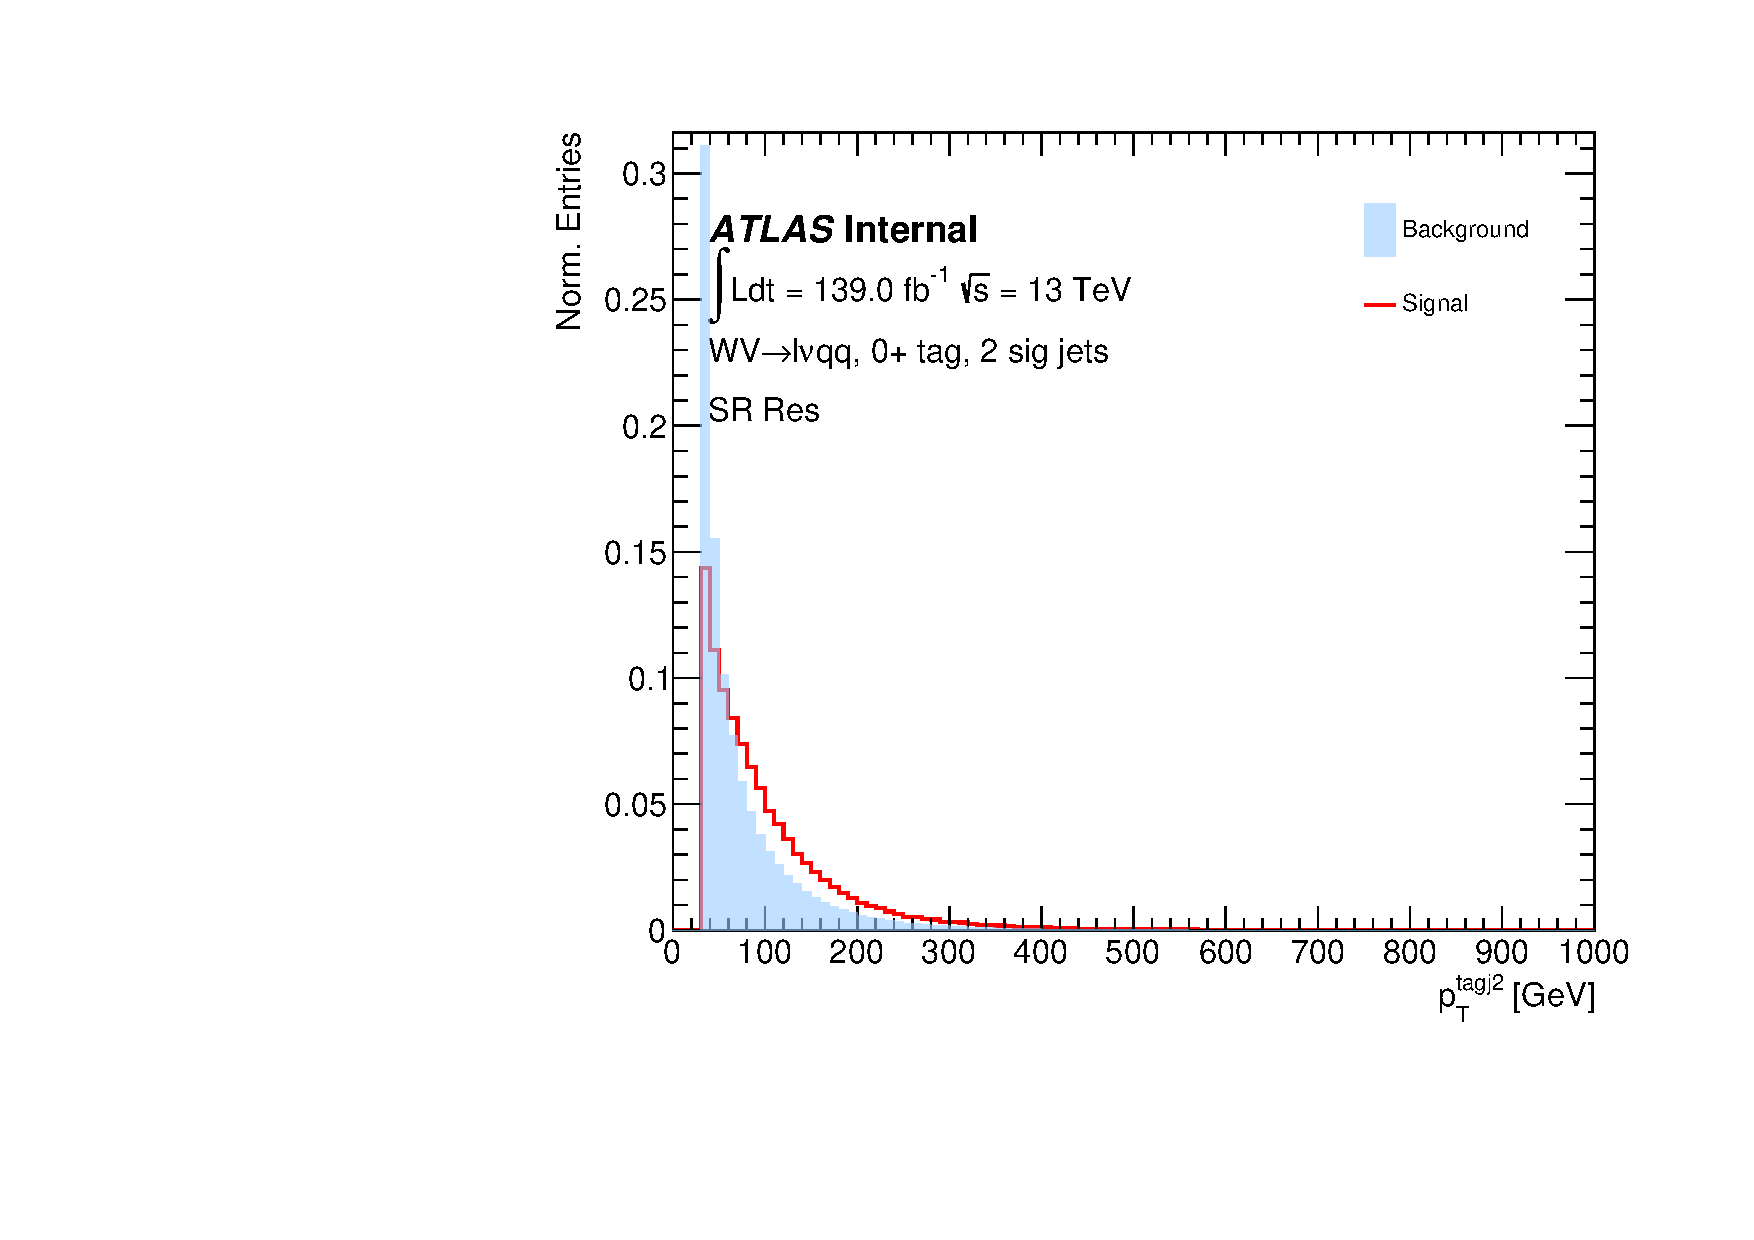
\includegraphics[width=0.3\textwidth]{figures/ml_dnn/variables/SR_Res/norm_plot_resolved_tagJ2_pt.pdf}}\quad
  \subfloat[]{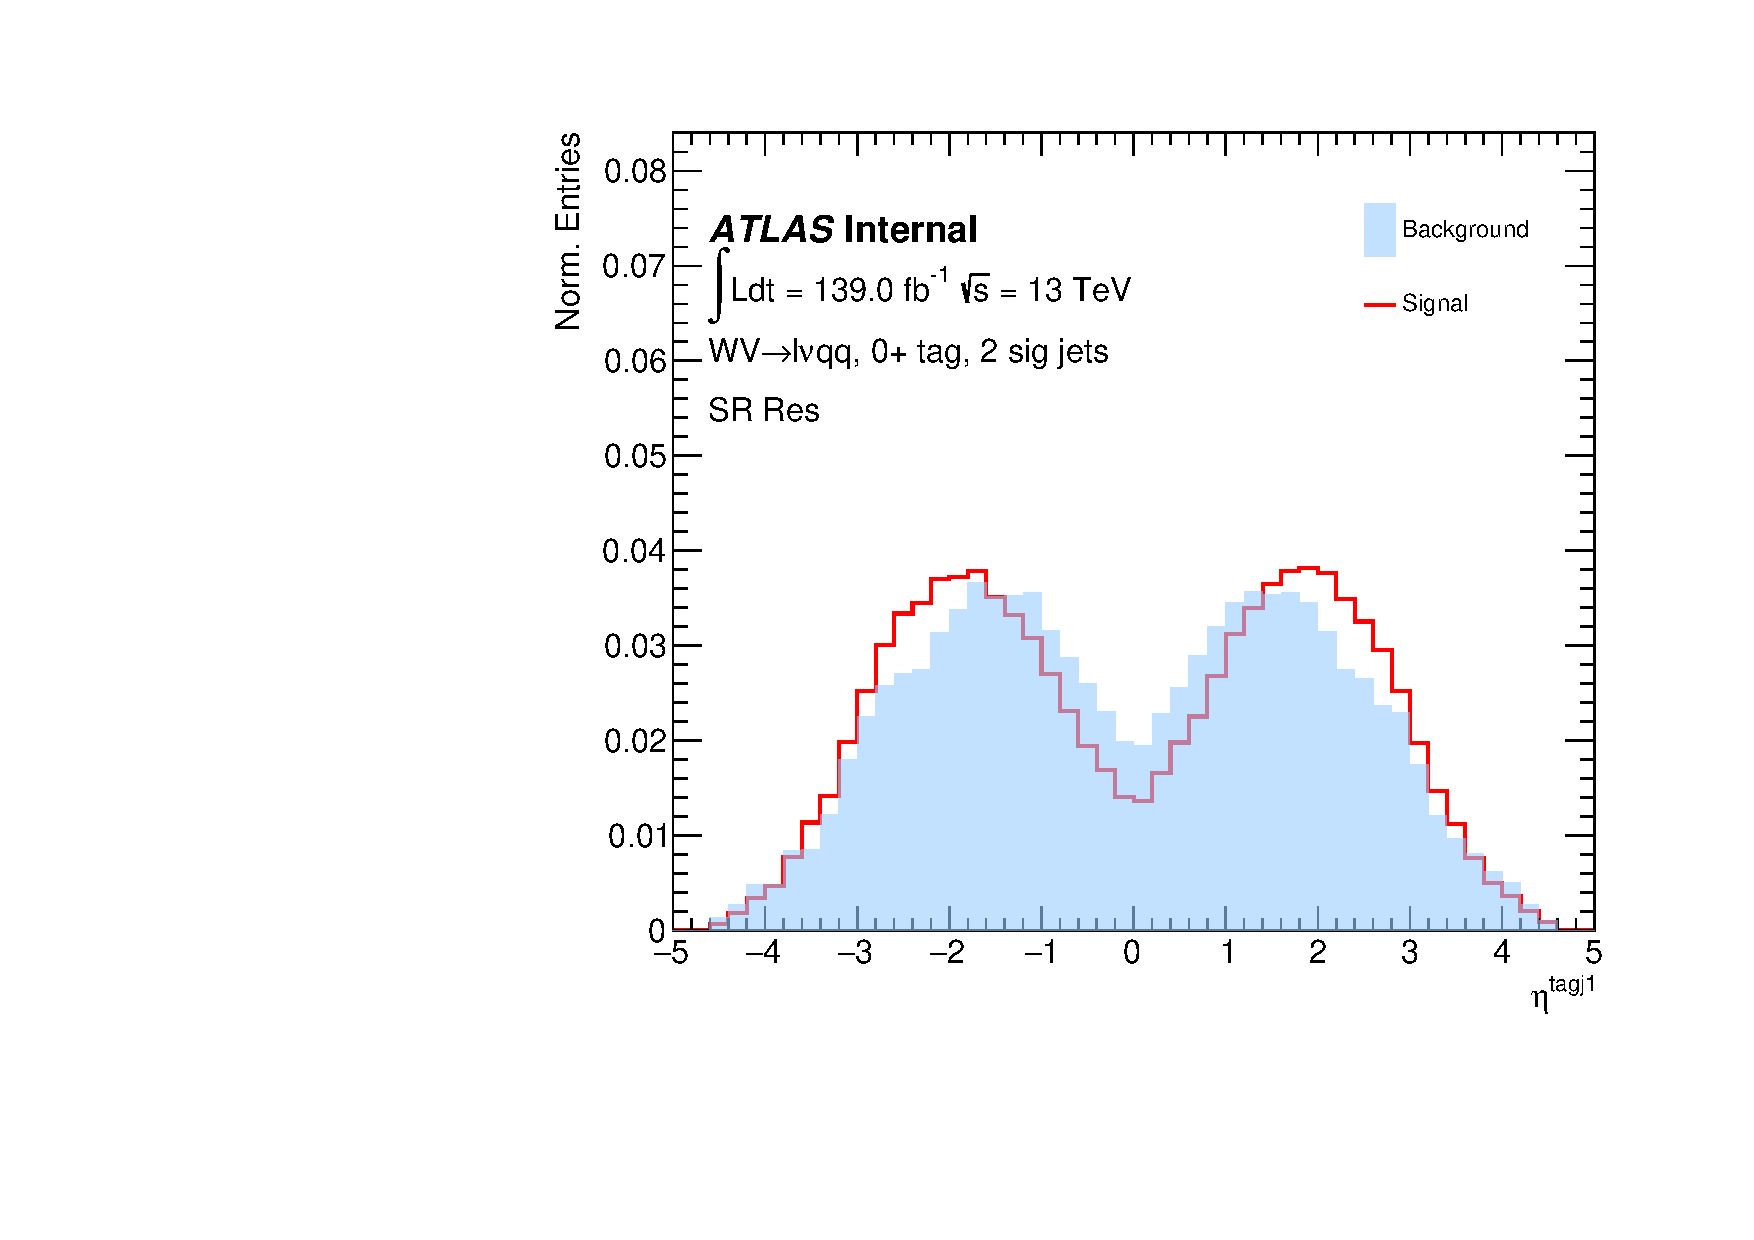
\includegraphics[width=0.3\textwidth]{figures/ml_dnn/variables/SR_Res/norm_plot_resolved_tagJ1_eta.pdf}}\quad
  \subfloat[]{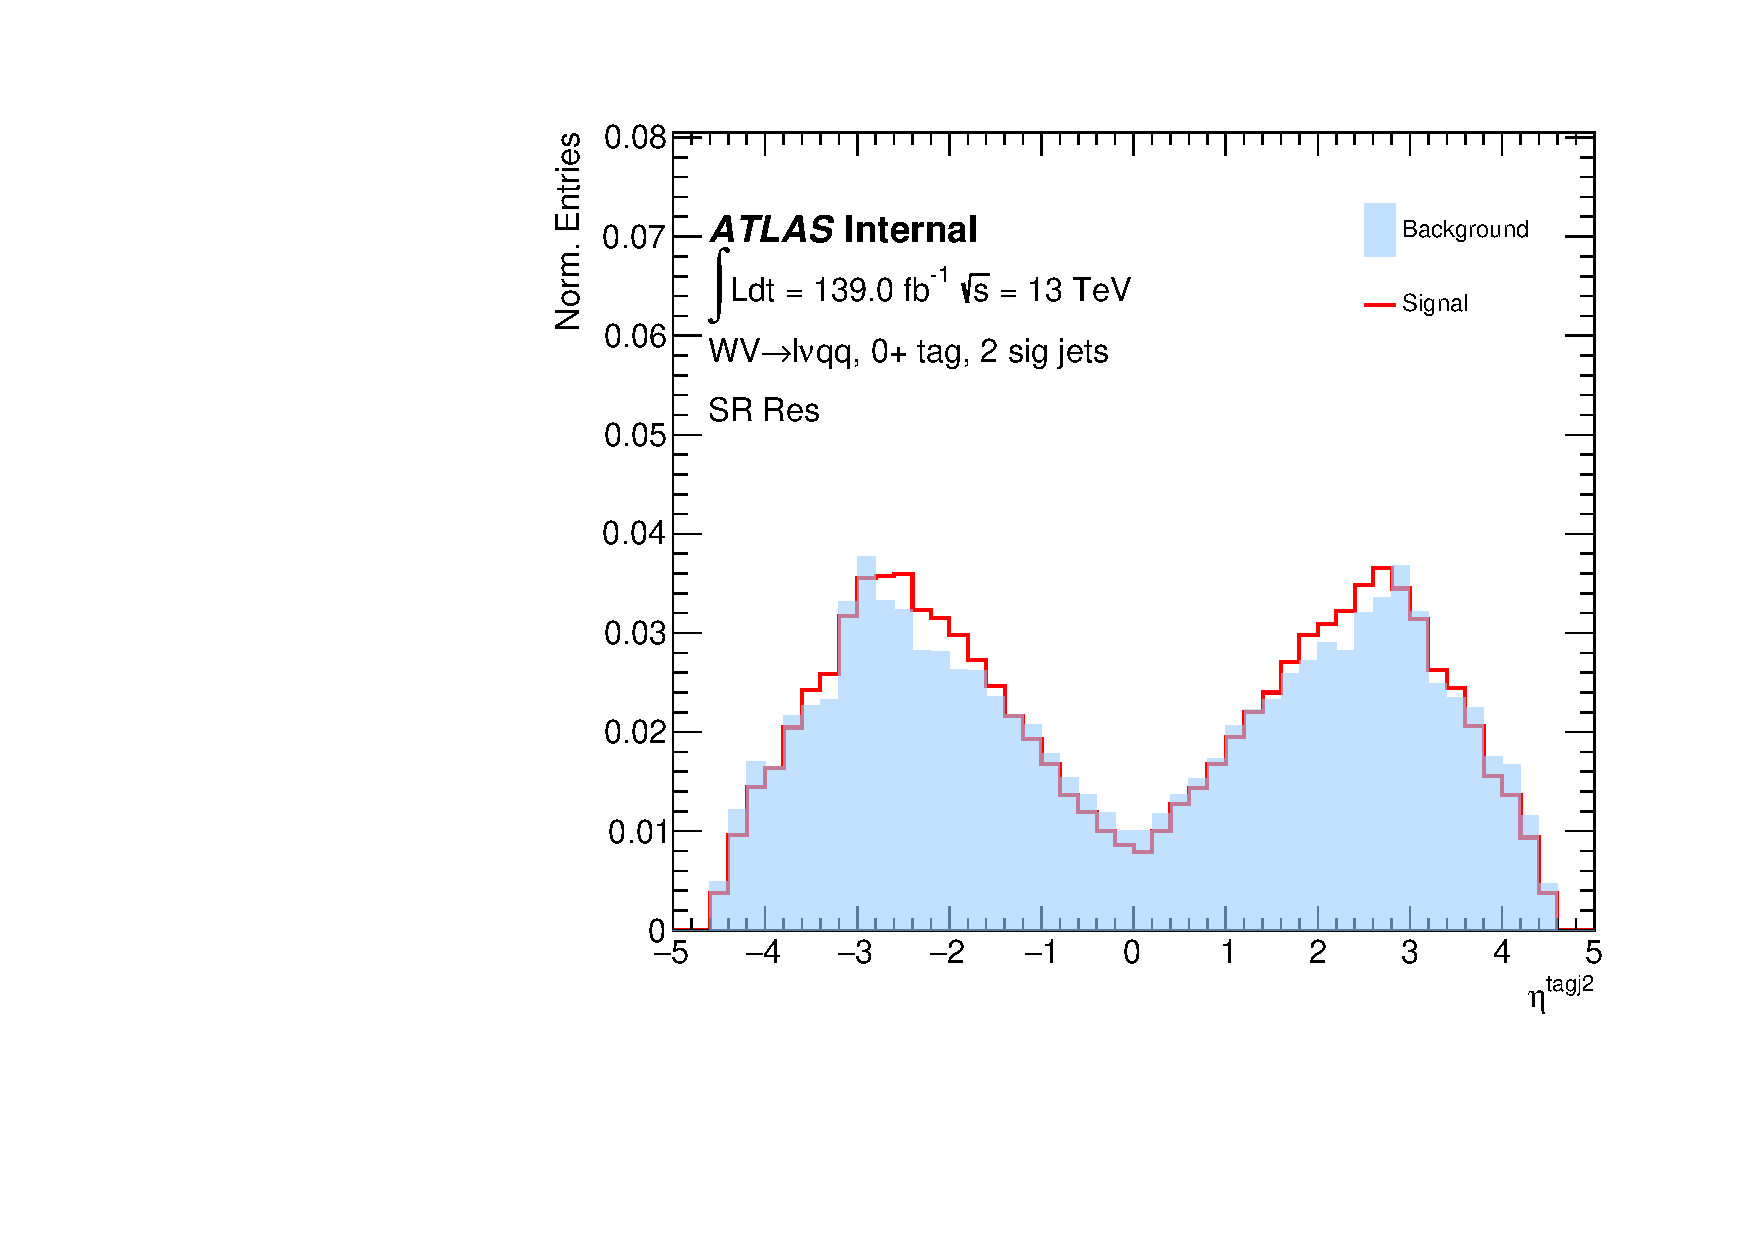
\includegraphics[width=0.3\textwidth]{figures/ml_dnn/variables/SR_Res/norm_plot_resolved_tagJ2_eta.pdf}}
  
  % Row 5
  \subfloat[]{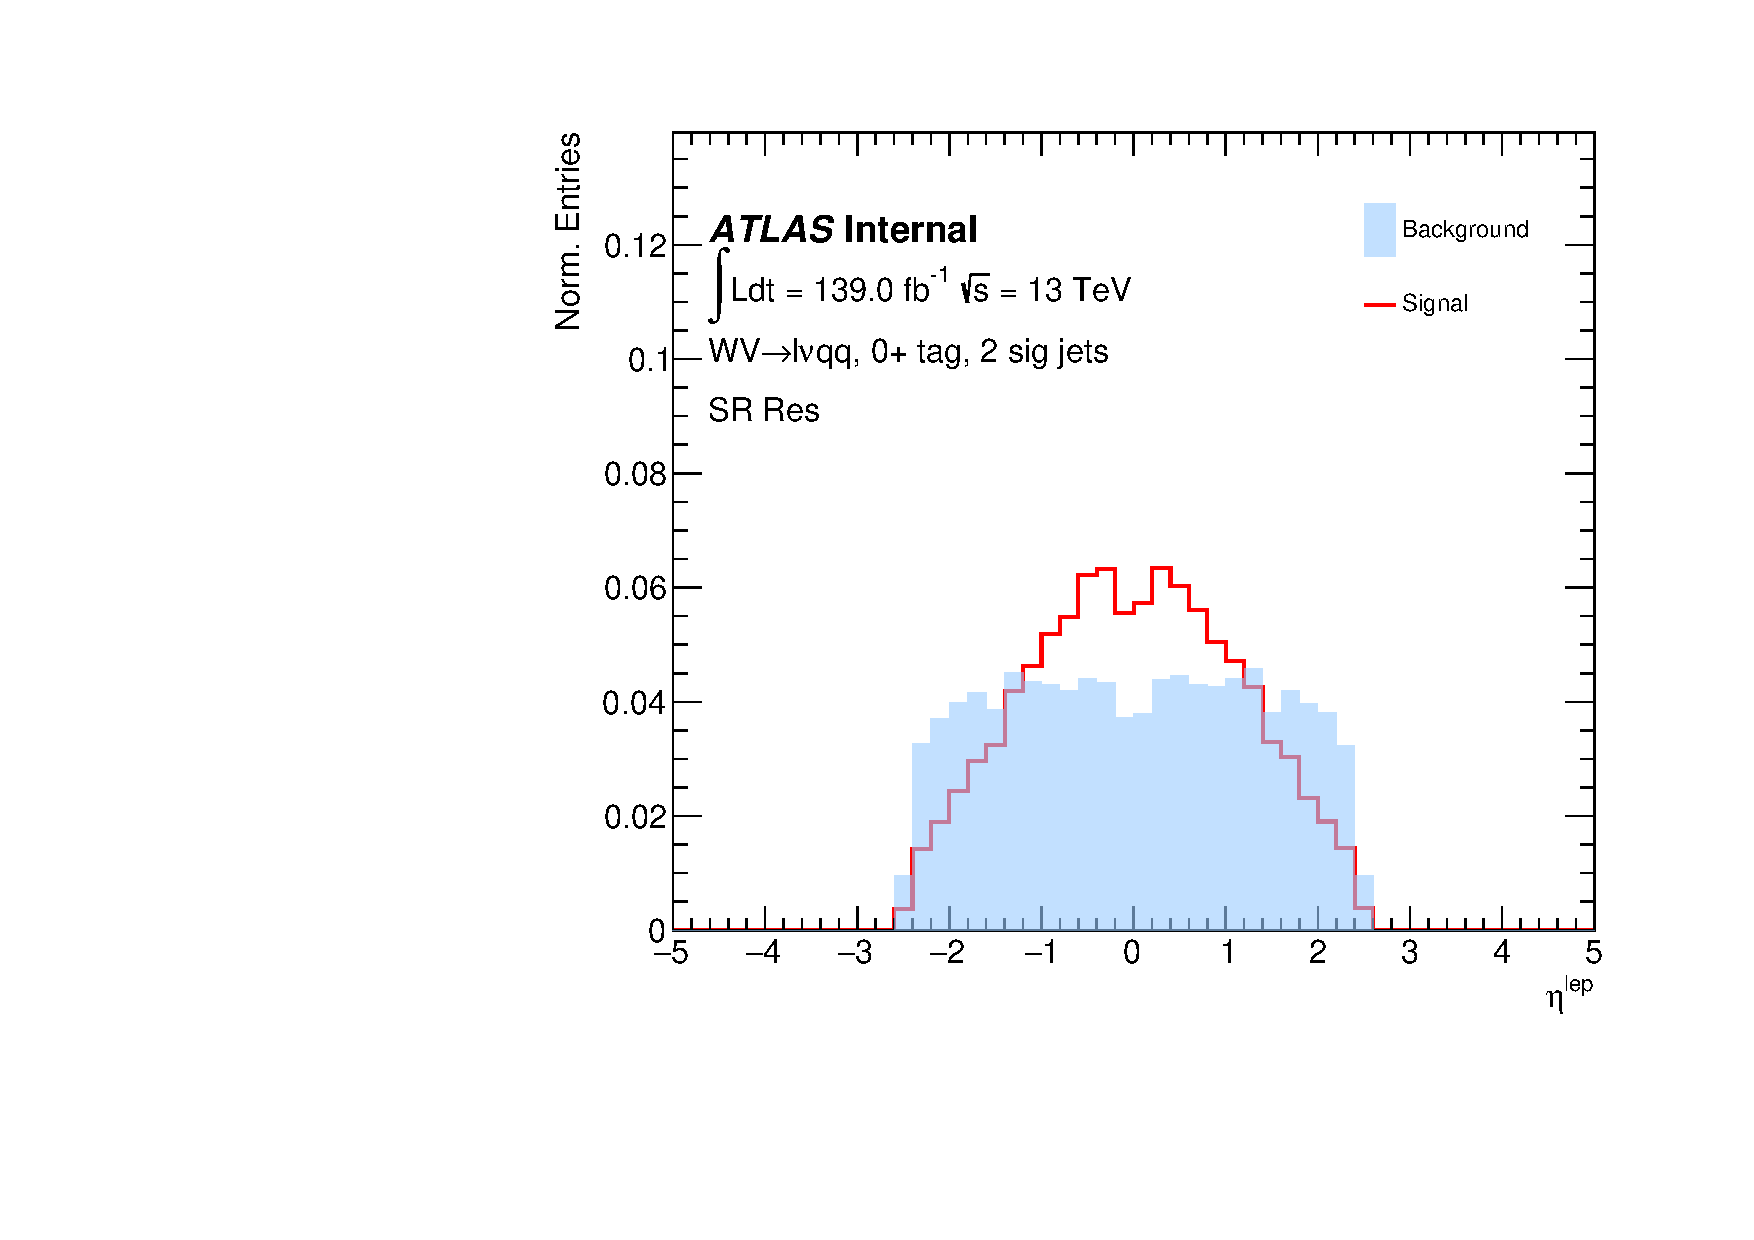
\includegraphics[width=0.3\textwidth]{figures/ml_dnn/variables/SR_Res/norm_plot_lep_eta.pdf}}\quad
  \subfloat[]{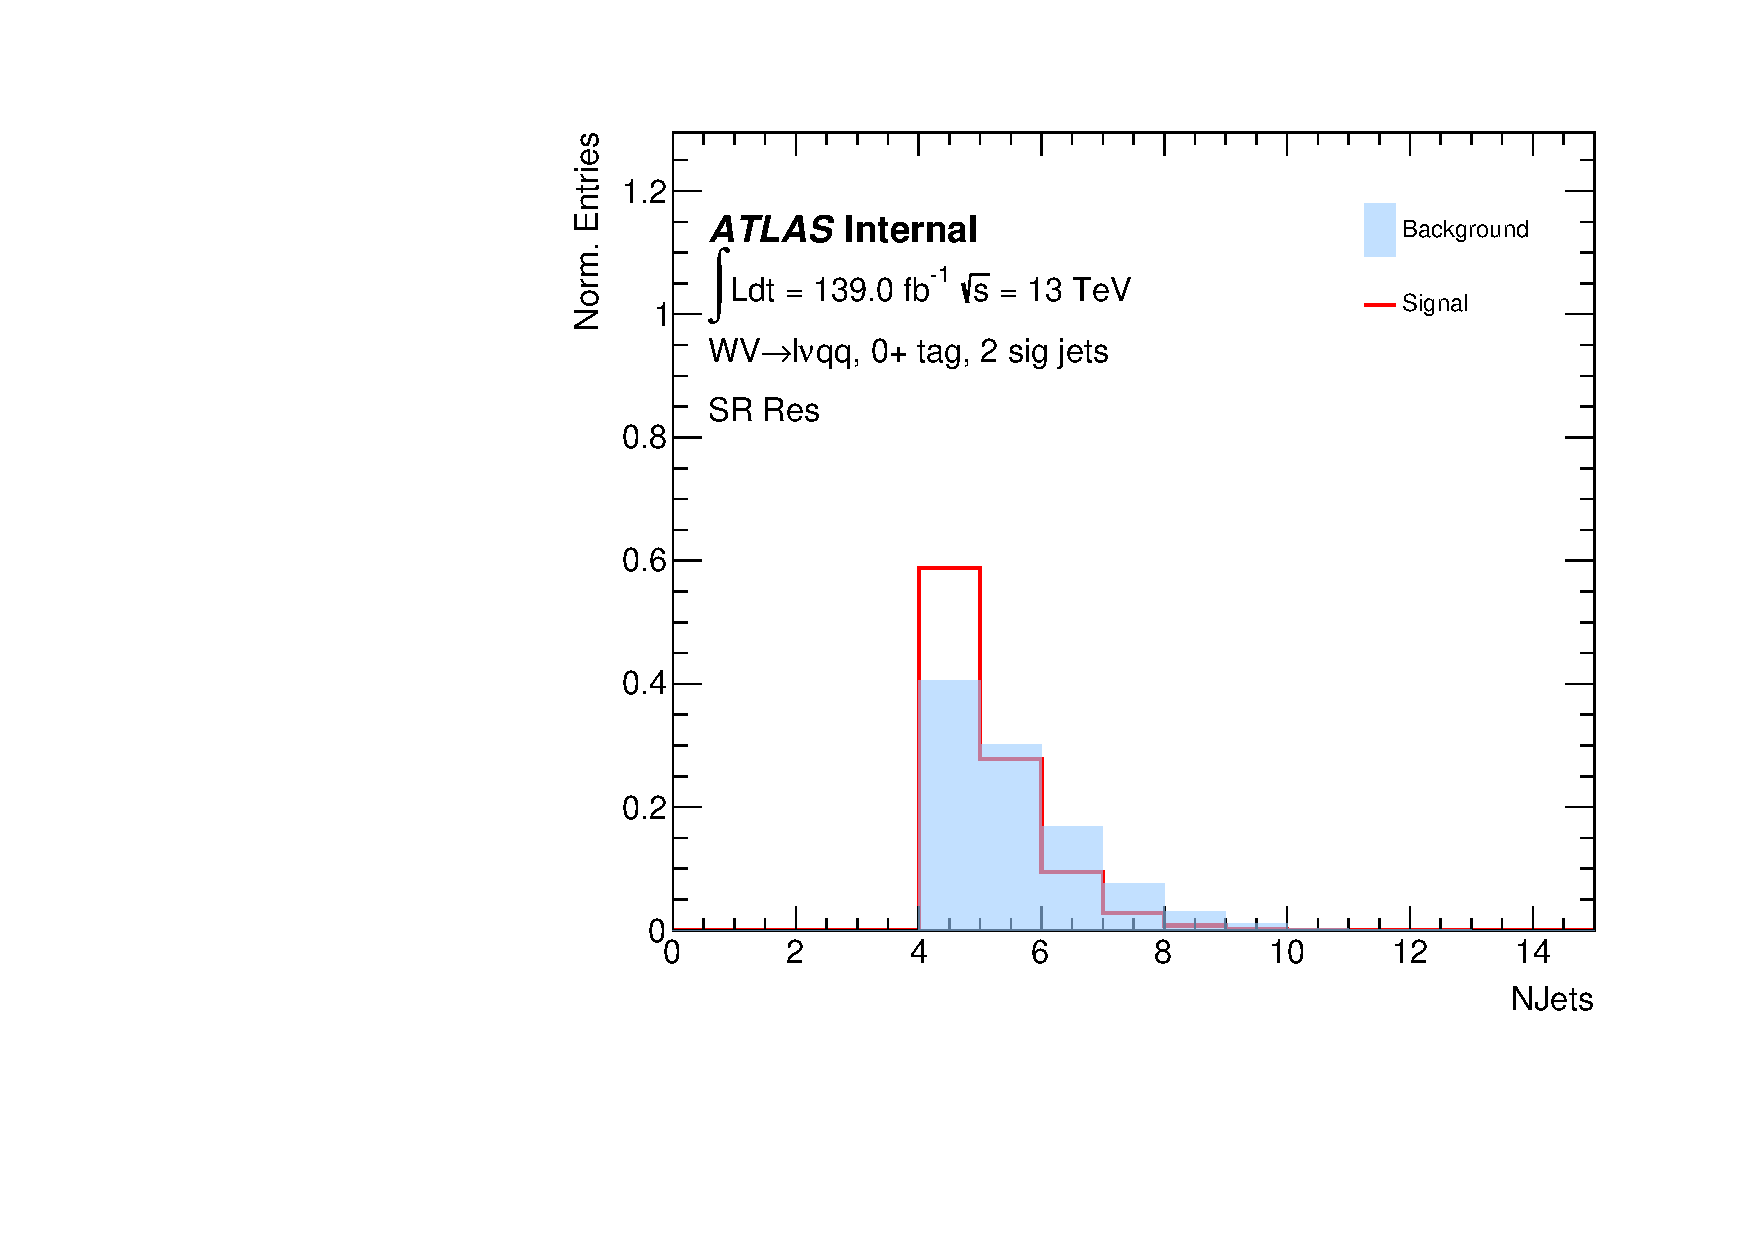
\includegraphics[width=0.3\textwidth]{figures/ml_dnn/variables/SR_Res/norm_plot_NJets.pdf}}\quad
  \subfloat[]{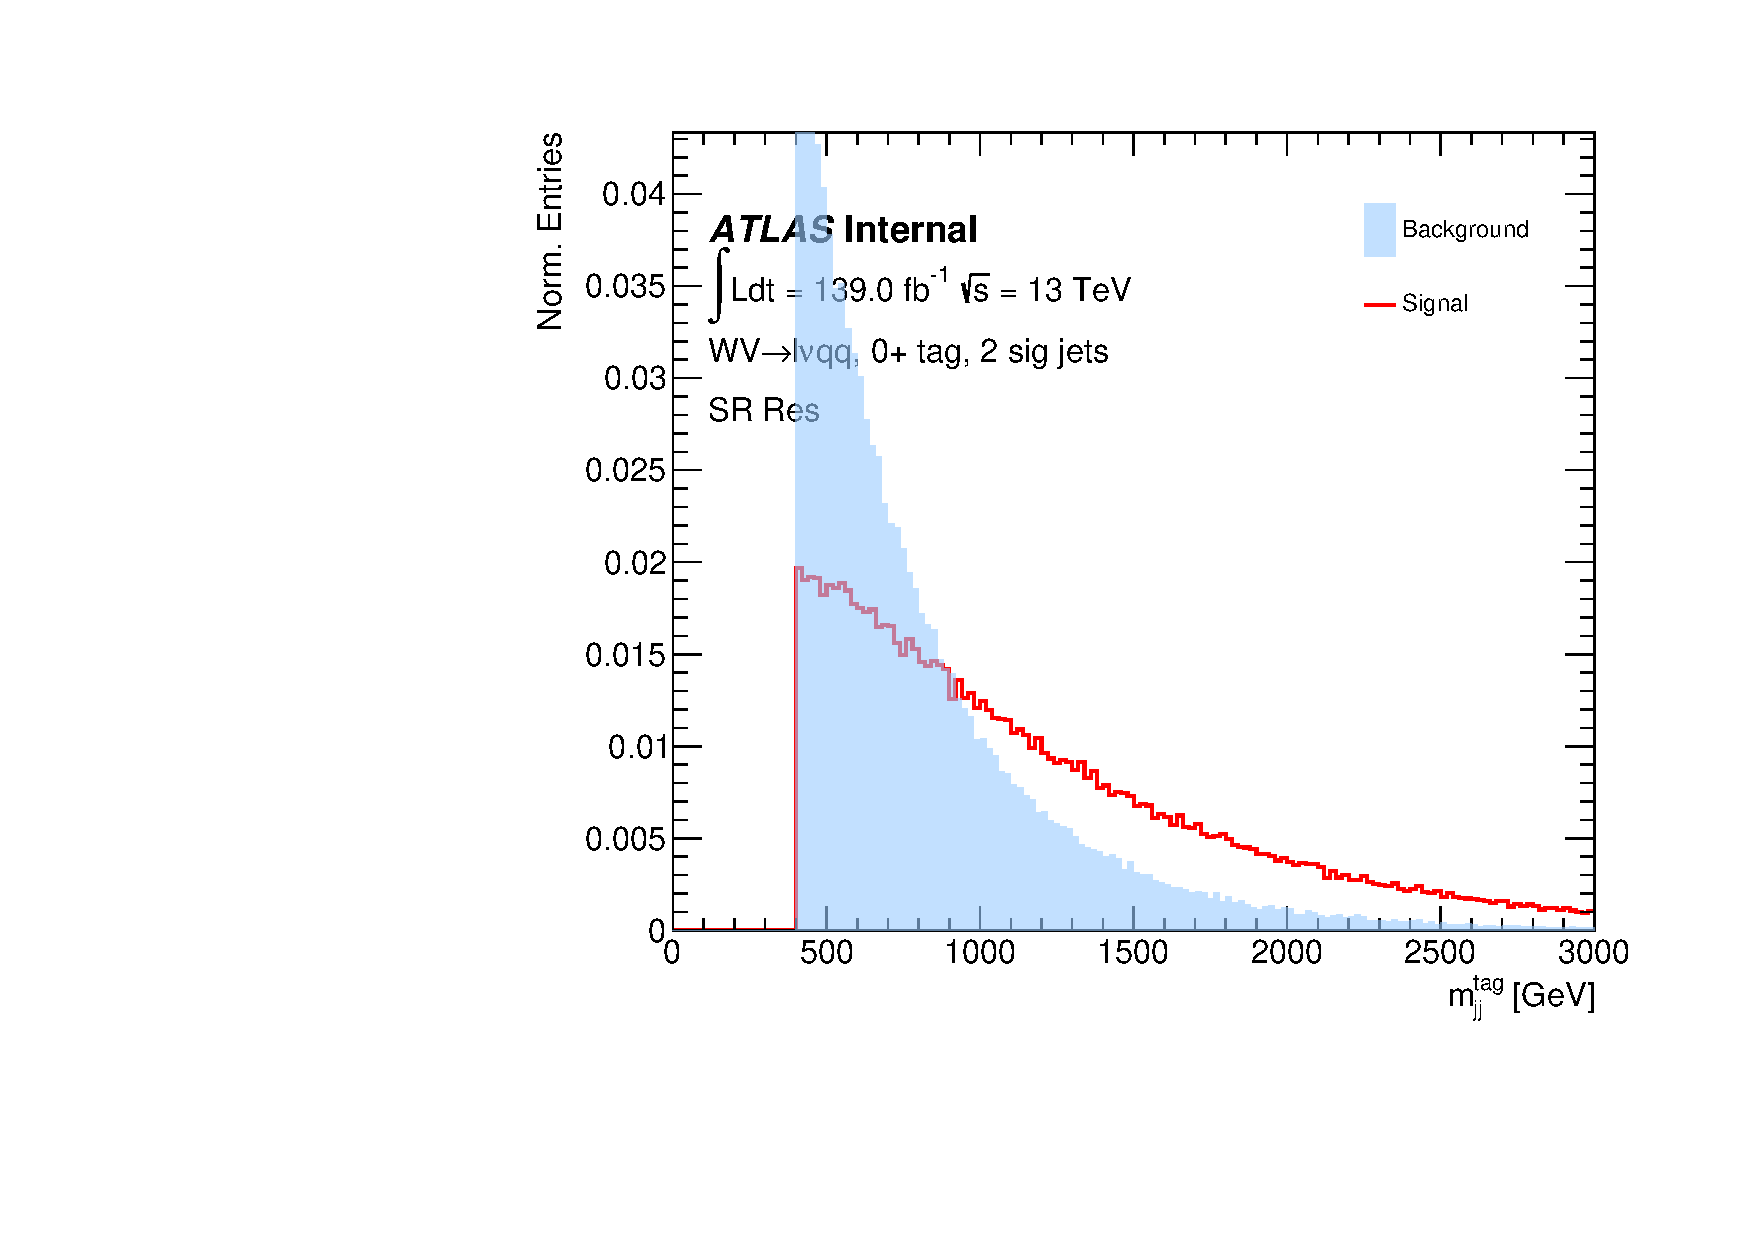
\includegraphics[width=0.3\textwidth]{figures/ml_dnn/variables/SR_Res/norm_plot_resolved_tagMjj.pdf}}
  
  % Row 6
  \subfloat[]{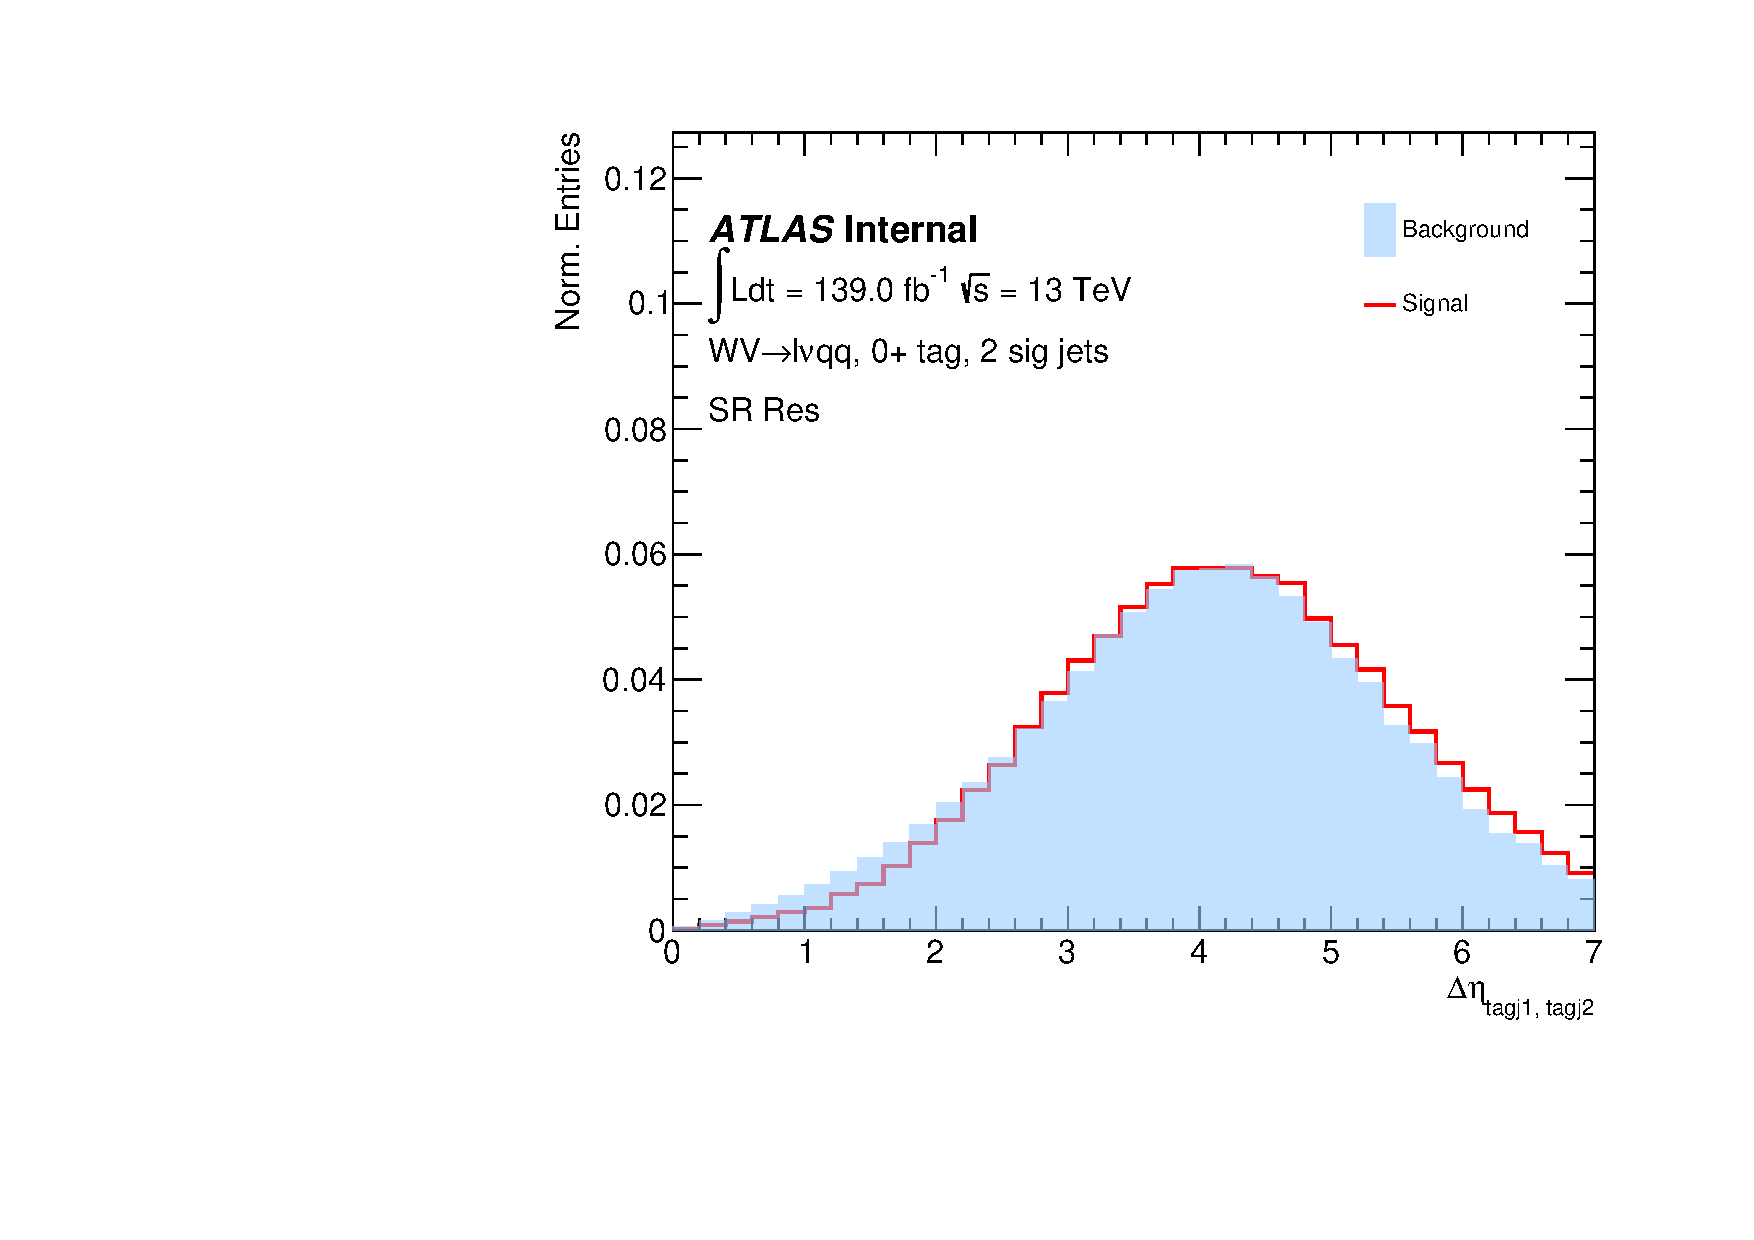
\includegraphics[width=0.3\textwidth]{figures/ml_dnn/variables/SR_Res/norm_plot_resolved_tagJdEta.pdf}}\quad
  \subfloat[]{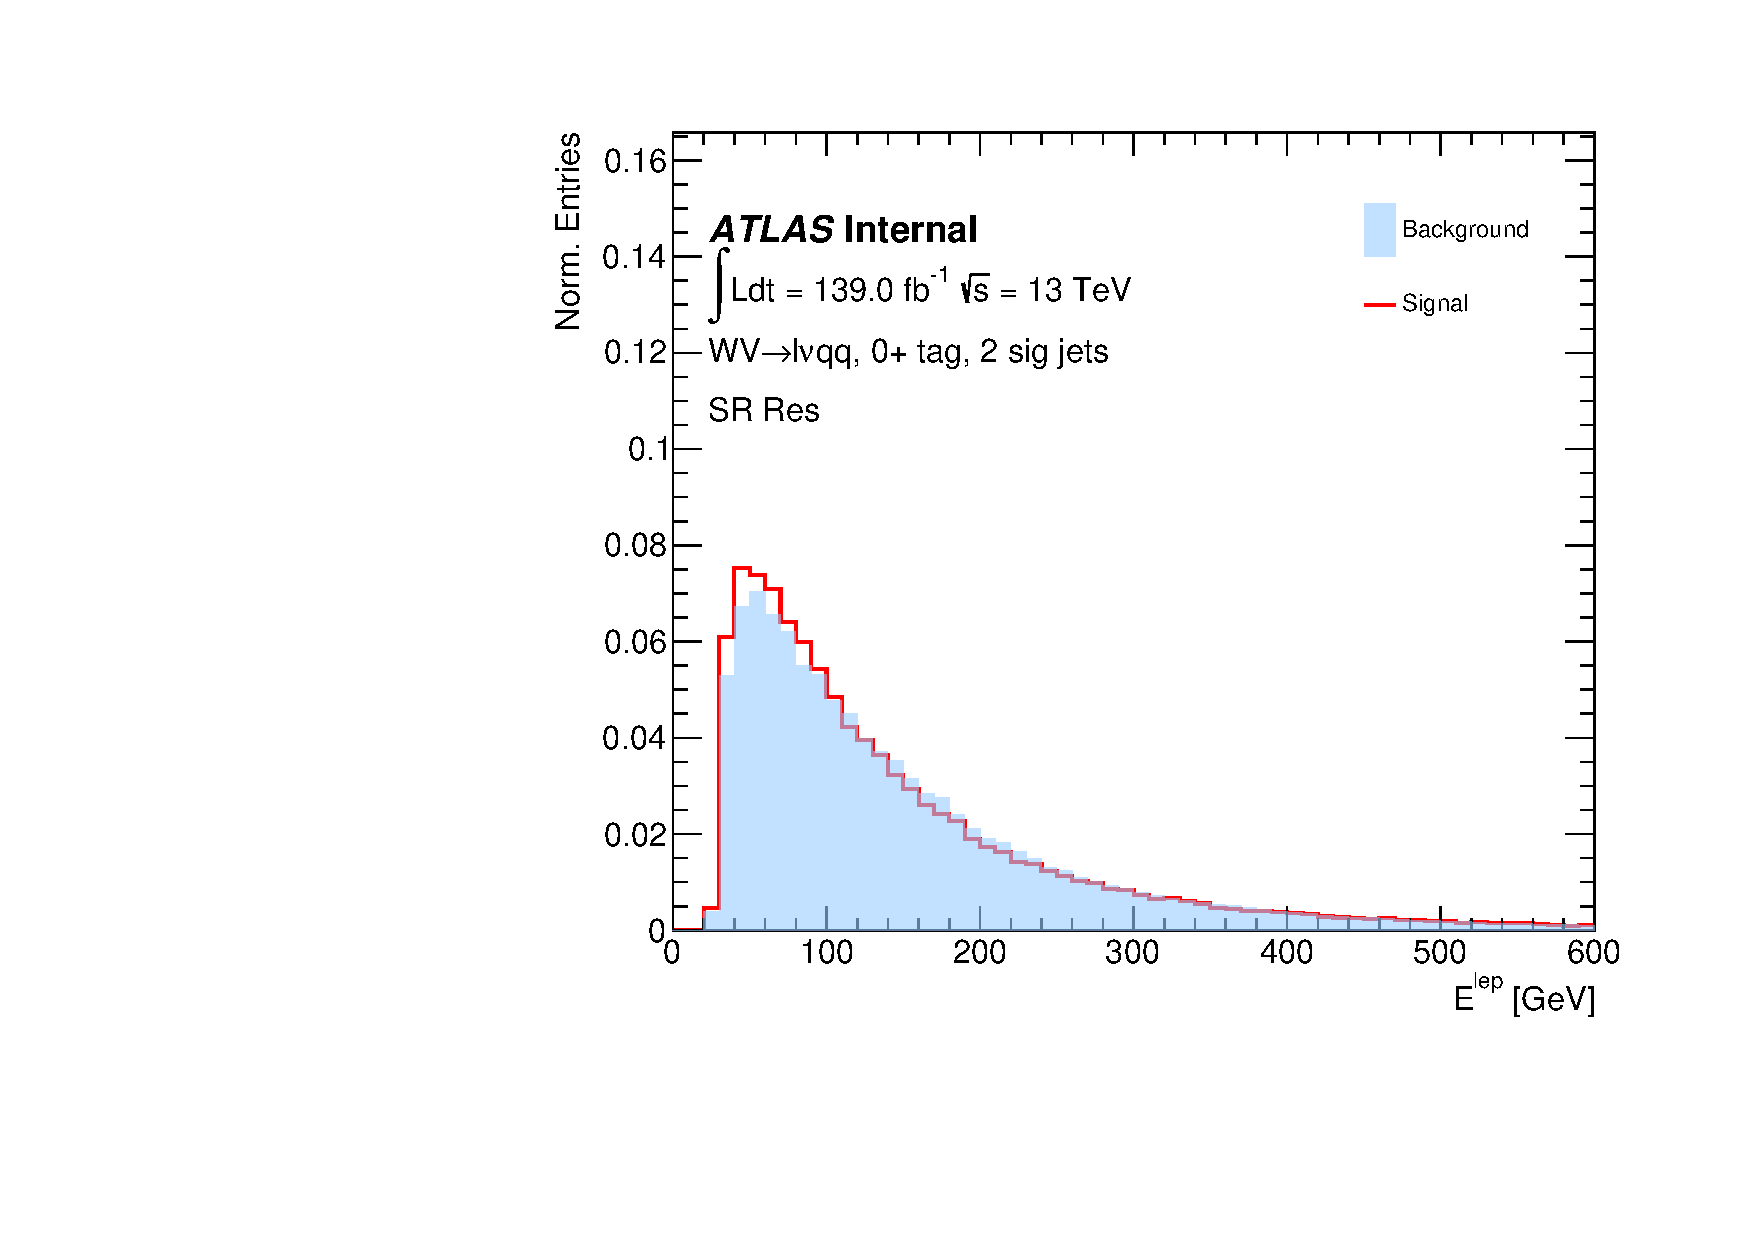
\includegraphics[width=0.3\textwidth]{figures/ml_dnn/variables/SR_Res/norm_plot_lep_e.pdf}}
  
  \caption{Distributions of input variables in the Resolved SR (Continued)}
  \label{fig:res_inputs-part2}
\end{figure}


\clearpage
\section{Trainings and Validations}
\label{trainings_and_validations}

We train separate DNN models for the merged and resolved categories. In the merged category, a single model is trained using events from both high and low purity SRs, whereas the resolved category uses its own dedicated model. For each category, the MC sample is divided into two parts: one for training and the other for validation. Within this framework, signal EW $VV+jj$ events are labeled as ``1'' and background events as ``0''.

The loss function employed is binary cross-entropy, which is well-suited for models that output binary labels, as demonstrated in Figure~\ref{fig:LossAndAccuracy}. Experiments with Adaptive Moment Estimation (Adam) and Stochastic Gradient Descent (SGD) optimizers reveal a preference for SGD due to its effectiveness in fine-tuning the distribution of DNN scores, likely attributed to its more consistent convergence behavior in our specific application.

%%%k-fold
%In this analysis, we employ the k-fold cross-validation method to fully leverage our MC samples, ensuring an unbiased evaluation of performance. 
%We utilize a 5-fold cross-validation strategy. This approach divides the dataset into 5 equally sized parts(or folds), then the DNN is trained and validated 5 times. 
%During each of the five iterations, four folds are used for training the model, while the remaining fold serves as the validation set. 
%This cyclical process ensures that every MC event in the SRs is used for both training and validation across the iterations.
%Figure \ref{fig:kfoldValidations} provides a clear indication of the DNN approach's reliability across different subsets of the dataset.

In this analysis, we employ the k-fold cross-validation method to fully leverage our MC samples, ensuring an unbiased evaluation of model performance. We utilize a 5-fold cross-validation strategy, which divides the dataset into five equally sized parts (or folds). The DNN is trained and validated five times, using a cyclical process. During each iteration, four folds are used for training the model, while the remaining fold serves as the validation set. This approach ensures that every MC event in the Signal Regions (SRs) is used for both training and validation across the iterations, thereby enhancing the robustness and generalizability of our model. Figure~\ref{fig:kfoldValidations} provides a clear indication of the reliability of the DNN approach across different subsets of the dataset.

For practicality and reliability, I implement a 2-fold cross-validation method for the DNN approach. The complete MC sample is evenly divided into two parts: one for training and the other for validation. 
The consistent performance across these datasets, highlighted in Figure~\ref{fig:ROCValidations}, indicates an absence of training set bias. This consistency ensures the model's robustness and unbiased evaluation.

Figure~\ref{fig:1lepDNN_performance} demonstrates the effective separation between signal and background in the DNN distributions for both merged and resolved regimes. Figure~\ref{fig:1lepDNNoutputs} presents the distributions of DNN scores across all three signal regions, with some data bins partially blinded.

%For practicality and reliability, I employs a 2-fold cross-validation method for the DNN approach. The complete MC sample is evenly divided into training and testing datasets. The consistent performance between these datasets, highlighted in Figure \ref{fig:ROCValidations}, indicates no training set bias. 
%Figure~\ref{fig:1lepDNN_performance} demonstrates the effective separation between signal and background in the DNN distribution for both merged and resolved regimes. Figure~\ref{fig:1lepDNNoutputs} presents the DNN score distributions across all three signal regions, featuring partially blinded data bins.

\begin{figure}[ht]
      \centering
       \subfloat[\emph{Loss curve}]{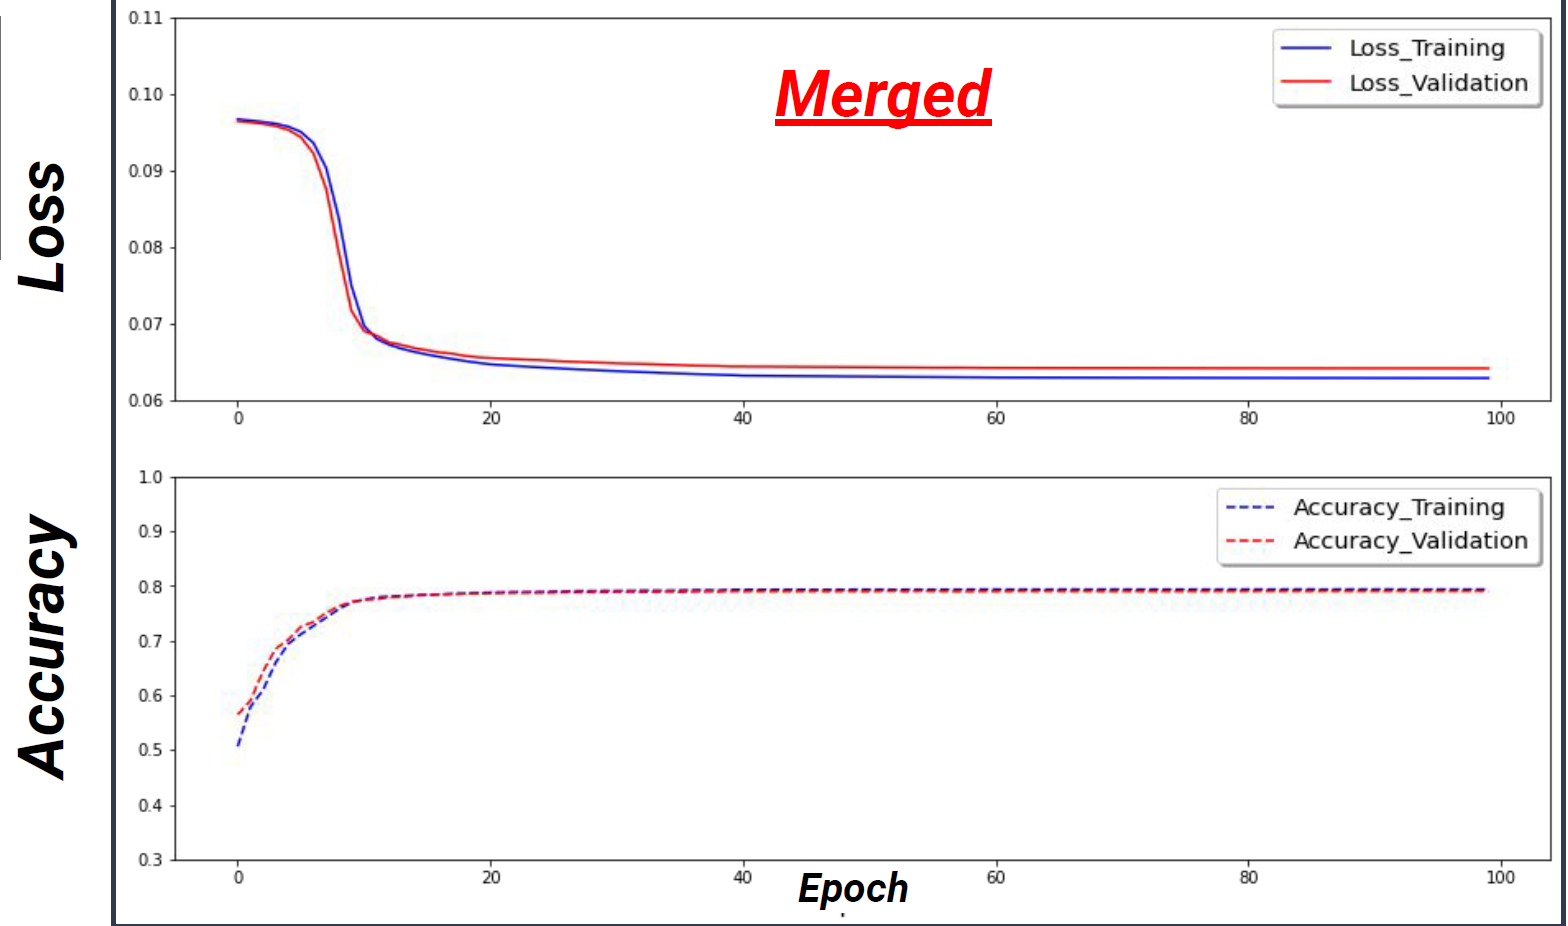
\includegraphics[width=0.45\textwidth]{figures/ml_dnn/loss_mer.png}}
       \subfloat[\emph{Loss curve}]{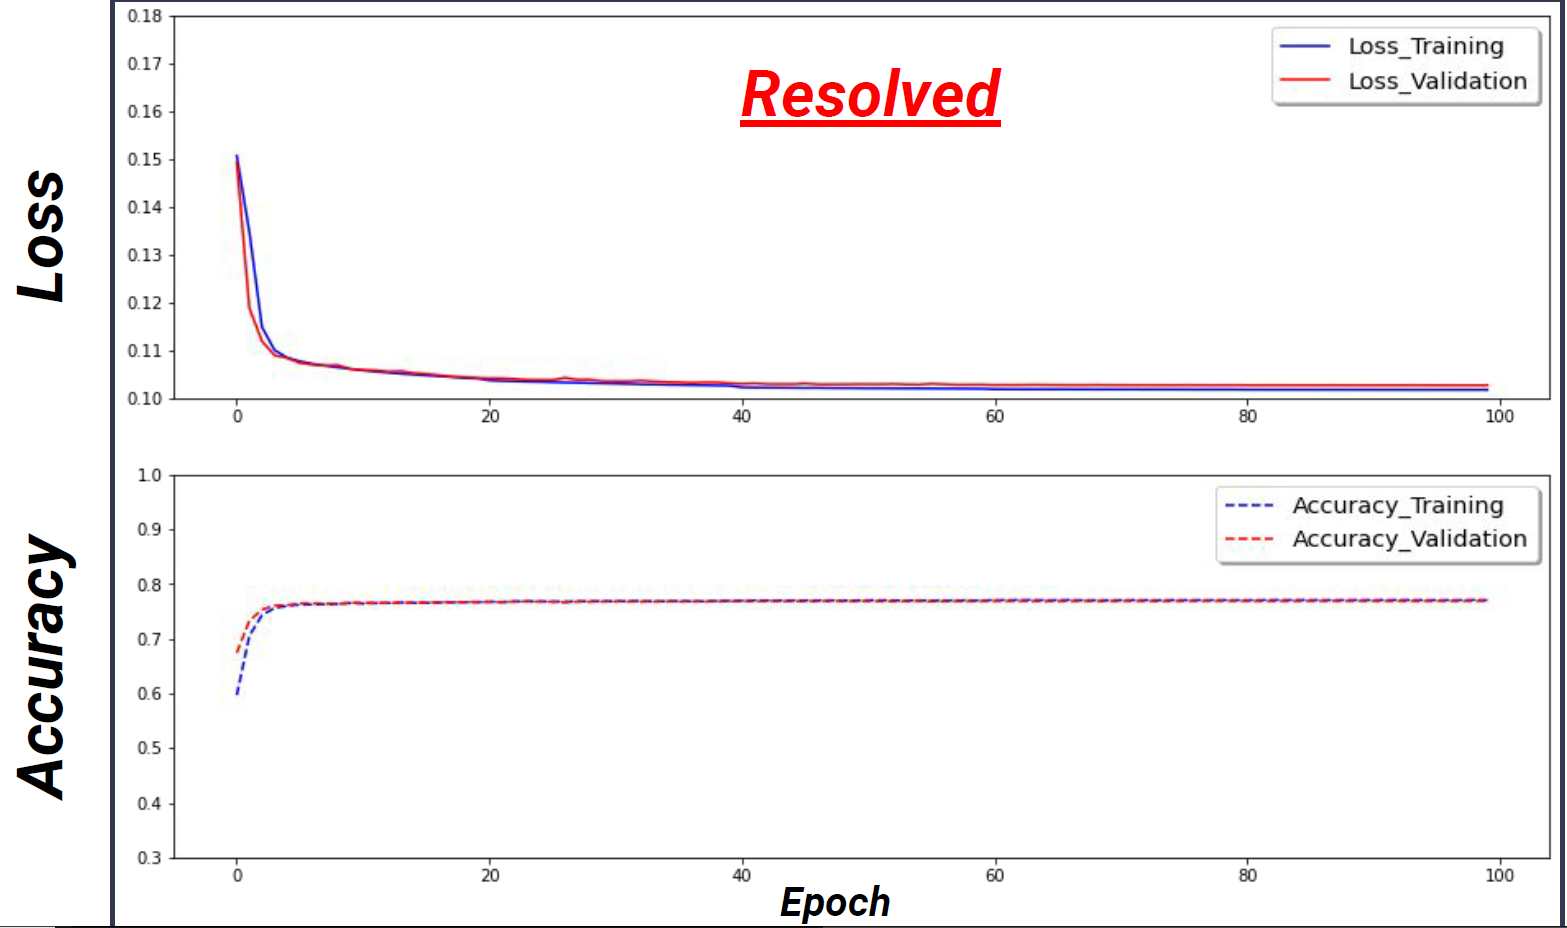
\includegraphics[width=0.45\textwidth]{figures/ml_dnn/loss_res.png}}
       \caption{Trainings for the DNN models in the merged and resolved regimes.}
       \label{fig:LossAndAccuracy}
\end{figure}

\begin{figure}[ht]
      \centering
       \subfloat[\emph{ROC curve}]{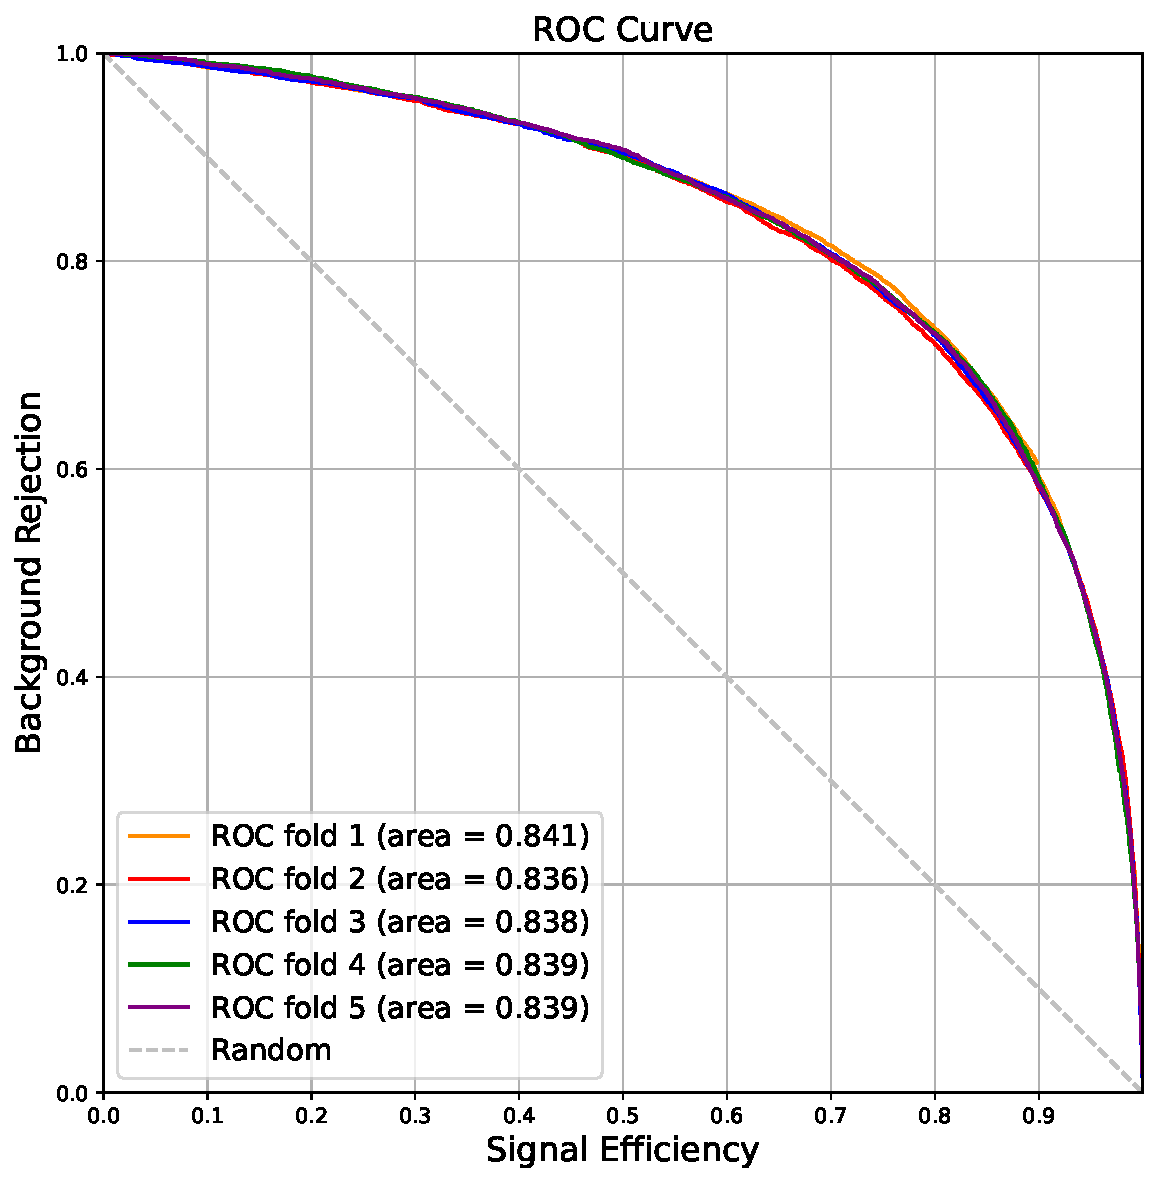
\includegraphics[width=0.45\textwidth]{figures/ml_dnn/kfold/roc_curve_mer.pdf}}
       \subfloat[\emph{ROC curve}]{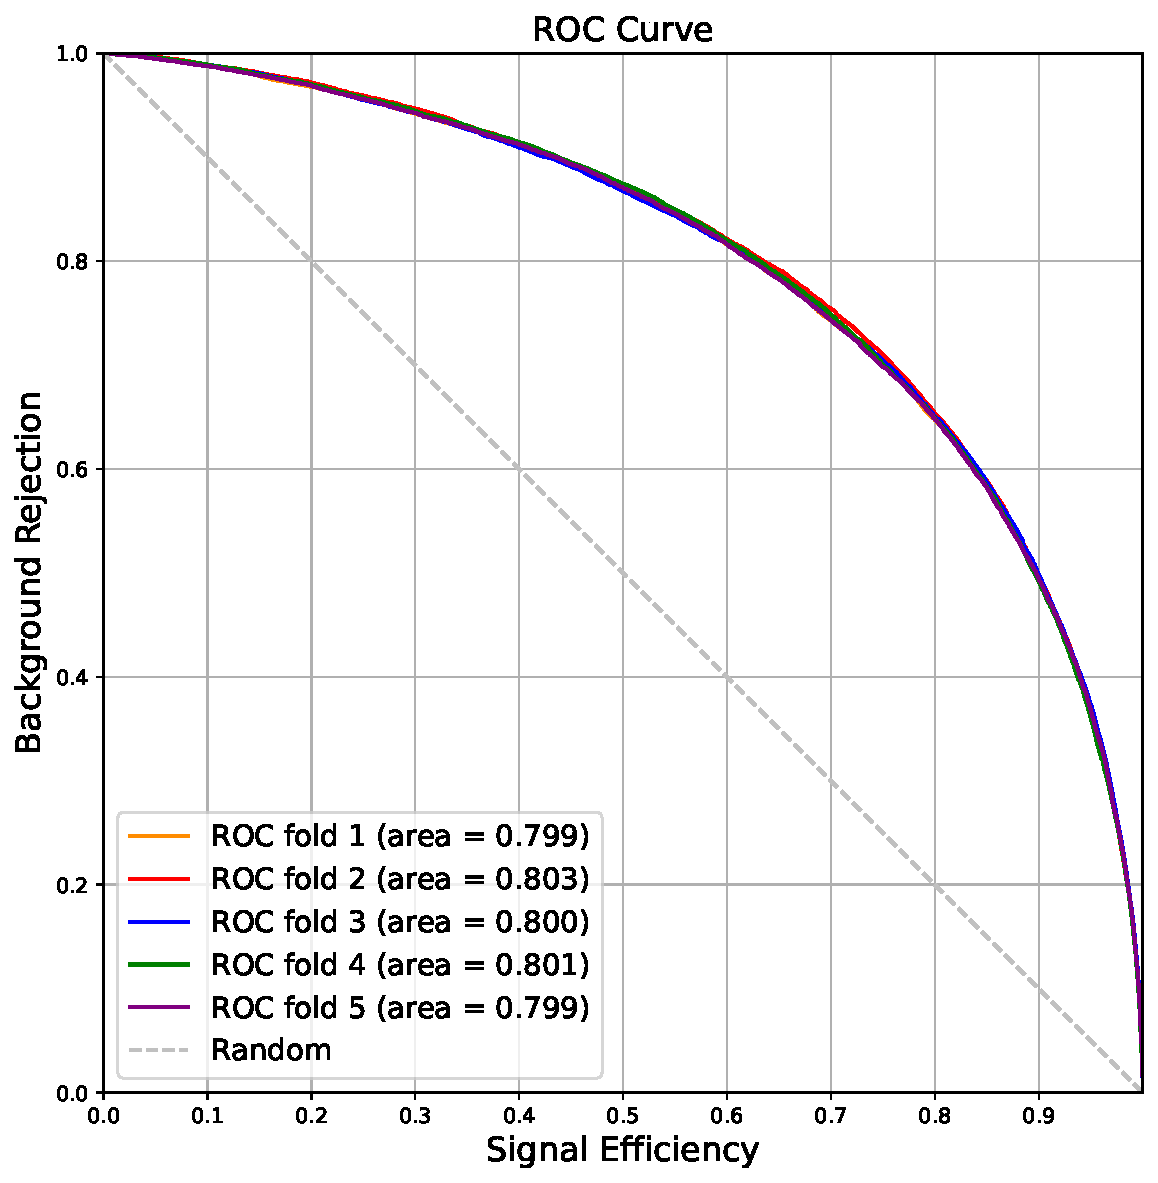
\includegraphics[width=0.45\textwidth]{figures/ml_dnn/kfold/roc_curve_res.pdf}}
       \caption{K-fold cross-validation for the DNN model trained in the merged and resolved regimes.}
       \label{fig:kfoldValidations}
\end{figure}


\begin{figure}[ht]
      \centering
       \subfloat[\emph{ROC curve}]{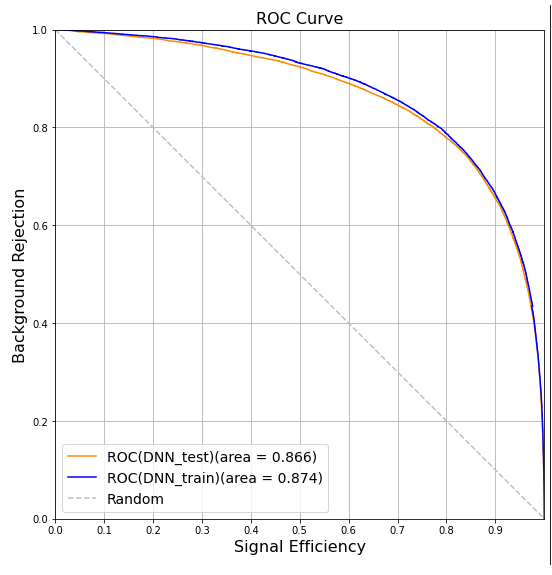
\includegraphics[width=0.45\textwidth]{figures/ml_dnn/roc_mer.png}}
       \subfloat[\emph{ROC curve}]{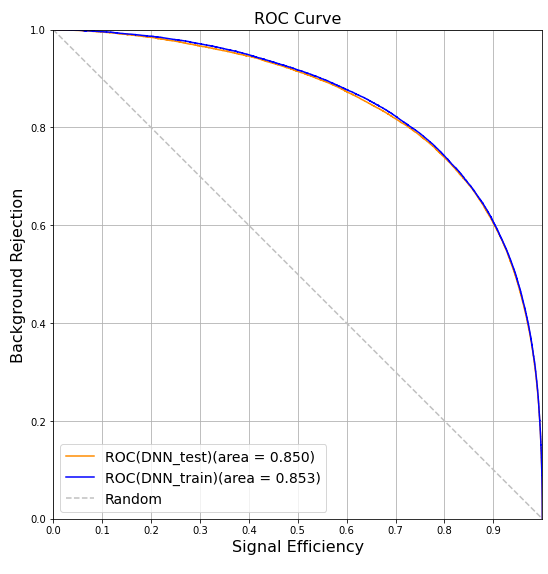
\includegraphics[width=0.45\textwidth]{figures/ml_dnn/roc_res.png}}
       \caption{Validation for the DNN model trained in the merged and resolved regimes.}
       \label{fig:ROCValidations}
\end{figure}

\begin{figure}[ht]
      \centering
       \subfloat[\emph{DNN Merged}]{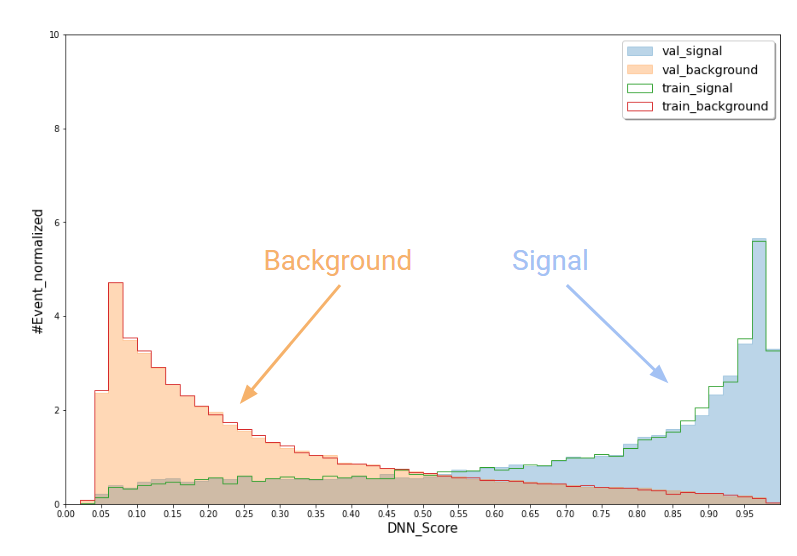
\includegraphics[width=0.45\textwidth]{figures/ml_dnn/dnn_dist/dnn_norm_mer.PNG}}
       \subfloat[\emph{DNN Resolved}]{\includegraphics[width=0.45\textwidth]{figures/ml_dnn/dnn_dist/dnn_norm_res.PNG}}
       \caption{Performance for the DNN model trained in the merged and resolved regimes.}
       \label{fig:1lepDNN_performance}
\end{figure}

\begin{figure}[ht]
 \begin{center}
  \subfloat[DNN HP]{\includegraphics[width=0.3\textwidth]{figures/ml_dnn/Region_distDNN_DSRVBSHP_BMin0_J0_incJet1_L1_T0_incFat1_Y6051_incTag1_Fat1_Prefit.pdf}}
  \subfloat[DNN LP]{\includegraphics[width=0.3\textwidth]{figures/ml_dnn/Region_distDNN_DSRVBSLP_BMin0_J0_incJet1_L1_T0_incFat1_Y6051_incTag1_Fat1_Prefit.pdf}}
  \subfloat[DNN Res]{\includegraphics[width=0.3\textwidth]{figures/ml_dnn/Region_distDNN_DSRVBSTight_BMin0_T0_Y6051_incTag1_J2_L1_incJet1_Prefit.pdf}}
  \caption{DNN score distributions for the high purity merged, low purity merged, and resolved signal regions.}
 \label{fig:1lepDNNoutputs}
 \end{center}
\end{figure}




\appendix
\chapter{An Appendix}\label{appendix:ATLAS_detector}

Appendix text goes here.


\backmatter

\bibliographystyle{bib/JHEP}
%\bibliographystyle{plain}
\bibliography{bib/refs,bib/ATLAS_papers}

\end{document}
\endinput
